\newpage
\section{实验}
\label{sec:experiment}

\subsection{数据准备}

\subsubsection{商品数据}

为了更好地开展商品信息相关的实验、测试,现以Product-10K数据集\cite{bai2020products10k}中的商品图片为基础,利用本地部署的多模态LLM批量生成这些商品对应的商品信息,再将这些信息输入到中心服务器中,以达到替代实际商品商品信息的目的。该数据集中的图片以存货单位(SKU)、商品类别为分类方式。在本实验中属于同一SKU的图片将被视为同一个商品的图片,每个SKU都会被随机挑出一个图片作为其代表交由LLM进行处理。文字部分利用的LLM是30亿参数版本 \verb|qwen2.5| 。

本实验利用本地部署的80亿参数版本 \verb|minicpm-v| 大模型进行商品图像描述的编写,使用的提示词对话如下:

\begin{itemize}
    \item[] \textbf{用户:}
    \begin{itemize}
        \item[] \textbf{(商品图片数据)}
        \item[] \textbf{(文字消息)} 细致地描述这个图片中的内容,以便其他模型利用这段描述进行进一步推理。
    \end{itemize}
\end{itemize}

然而,对生成结果(及其对应图片)的人工抽查显示数据集中某些图片更加接近生活照片,难以被断定为商品图片。因此,以下的提示词对话被用于检测图片是否代表一个商品:

\begin{itemize}
    \item[] \textbf{用户:} 以下是从一个图片产生的说明,请根据这段说明判断该图片是否表示一个商品(布尔值字段verdict):\textit{(商品图片描述)}
\end{itemize}

以上提示词在使用的时候加入了对模型输出的限制(具有布尔值字段 \verb|verdict| 的JSON对象)。经过筛选之后的商品图片描述其后进入商品描述生成的过程:

\begin{itemize}
    \item[] \textbf{用户:} 请编写商品描述,商品描述应该尽可能有吸引力,并且不要输出商品描述之外的内容。以下是商品对应图片的描述:\textit{(商品图片描述)}
\end{itemize}

最后,生成的商品描述被用于进一步生成商品标题:

\begin{itemize}
    \item[] \textbf{用户:} 为这段商品介绍产生一个言简意赅的商品标题:\textit{(商品描述)}
\end{itemize}

生成的商品标题、描述等数据其后被收集起来,并且与其图片相绑定。之后,这些数据被通过第 \ref{sec:foundation} 部分提及的服务器API传输到数据库中,用于后续试验。

\subsubsection{销售数据}

考虑到本设计的高度实验性,试图在实际销售场景上运用该项目对应的程序实现是并不现实的。为了在这种情况下继续有关销售数据分析的实验,在此采用Kaggle内容发布者yapwh1208的“Supermarket Sales Data”数据集\footnote{数据集主页:https://www.kaggle.com/datasets/yapwh1208/supermarket-sales-data}(按发布者声明内容采集自“全国大学生数学建模竞赛\footnote{官方网站:https://www.mcm.edu.cn/}”相关数据集)。该数据包含在三年间的采集自(生鲜)超市的每笔交易的质量、价格等相关信息。

\subsection{服务端}

\subsubsection{RmInit}

\begin{figure}[htbp]
    \subfloat{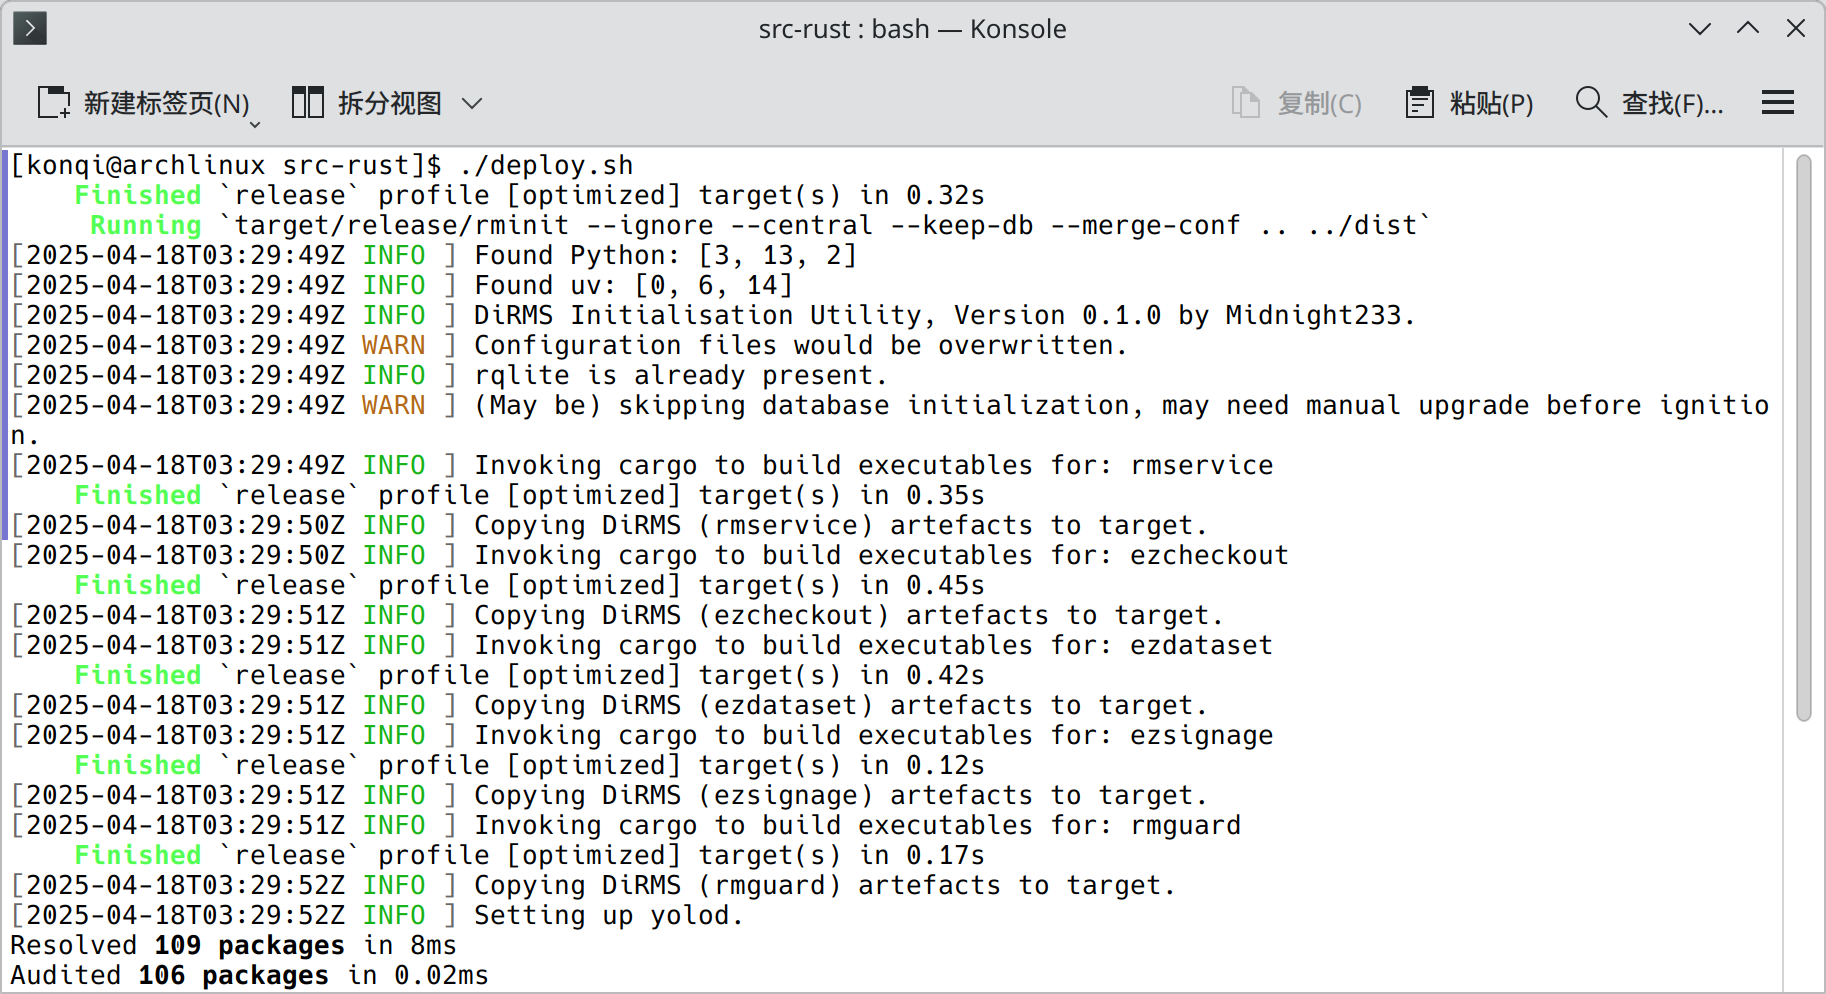
\includegraphics[width=0.45\textwidth]{./exp/rminit-1.png}}
    \hfill
    \subfloat{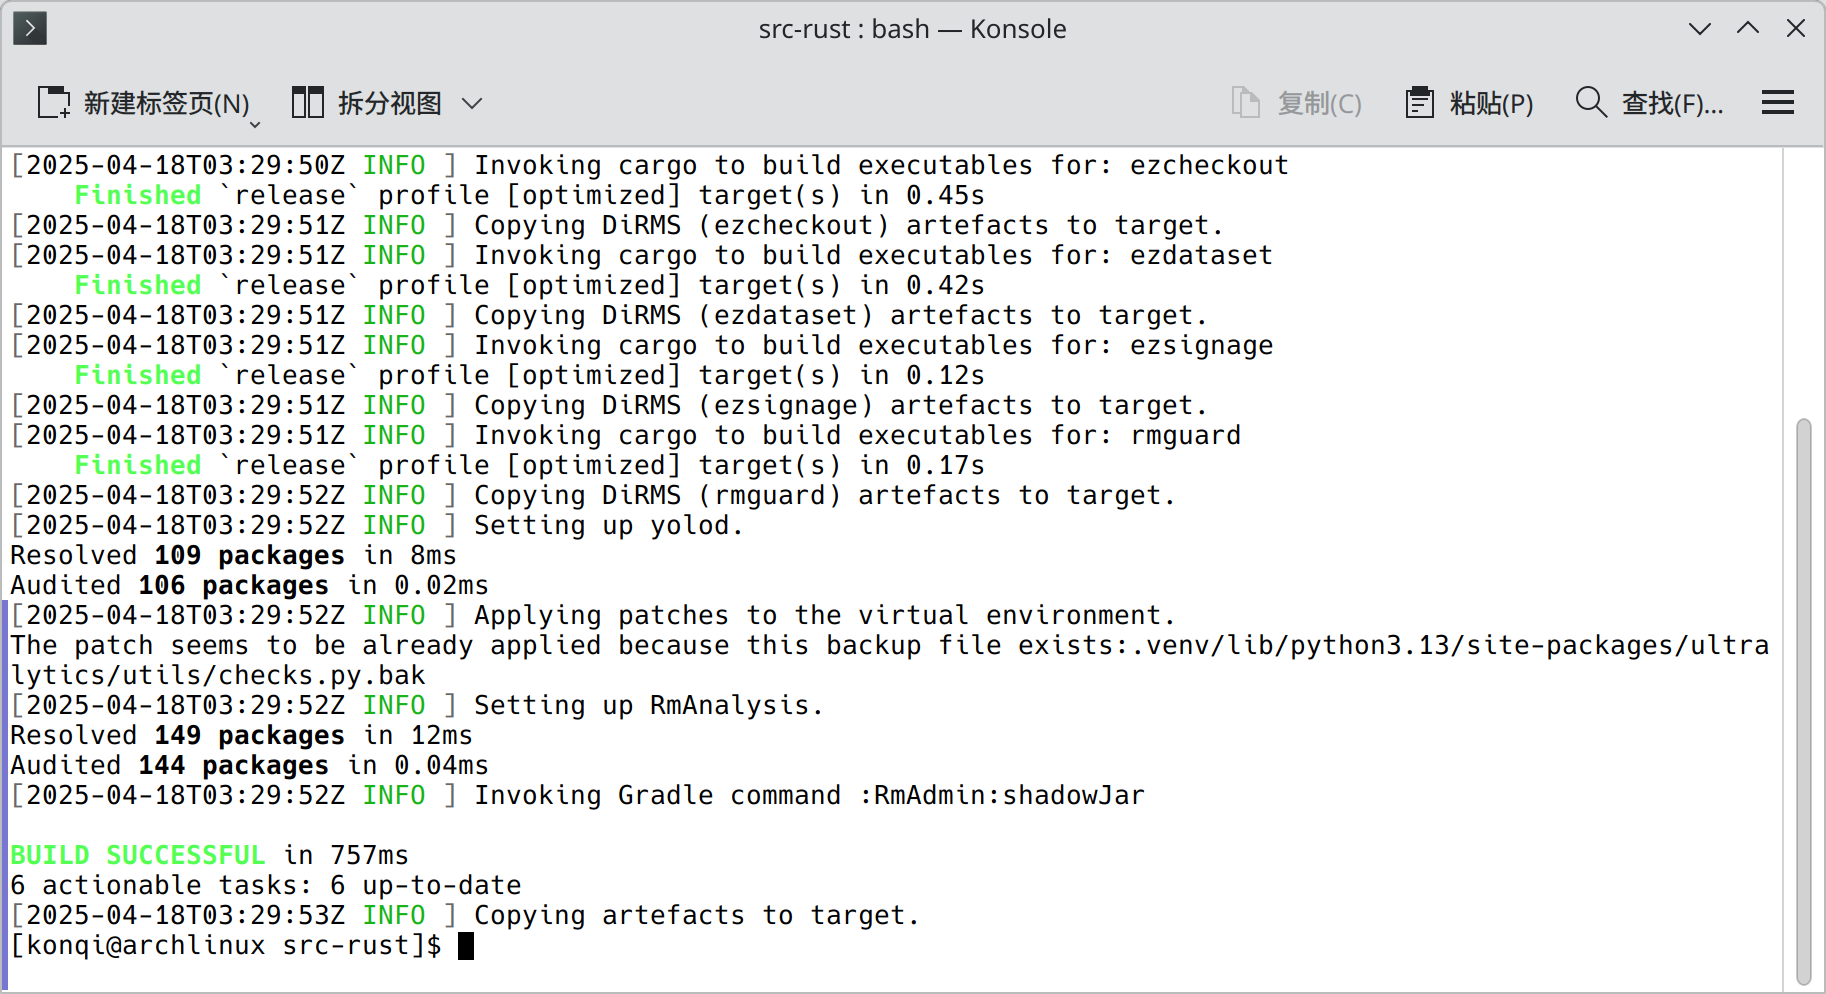
\includegraphics[width=0.45\textwidth]{./exp/rminit-2.png}}
	\caption{RmInit运行效果}
	\label{fig:rminit}
\end{figure}

 RmInit应用程序是面向零售系统整合商、技术能力较强的零售行业从业者的,用于自动编译、部署该设计的源代码发行版到指定文件夹。通过指定命令行开关,用户可以调整部署的方式和升级部署的时候覆盖的内容。本实验其余部分的应用程序来源于利用以下命令进行的部署:

\begin{verbatim}
cargo run --release --package rminit -- --ignore --central --keep-db \
--merge-conf .. ../dist
\end{verbatim}

\subsubsection{RmGuard}

\begin{figure}[htbp]
	\centering
	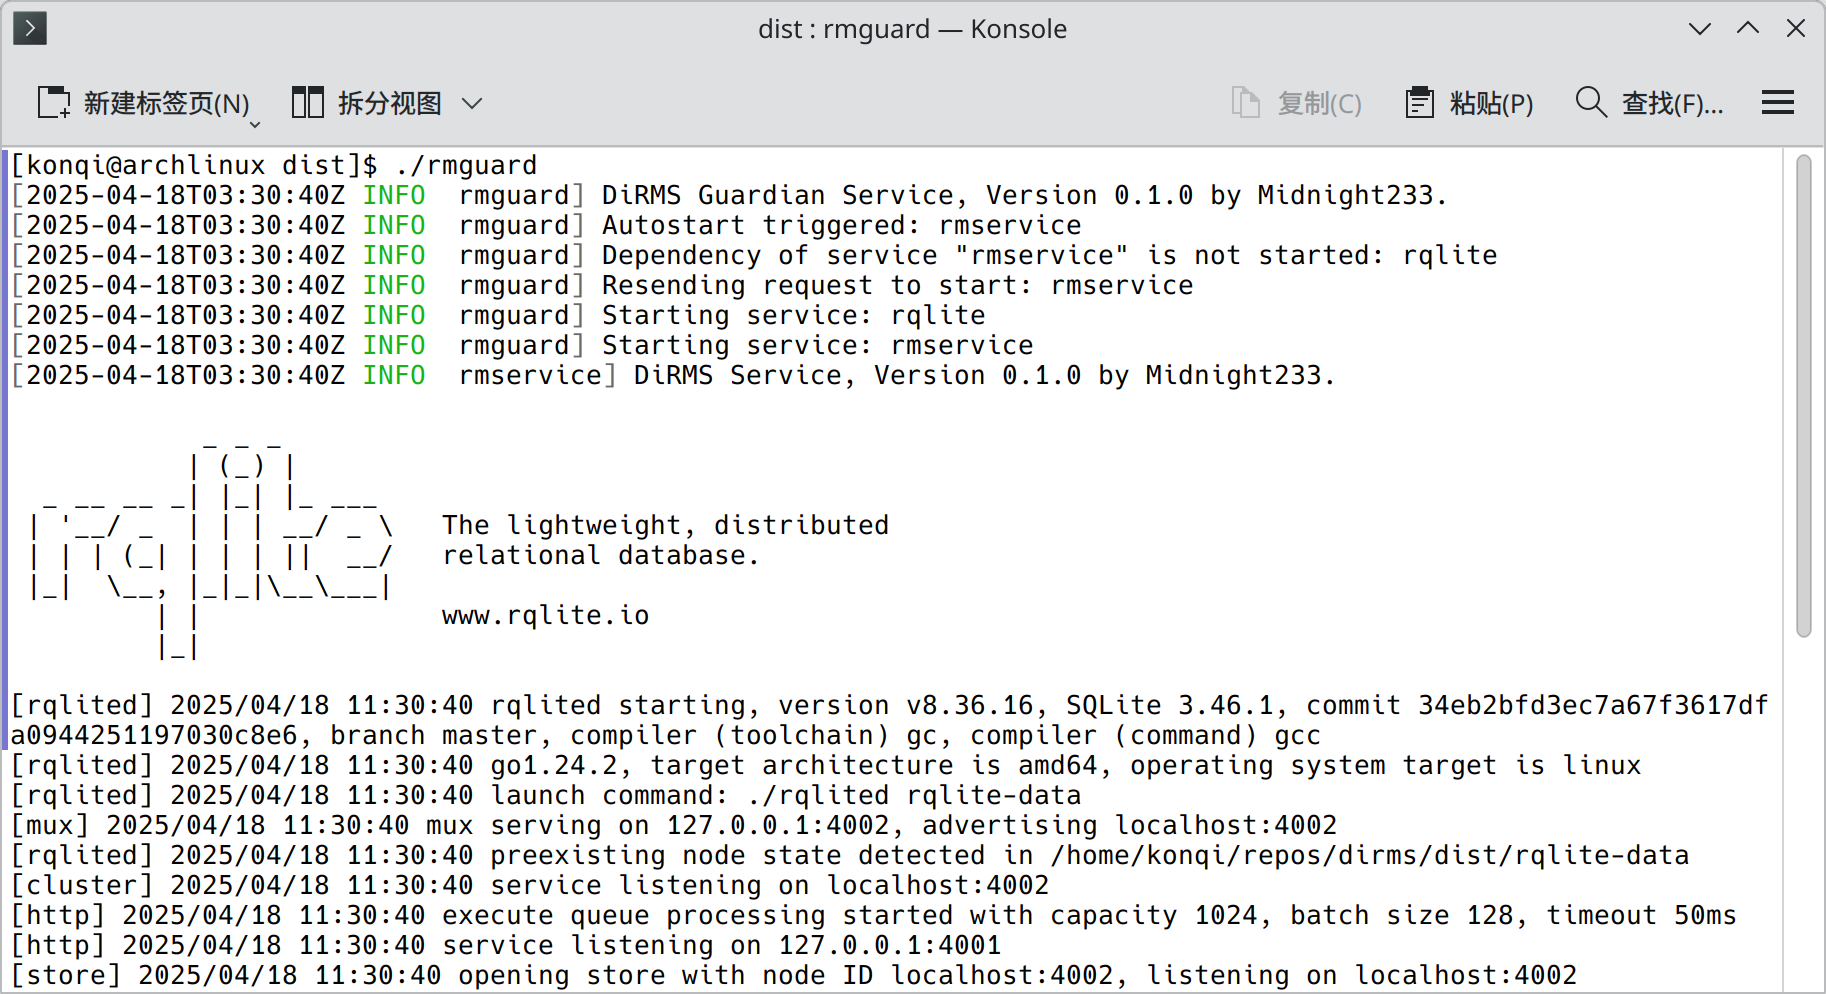
\includegraphics[width=0.8\textwidth]{./exp/rmg-core.png}
	\caption{RmGuard运行效果:启动核心服务}
	\label{fig:rmg-core}
\end{figure}

\begin{figure}[htbp]
    \subfloat{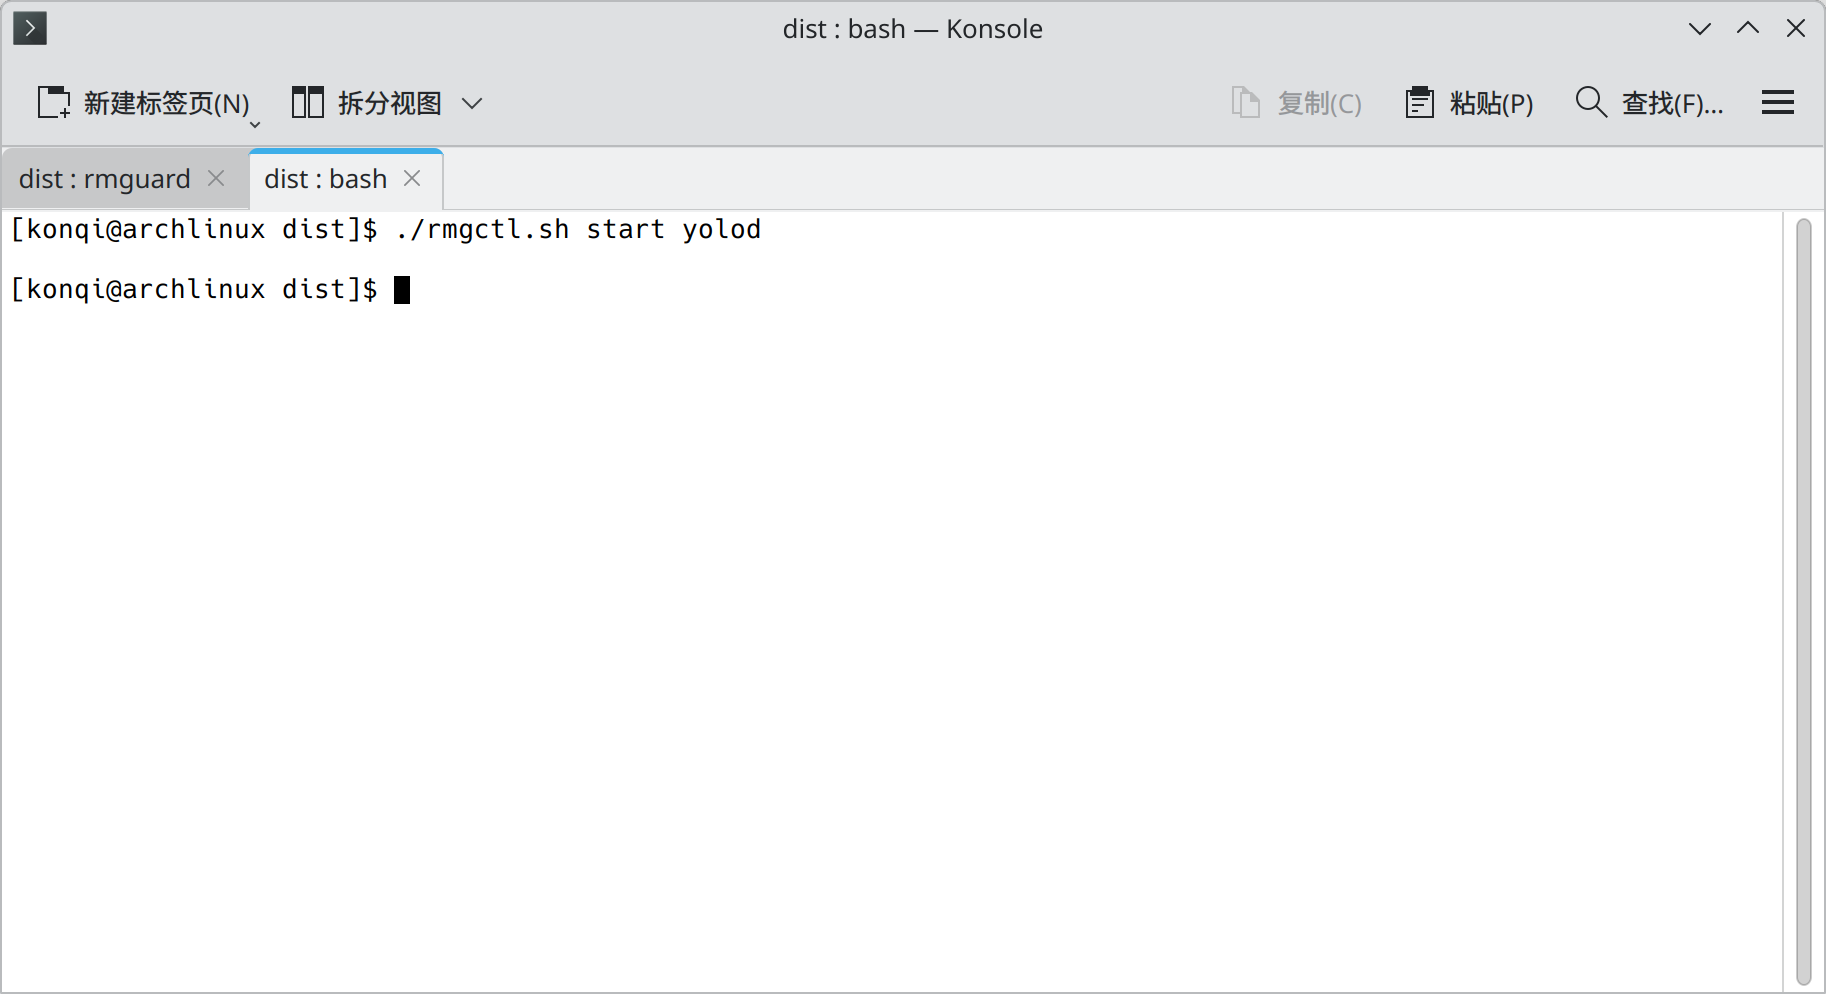
\includegraphics[width=0.45\textwidth]{./exp/rmg-yolod-1.png}}
    \hfill
    \subfloat{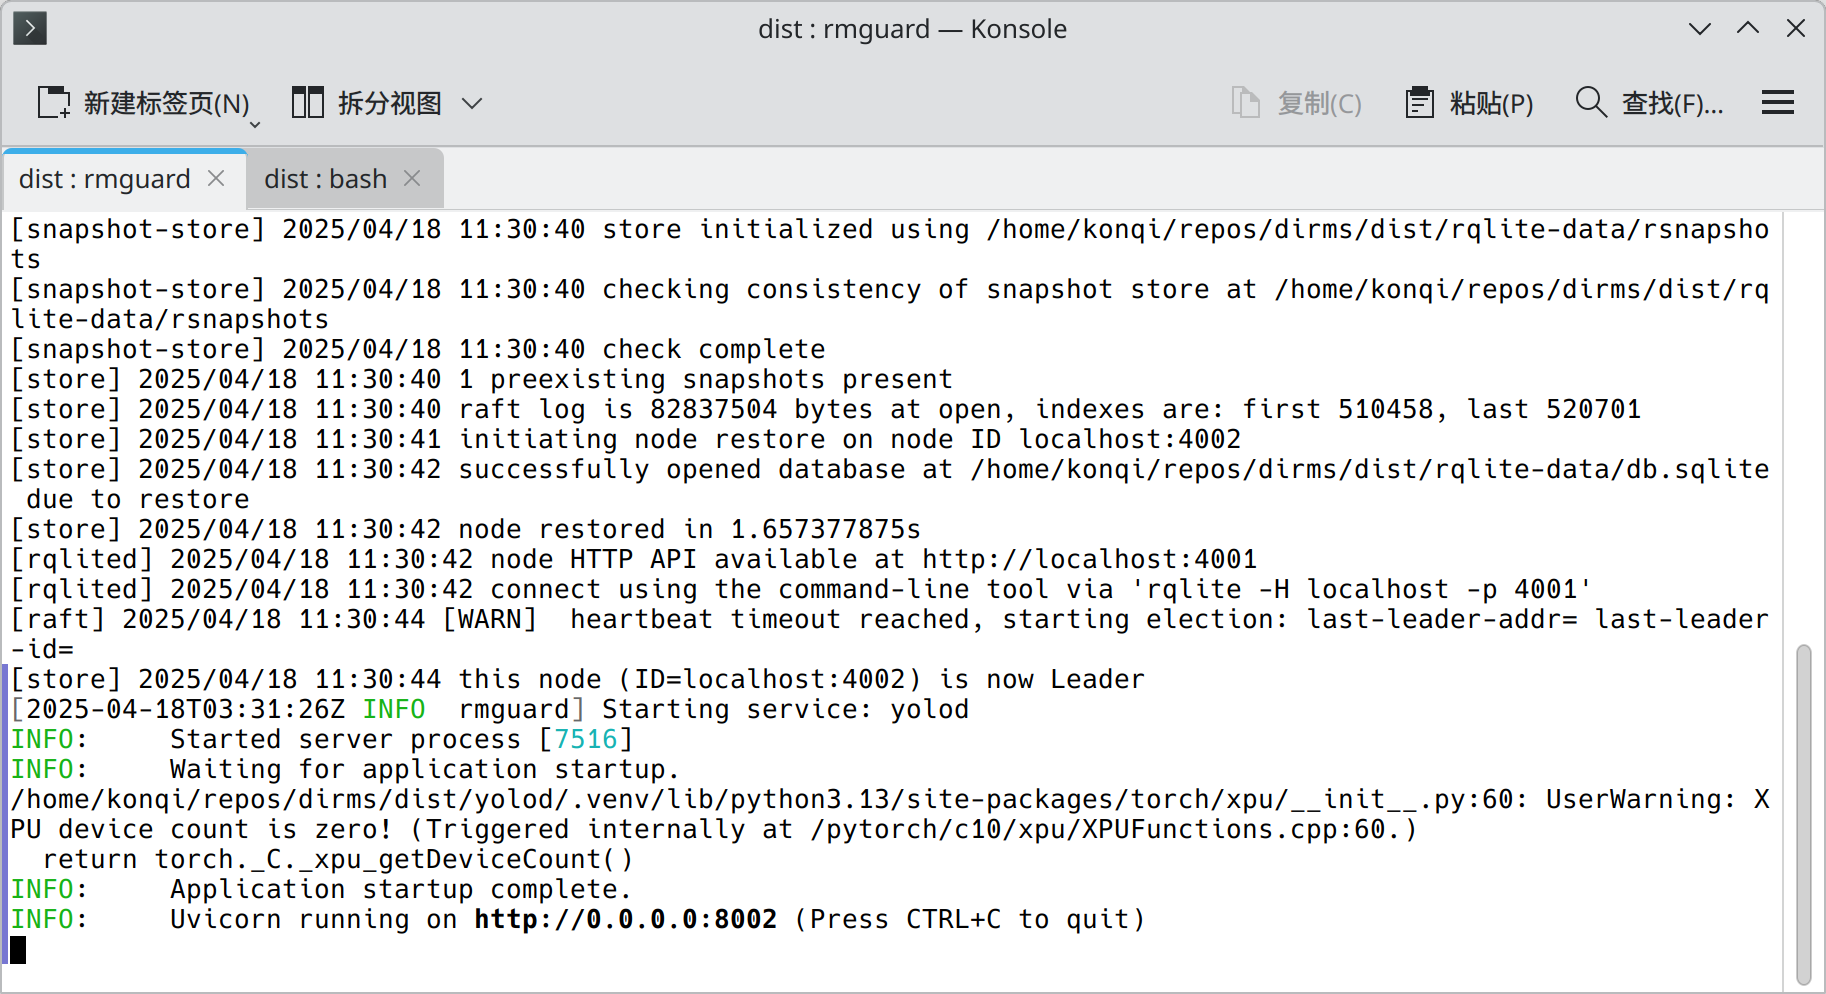
\includegraphics[width=0.45\textwidth]{./exp/rmg-yolod-2.png}}
    \vspace{1em}
    \subfloat{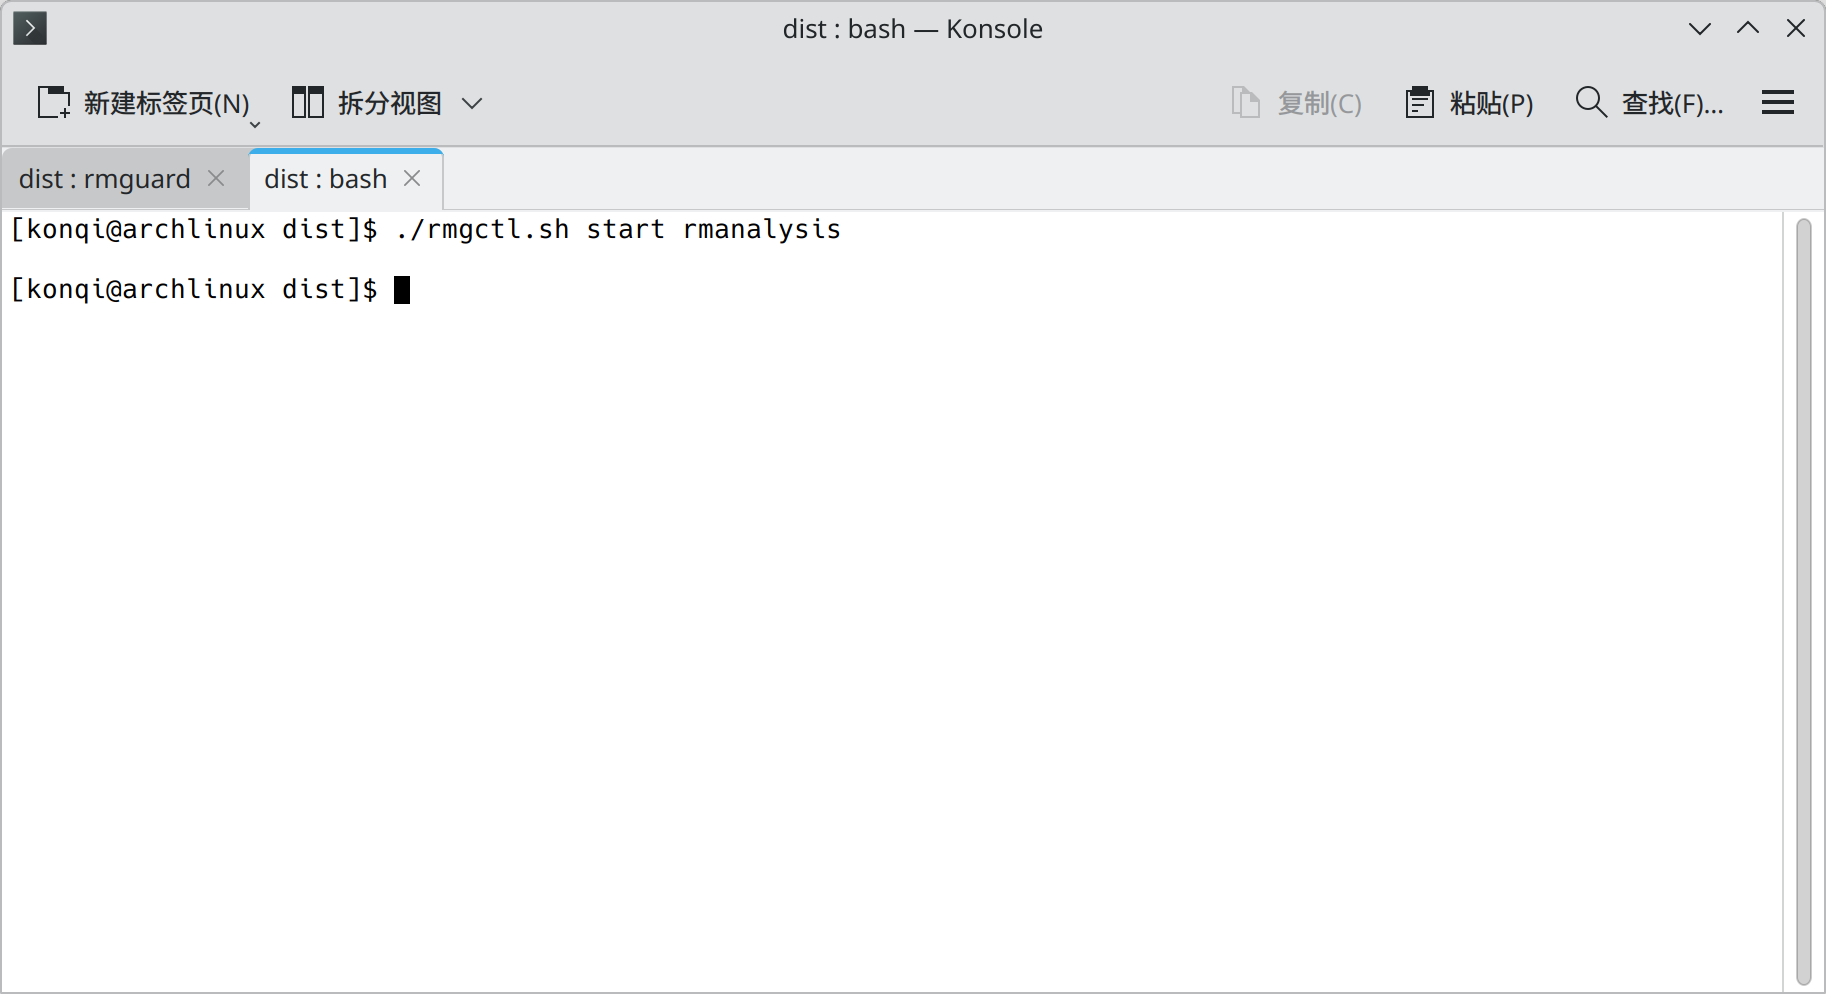
\includegraphics[width=0.45\textwidth]{./exp/rmg-rma-1.png}}
    \hfill
    \subfloat{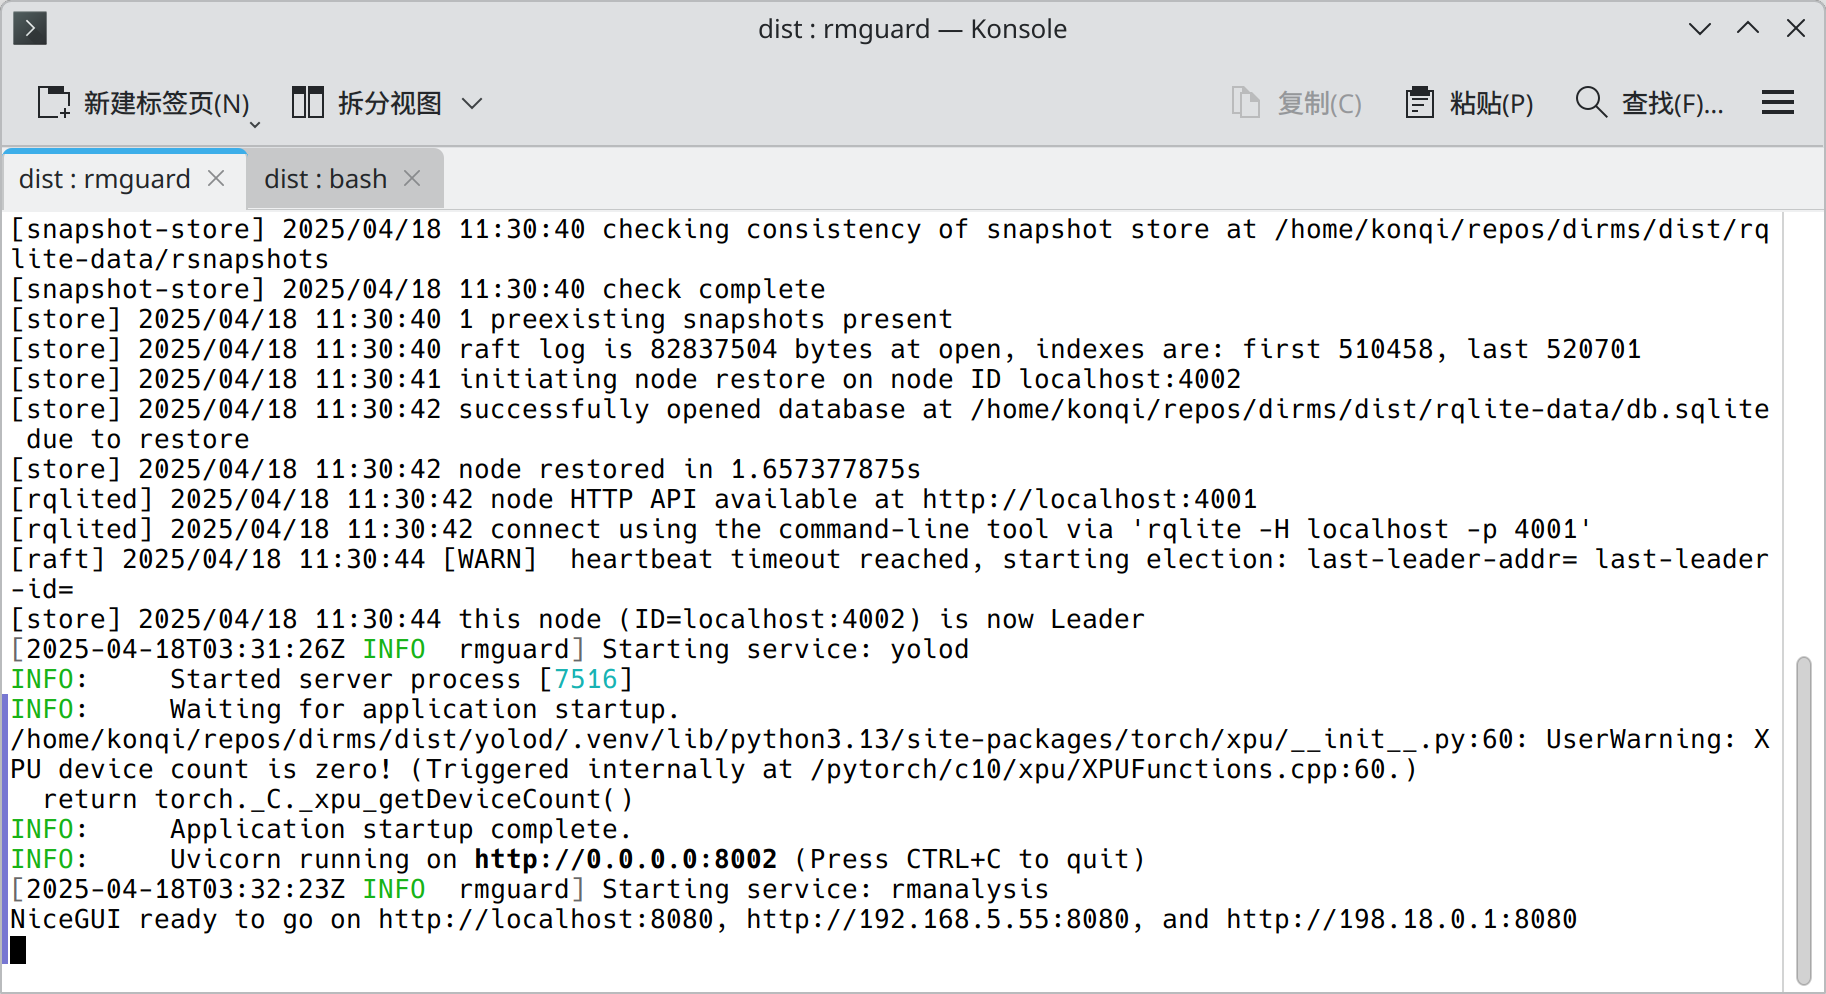
\includegraphics[width=0.45\textwidth]{./exp/rmg-rma-2.png}}
	\caption{RmGuard运行效果:启动核心服务}
	\label{fig:rmg-service}
\end{figure}

RmGuard是用于设计中不同的服务子系统之间运行时依赖关系的、自启动管理的应用程序。如图 \ref{fig:rmg-core} 所示,通过在配置文件之中编写如下服务自启动要求,RmService及其依赖的rqlite服务将被按正确顺序启动:

\begin{verbatim}
[guard]
autostart = ["rmservice"]
\end{verbatim}

此外,通过脚本 \verb|rmgctl.sh|(RmGuard Controller)可以对所有服务进行状态查询和操控,如图 \ref{fig:rmg-service} 所示,尚未通过自动启动配置启动的 \verb|rmanalysis| 和 \verb|yolod| 服务可以使用这种方式进行启动。

\subsection{商家端}

\subsubsection{RmAdmin}

\begin{figure}[htbp]
	\centering
	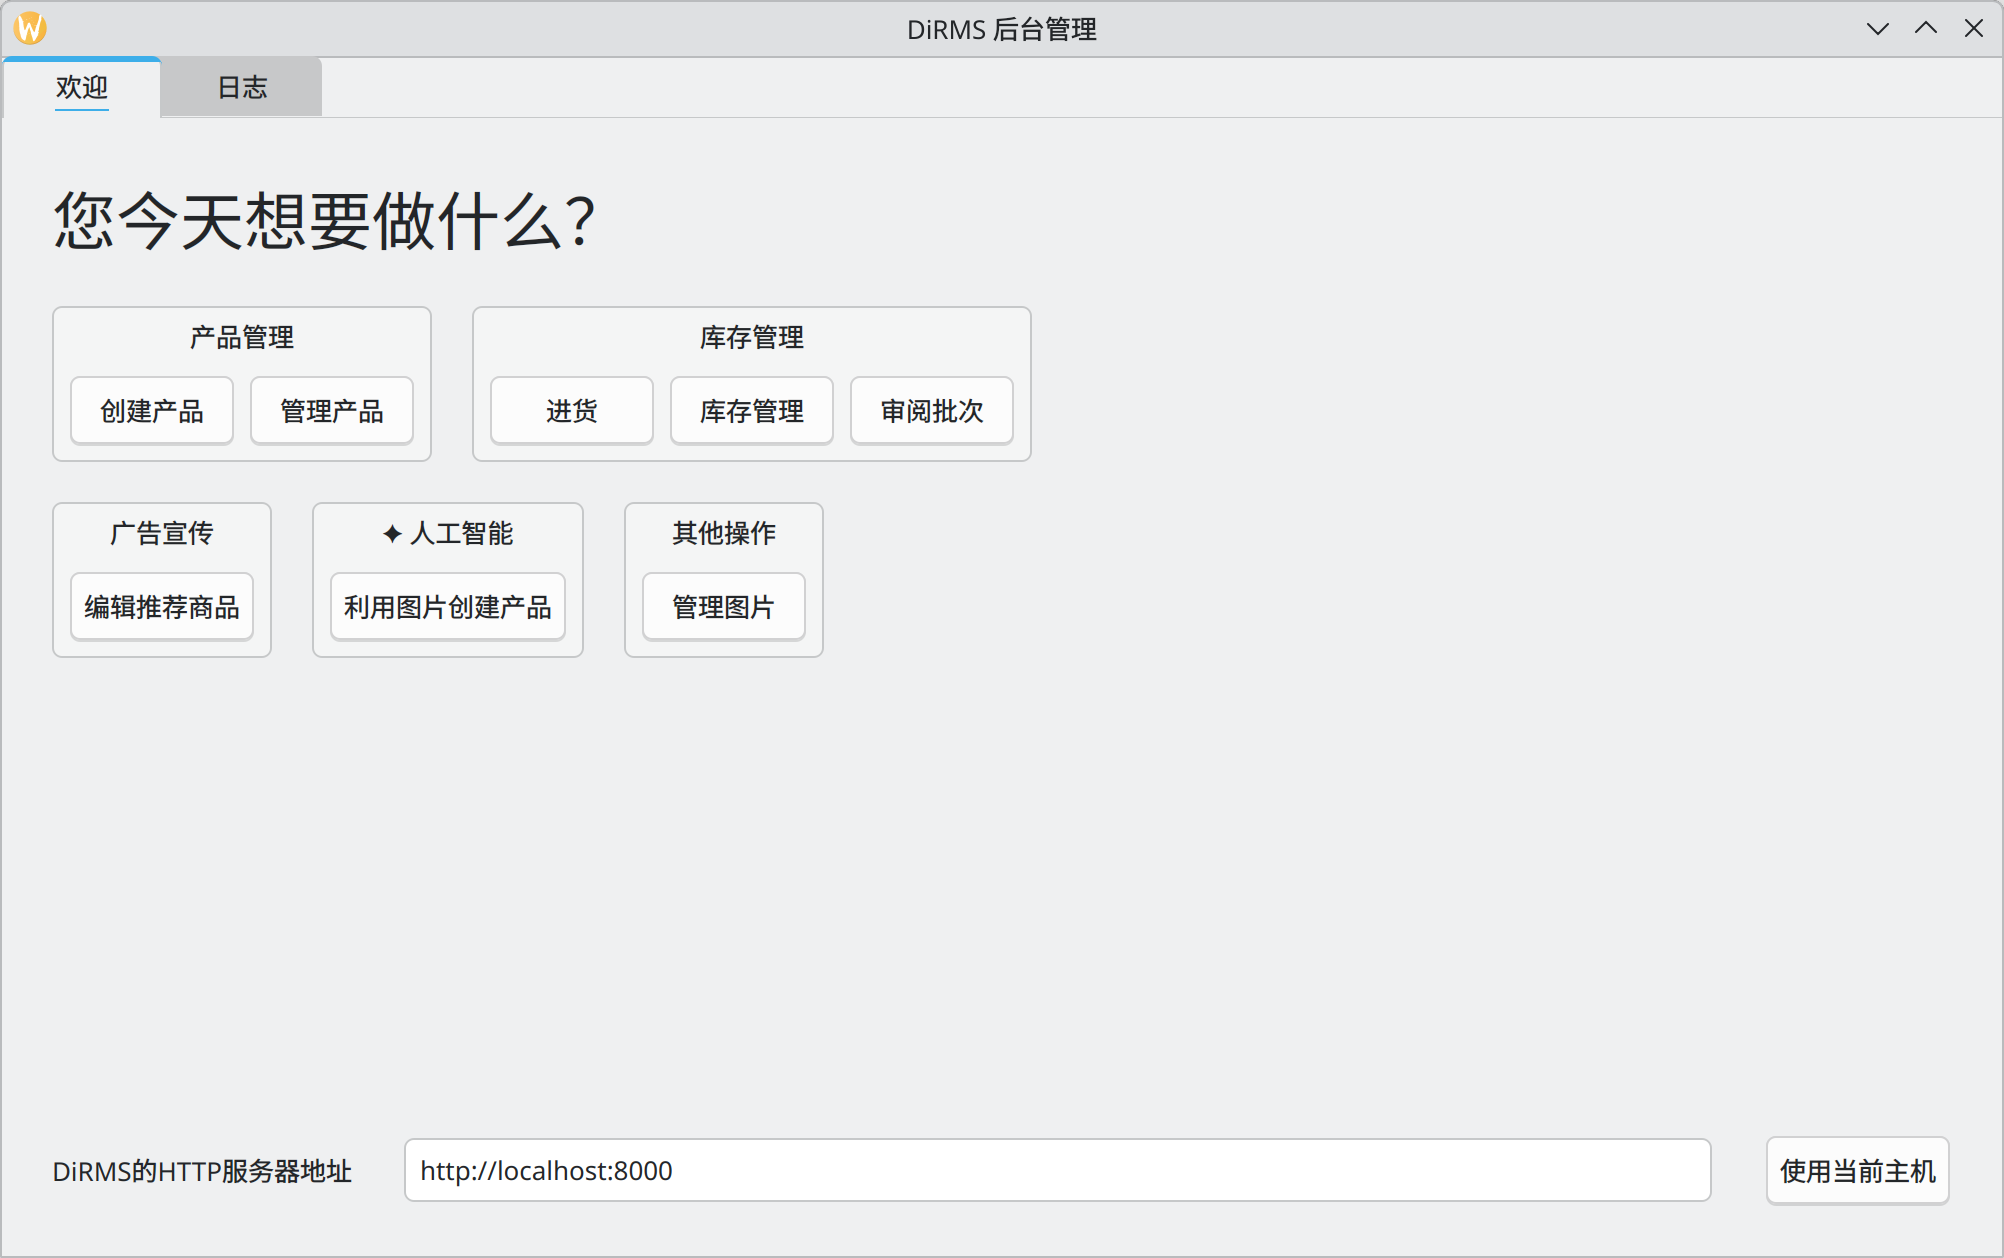
\includegraphics[width=0.8\textwidth]{./exp/rma-index.png}
	\caption{RmAdmin运行效果:首页}
	\label{fig:rma-index}
\end{figure}

RmAdmin是该设计所对应的商家端(即“后台管理”)应用程序,通过在如图 \ref{fig:rma-index} 所示的主界面选择所需的功能,用户可以对系统的不同部分(产品、库存、广告等)进行管理。同时,用户可以通过在画面底部的单行输入框中输入HTTP地址来指定进行操作的目标服务器。

\begin{figure}[htbp]
    \subfloat{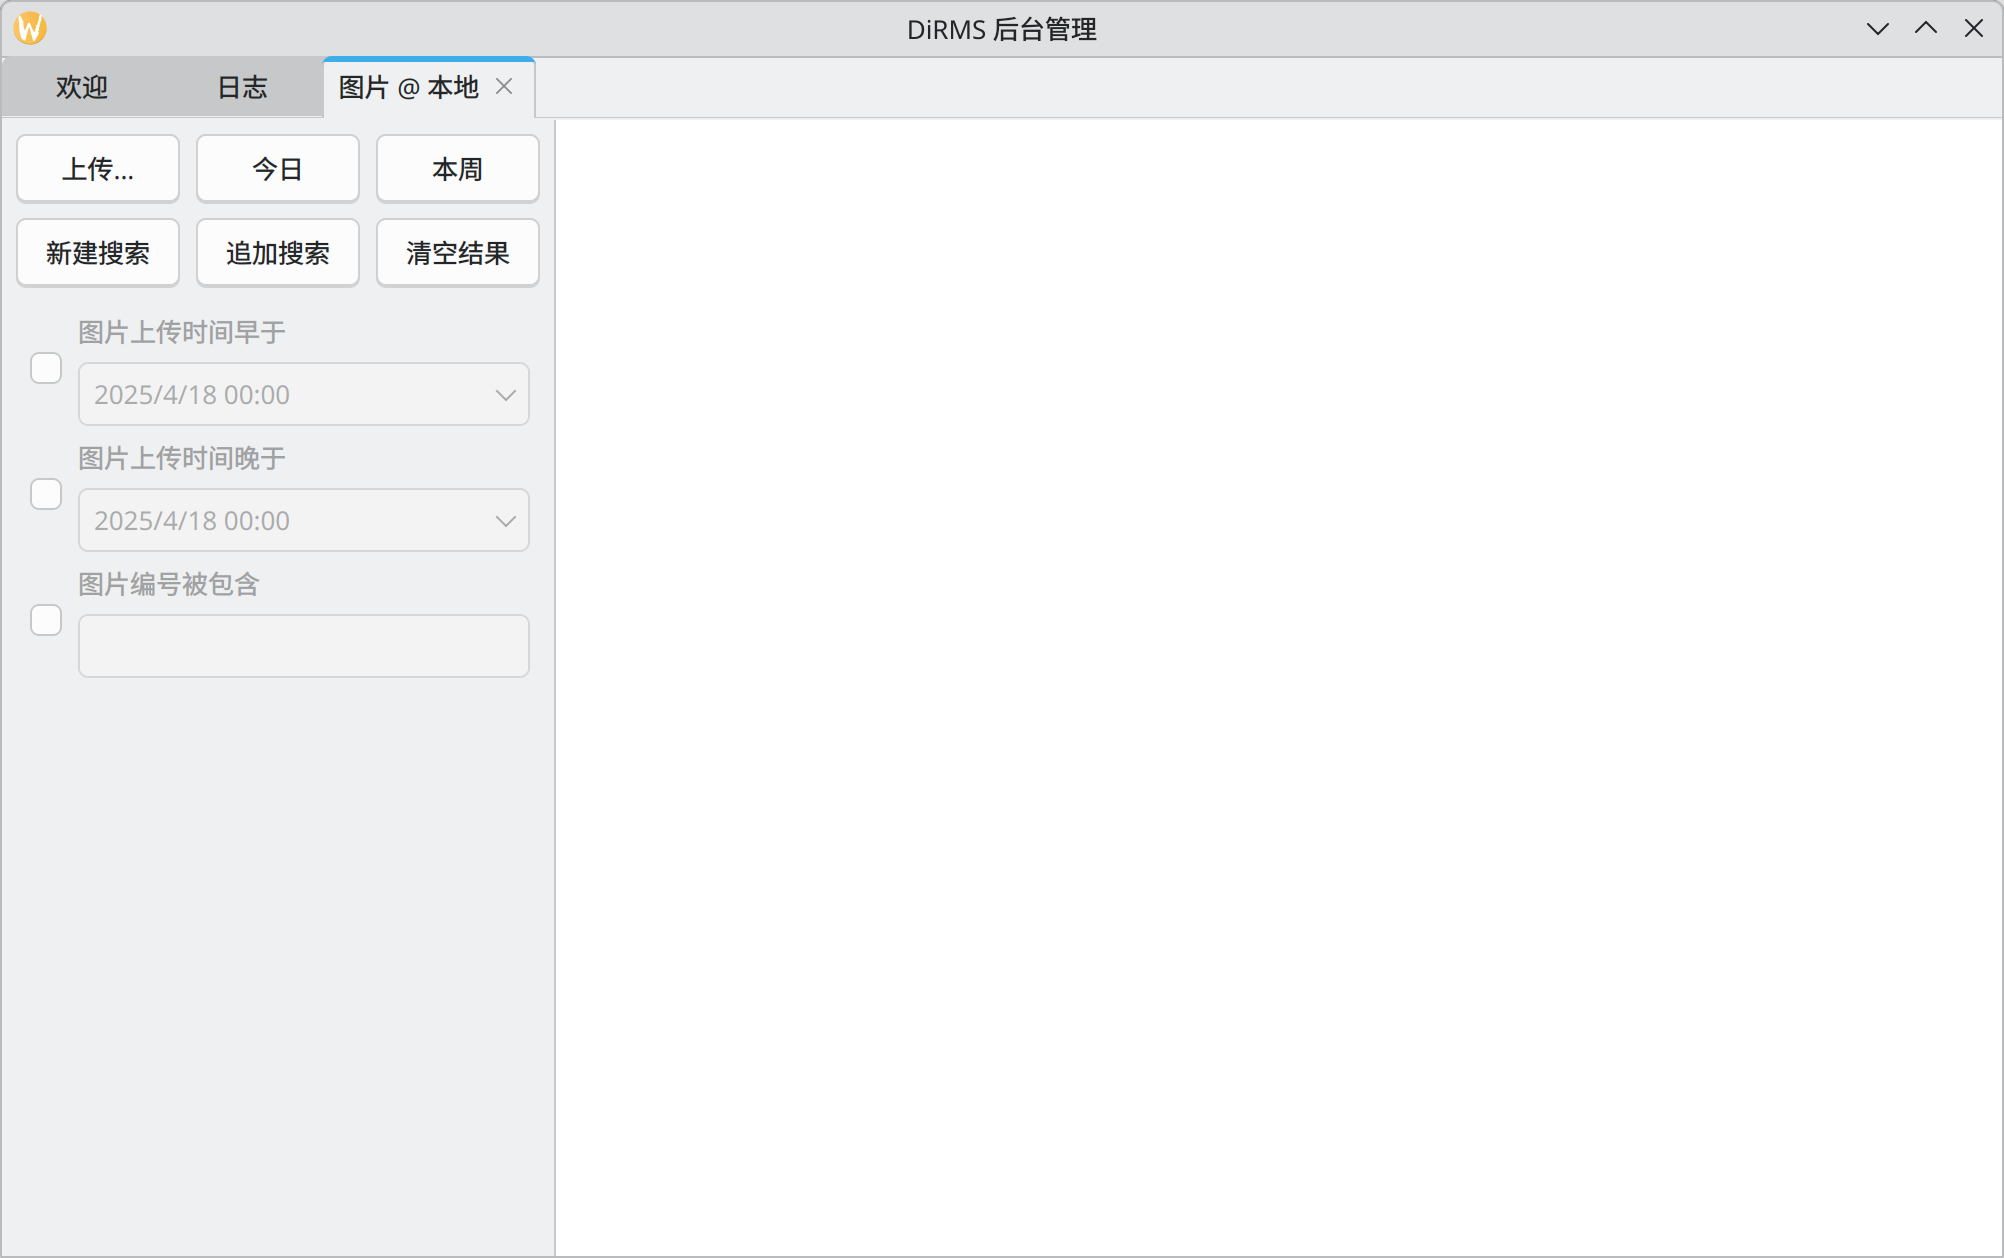
\includegraphics[width=0.45\textwidth]{./exp/rma-im-add-1.png}}
    \hfill
    \subfloat{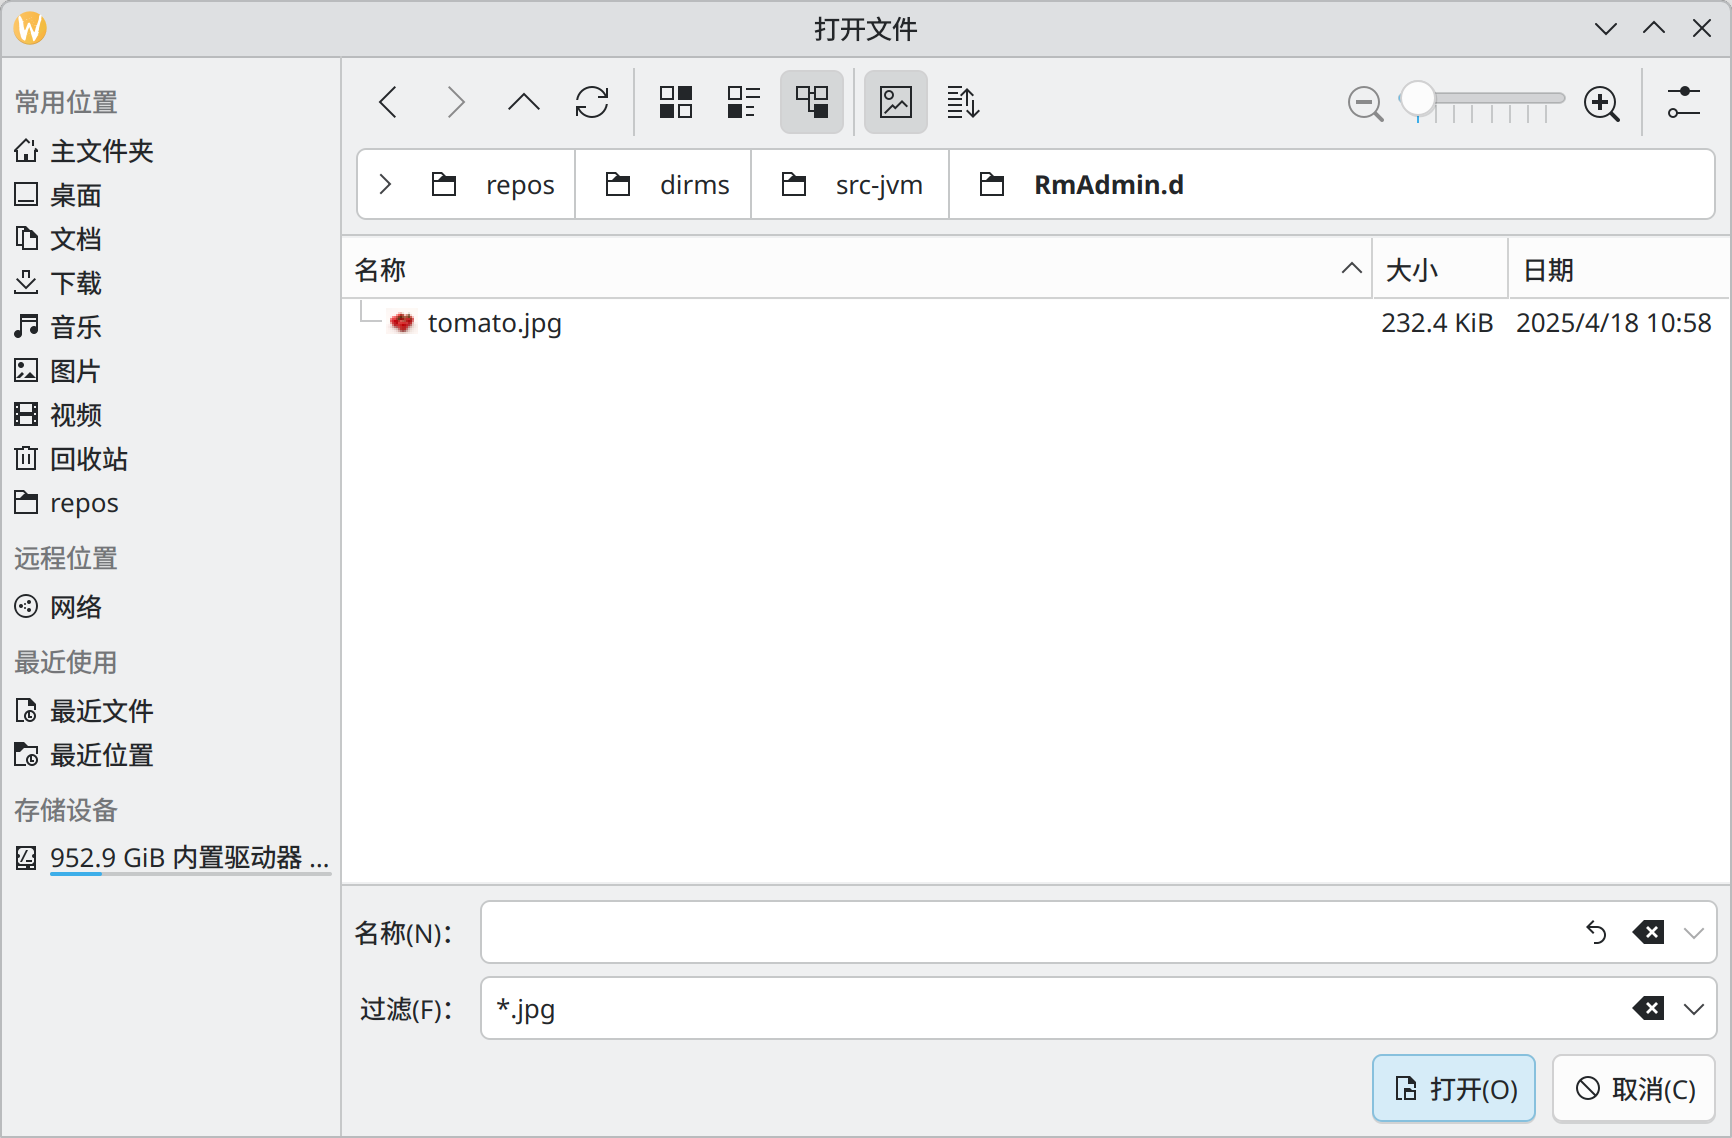
\includegraphics[width=0.45\textwidth]{./exp/rma-im-add-2.png}}
	\caption{RmAdmin运行效果:添加图片}
	\label{fig:rma-im-add}
\end{figure}

\begin{figure}[htbp]
	\centering
	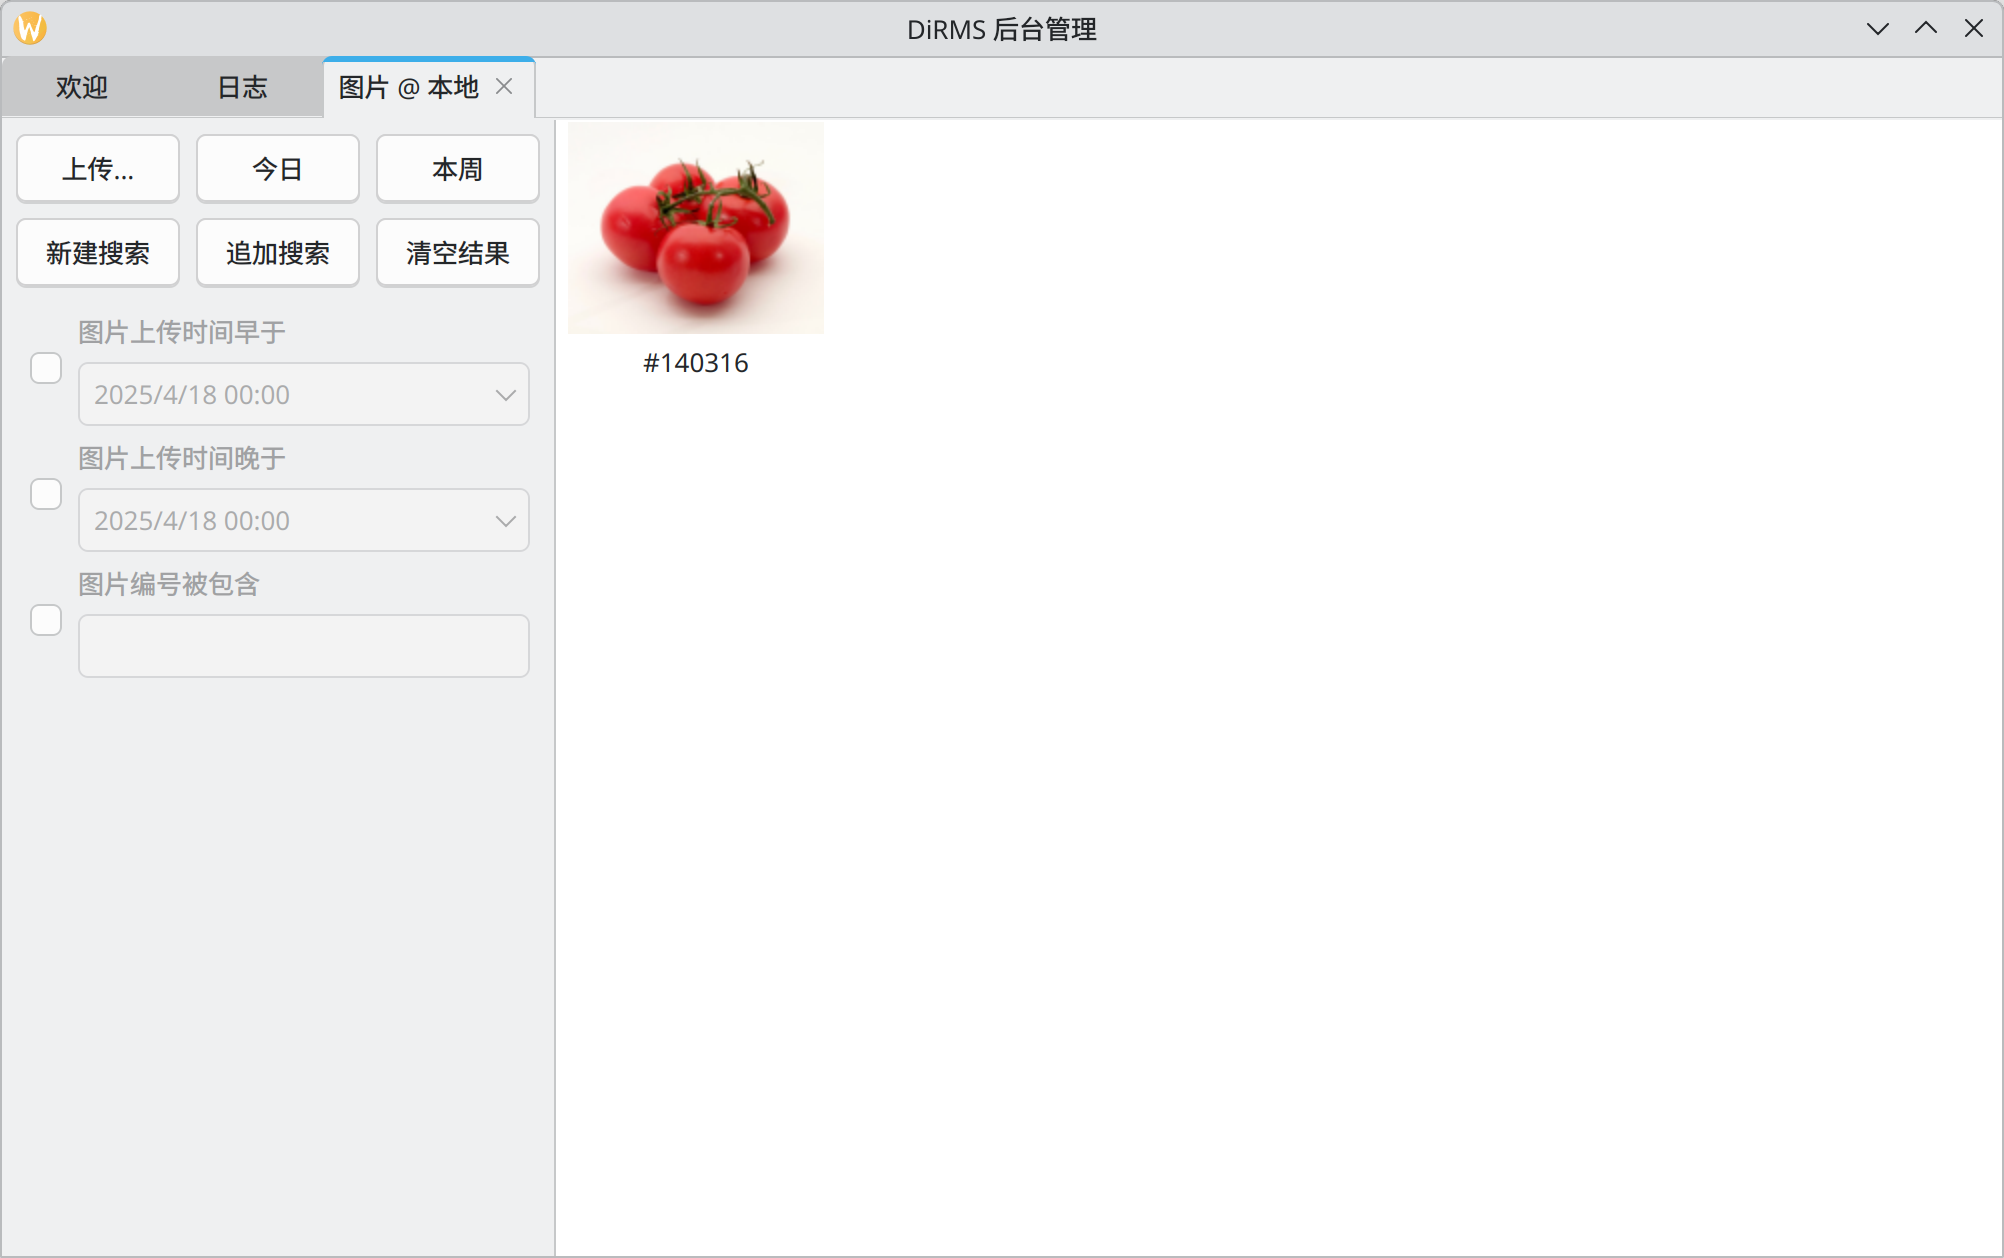
\includegraphics[width=0.8\textwidth]{./exp/rma-im-as.png}
	\caption{RmAdmin运行效果:图片高级搜索}
	\label{fig:rma-im-as}
\end{figure}

用于图片管理的界面如图 \ref{fig:rma-im-add} 左侧所示,用户可以在左上侧选择需要执行的操作,包括图像的上传、检索等。通过点击“上传\dots”按钮,用户可以在如图 \ref{fig:rma-im-add} 右侧所示(平台相关)的界面上进行图片的选择和提交。提交的图片会被通过HTTP API传输到服务器中,完成上传的过程。

界面正左侧部分(及部分左上侧按钮)为图片高级搜索功能。用户可以通过点击条件左侧复选框进行条件的启用或停用,并在条件名称以下的输入框中指定具体值,以此达到条件细致的搜索。常见的搜索条件(如“今日”和“本周”)则作为按钮给出,用户通过点击这些按钮可以轻松在海量商品图片中进行搜索。如图 \ref{fig:rma-im-as} 所示为点击“今日”产生的搜索结果(图片来自上文上传)。

\begin{figure}[htbp]
    \subfloat{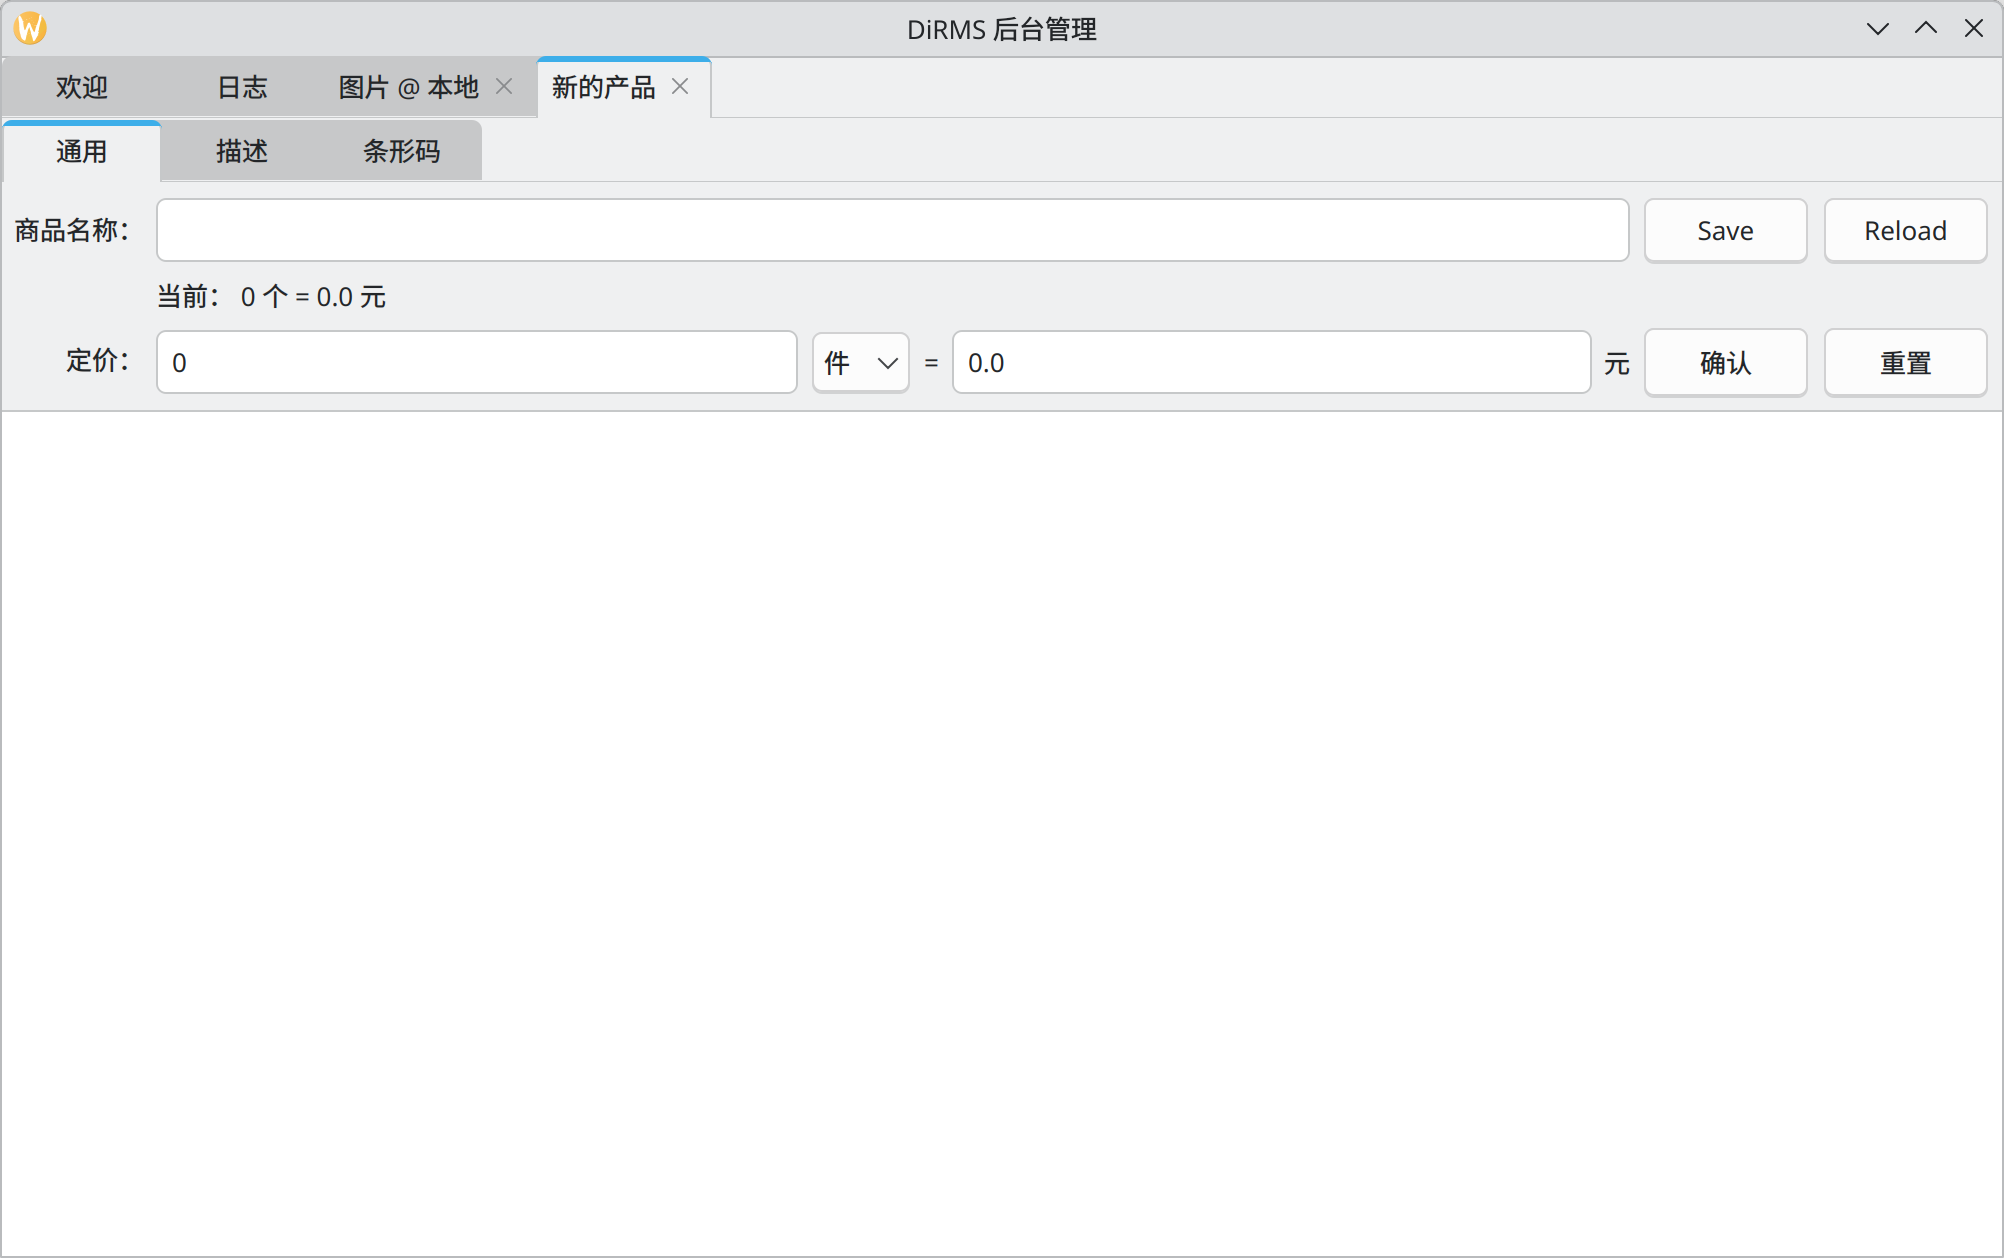
\includegraphics[width=0.3\textwidth]{./exp/rma-prod-add-1.png}}
    \hfill
    \subfloat{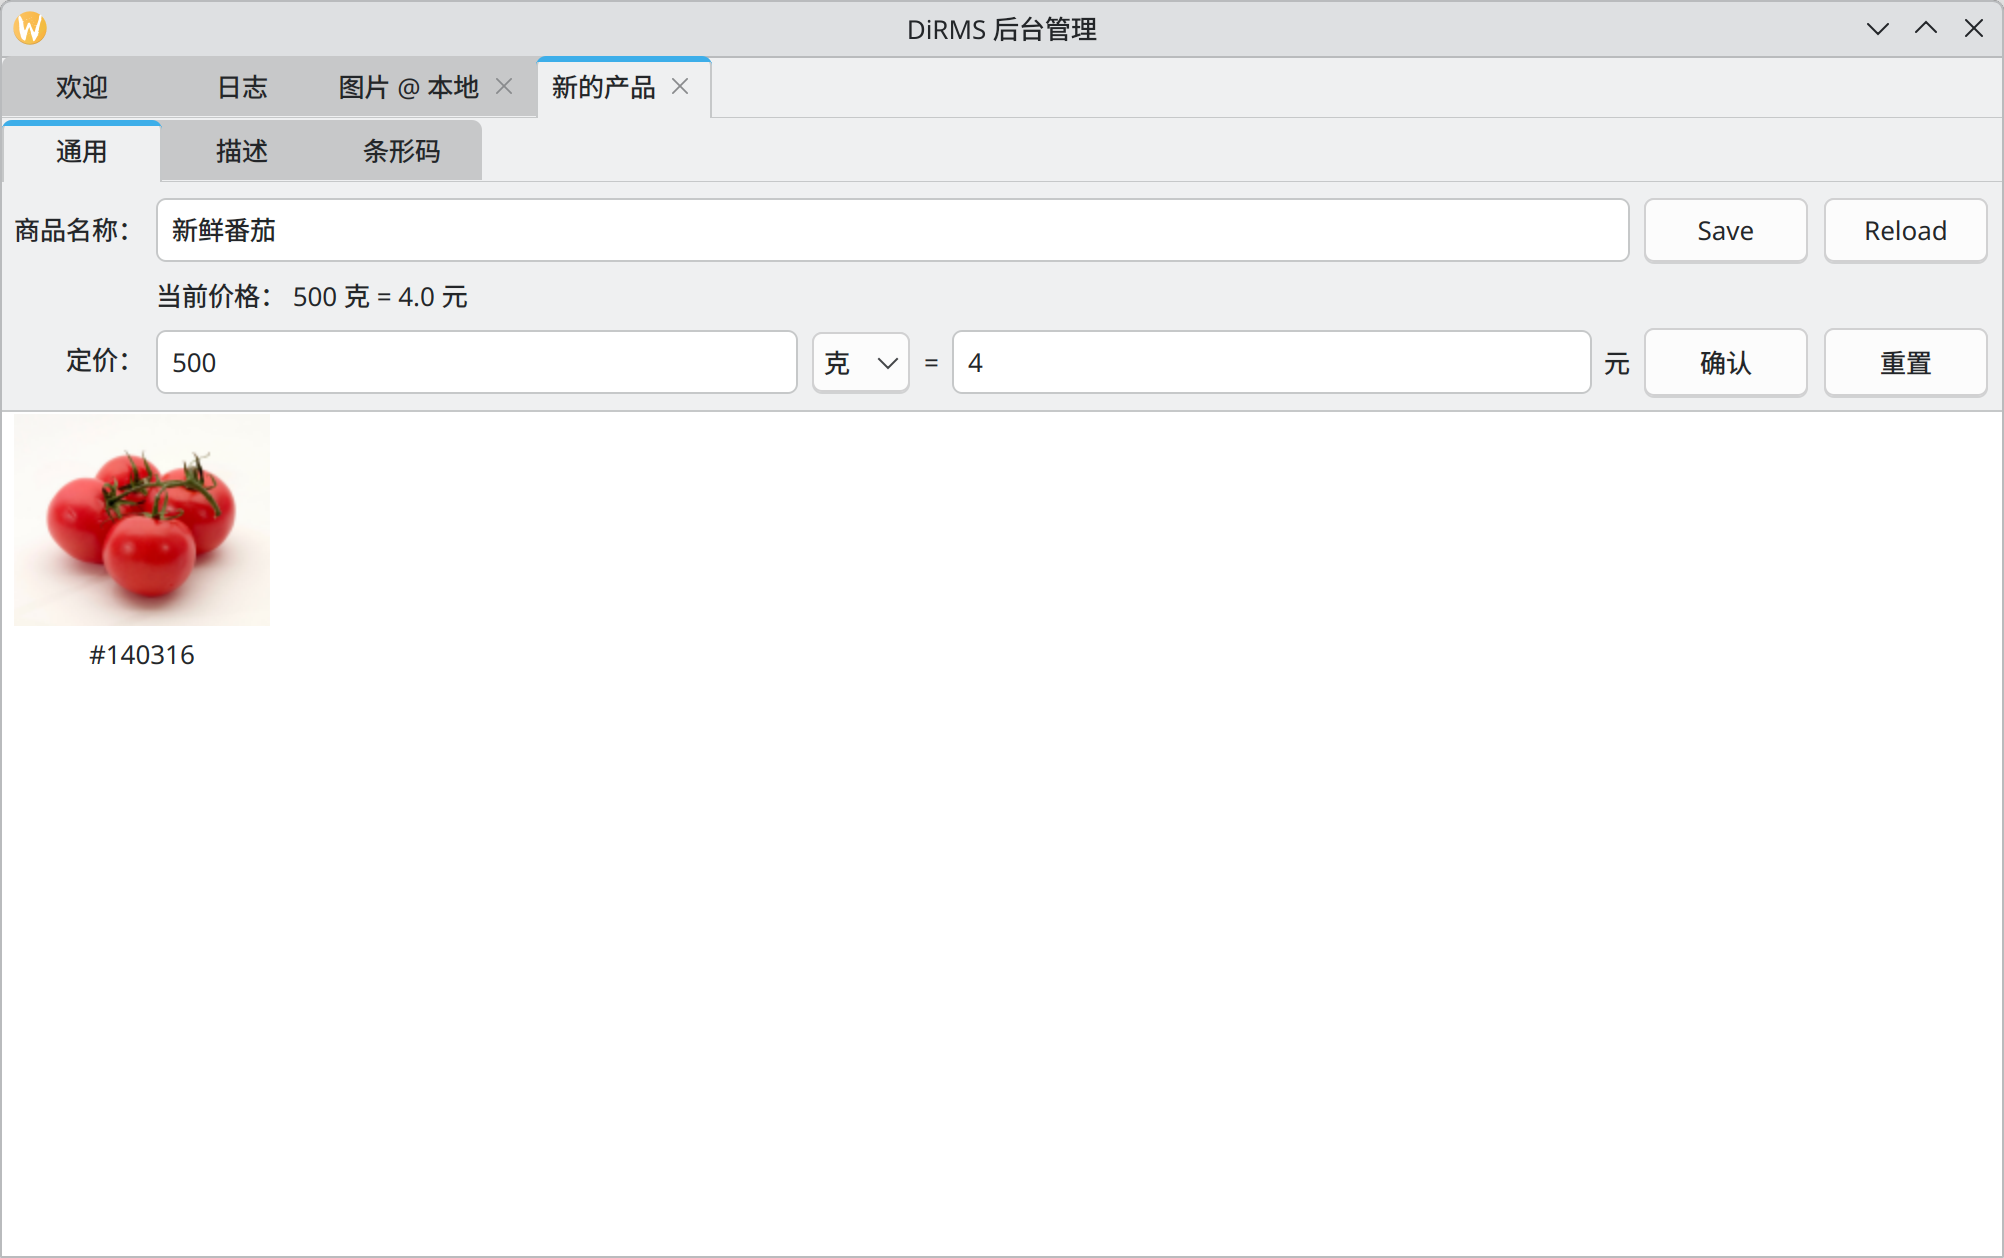
\includegraphics[width=0.3\textwidth]{./exp/rma-prod-add-2.png}}
    \hfill
    \subfloat{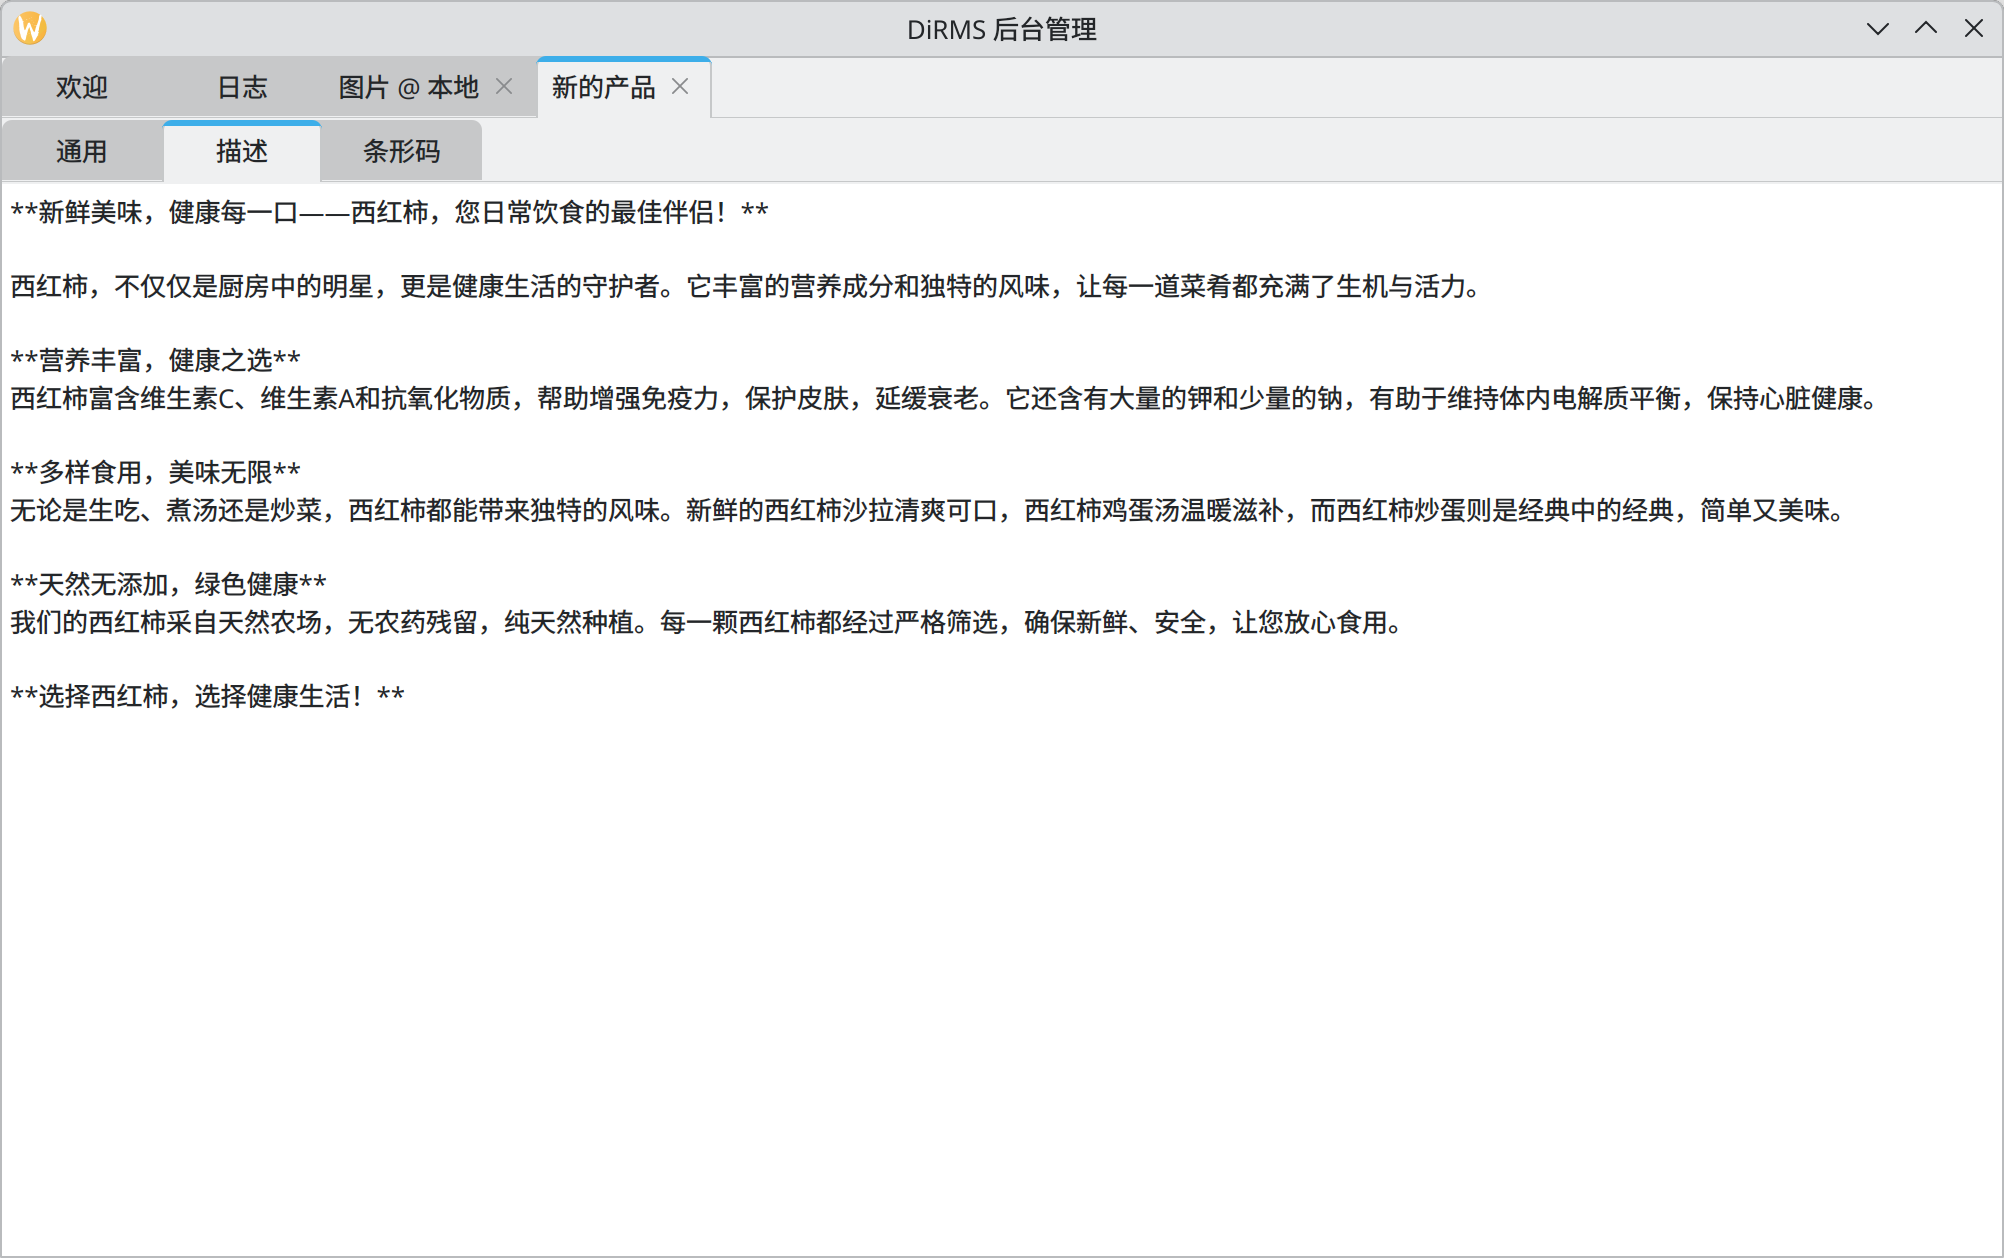
\includegraphics[width=0.3\textwidth]{./exp/rma-prod-add-3.png}}
	\caption{RmAdmin运行效果:添加商品}
	\label{fig:rma-prod-add}
\end{figure}

向系统添加新的商品的界面如图 \ref{fig:rma-prod-add} 所示,其中左图和中图展示了商品基本信息及图片的输入界面。用户可以通过输入框输入商品的名称,定价单位、和单位价格,可以通过下拉菜单选择商品的定价方式,通过点击按钮确认价格修改或保存商品,并且通过画面下侧的空间管理商品图片。用户可以在上文提及的图片管理界面中选择图片,利用右键上下文菜单或快捷键Ctrl-C来复制图片的编号,再通过相似方法(Ctrl-V)来将图片添加到商品,并在保存商品信息时一并存档。右图展示了编辑商品详情的界面,用户可以在空白区域编写商品的详细情况,并随商品基本情况一同保存。

\begin{figure}[htbp]
    \subfloat{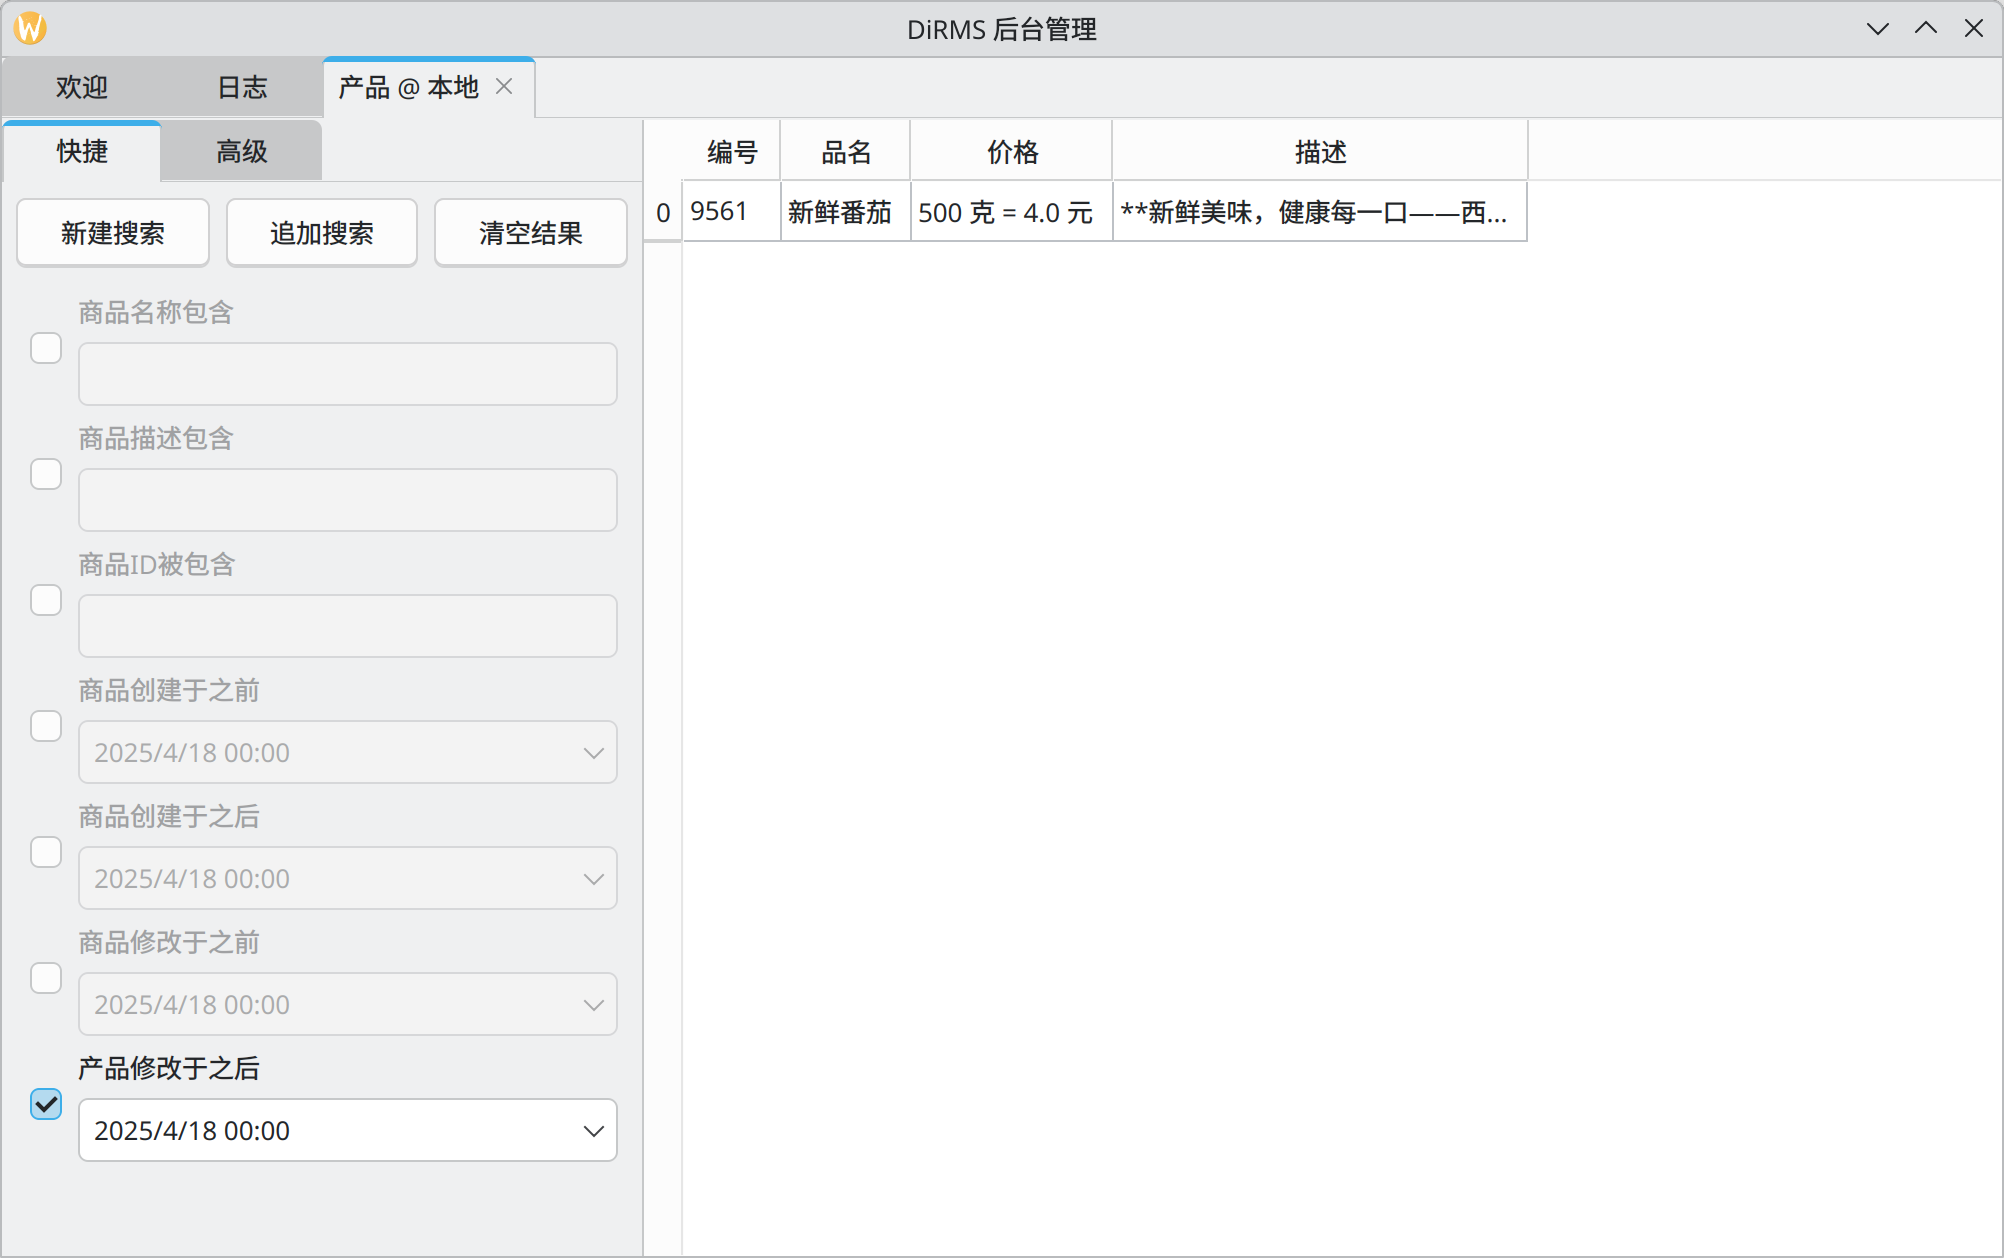
\includegraphics[width=0.3\textwidth]{./exp/rma-prod-as-1.png}}
    \hfill
    \subfloat{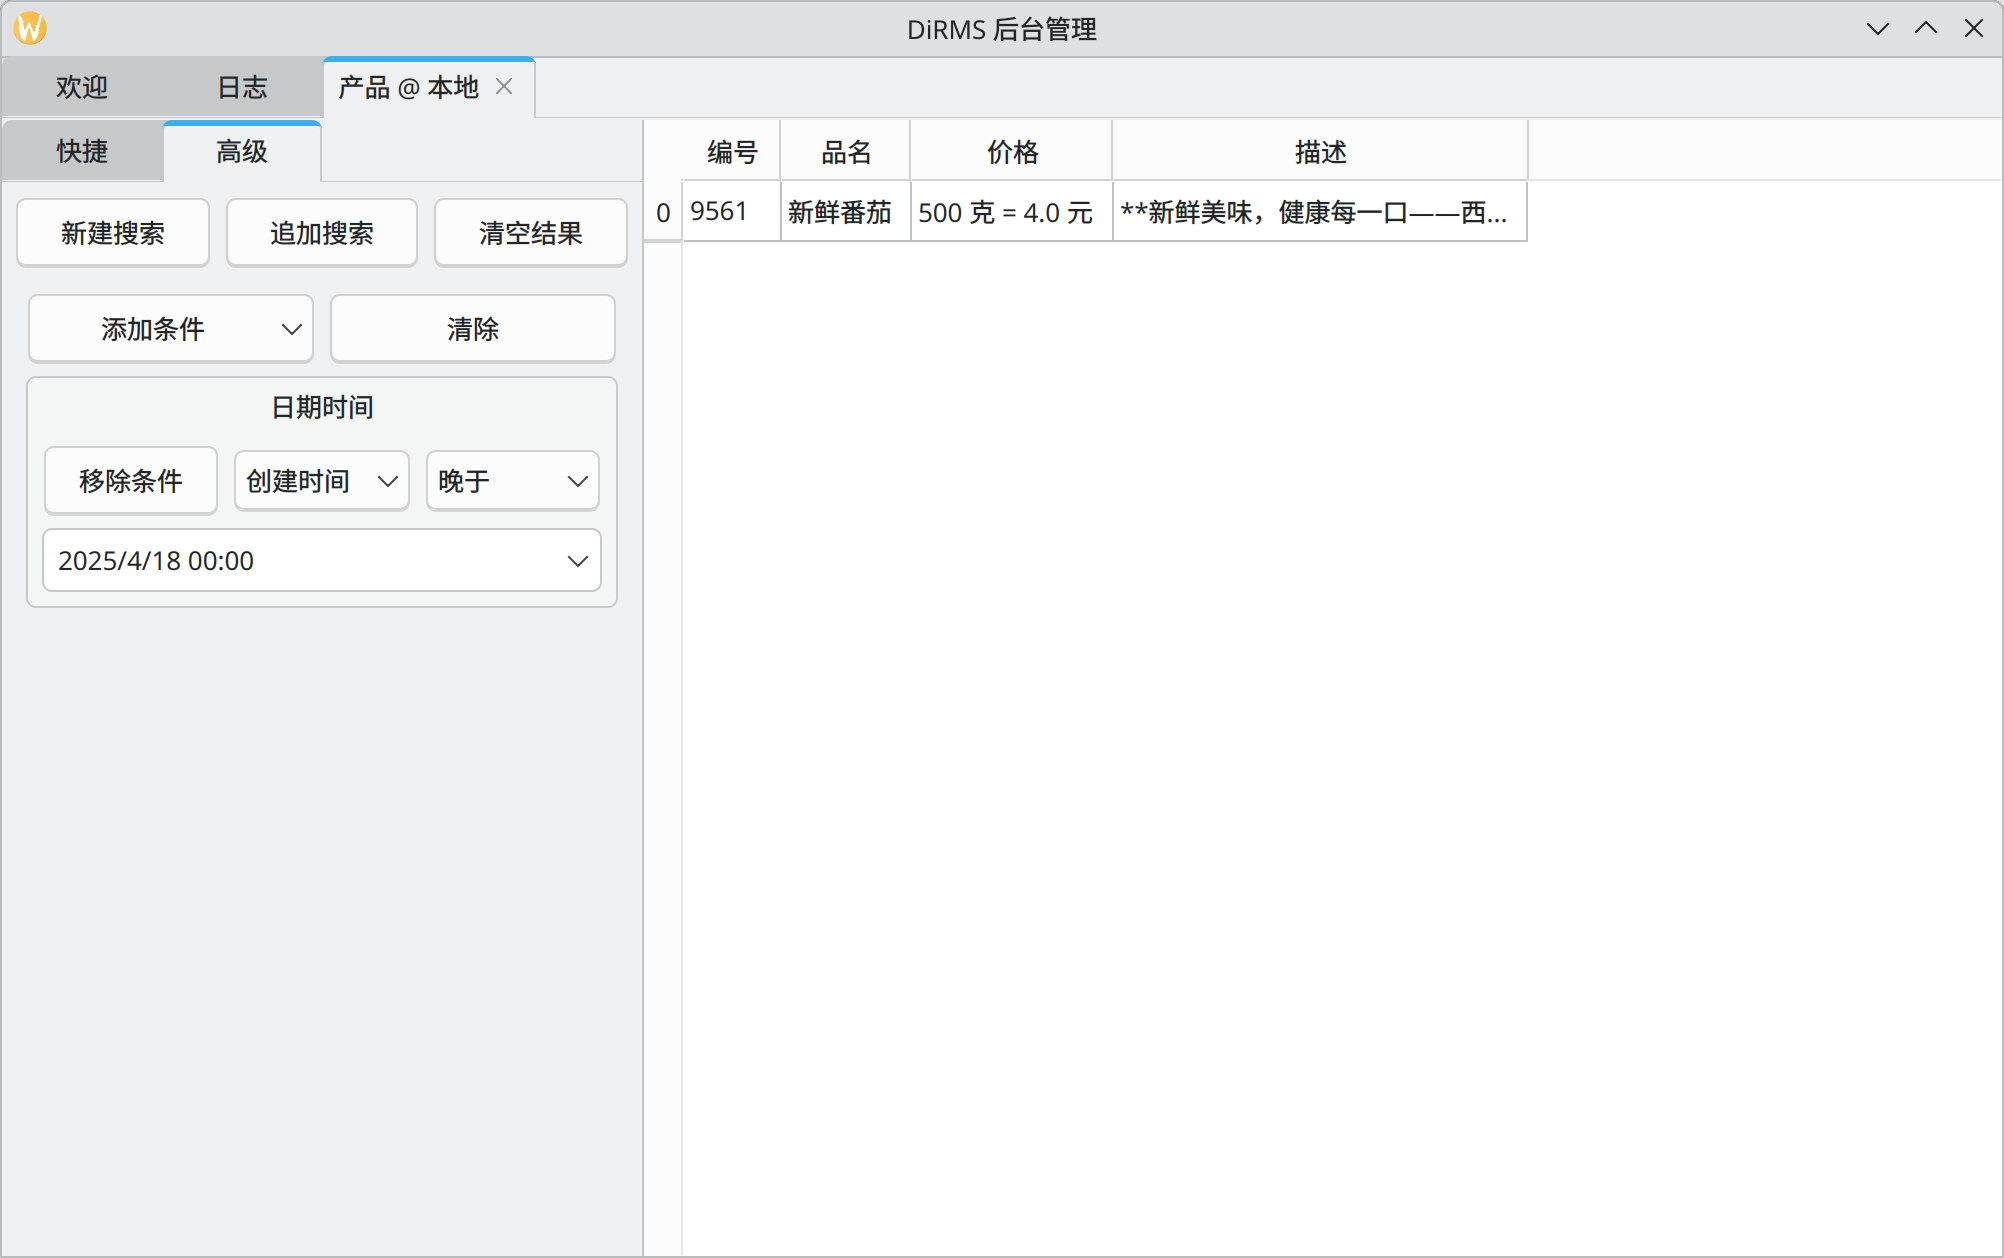
\includegraphics[width=0.3\textwidth]{./exp/rma-prod-as-2.png}}
    \hfill
    \subfloat{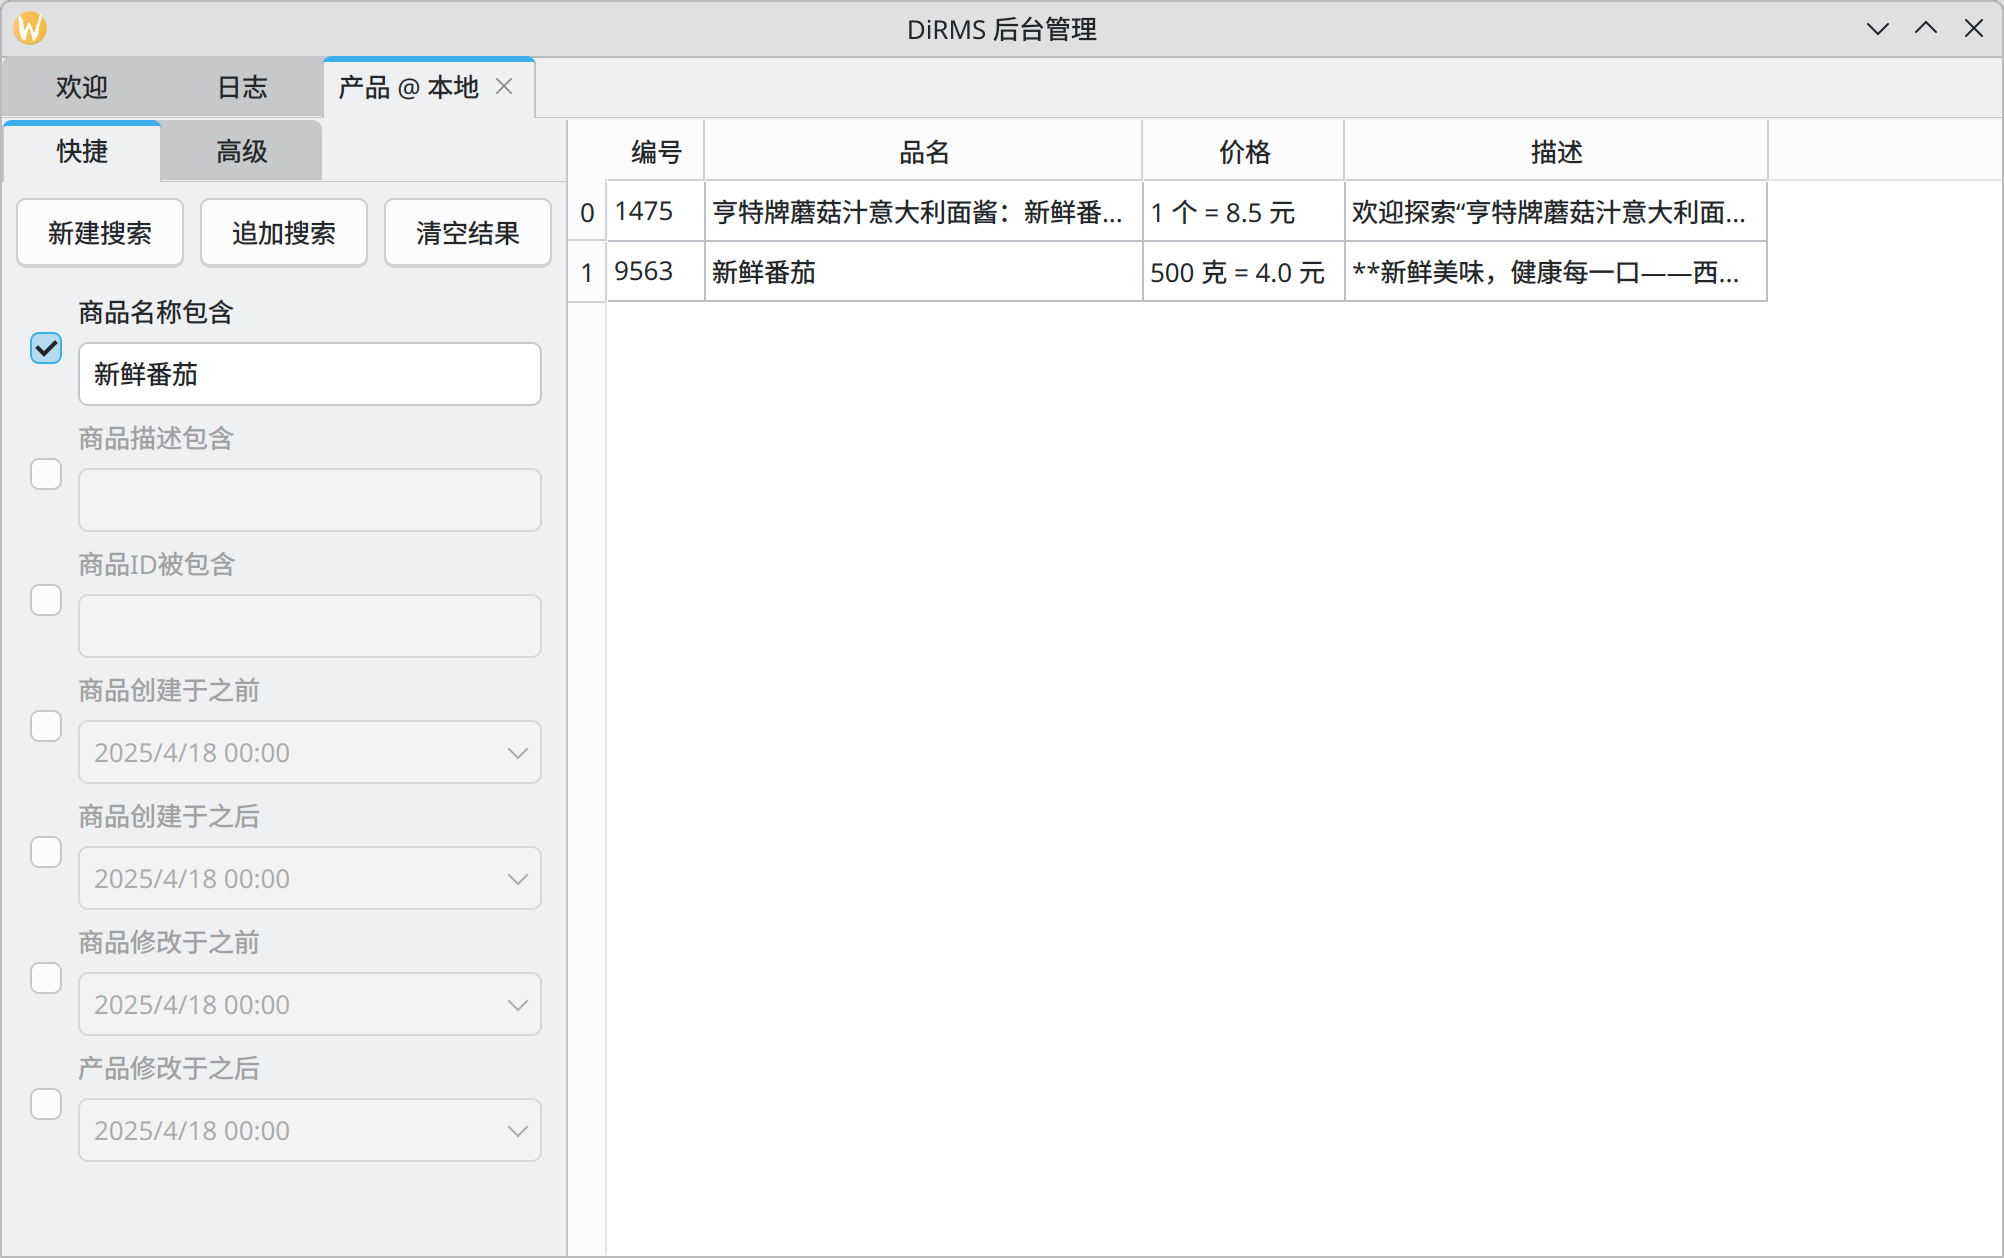
\includegraphics[width=0.3\textwidth]{./exp/rma-prod-as-3.png}}
	\caption{RmAdmin运行效果:商品高级搜索}
	\label{fig:rma-prod-as}
\end{figure}

应用程序对商品有较图片更加复杂的搜索特性。如图 \ref{fig:rma-prod-as} 所示,用户可以根据需要在快速搜索和高级搜索方式中选择,其中快速搜索包含了一般营业场景中较为常用的商品名称、描述、创建和修改时间等条件的合理判断方式,用户可以通过和高级搜索图片一样的方式启用或停用条件、修改条件内容,最后通过上侧的按钮来进行实际的查询操作。

同样,用户可以选择进行高级查询。高级查询界面如图 \ref{fig:rma-prod-as} 中中间子图所示,用户可以通过画面左侧的图形化查询设计工具设计任意复杂程度的,可能包括组合条件和反条件的复杂查询,可以充分满足用户的任何精细化的商品查询需要。

\begin{figure}[htbp]
    \subfloat{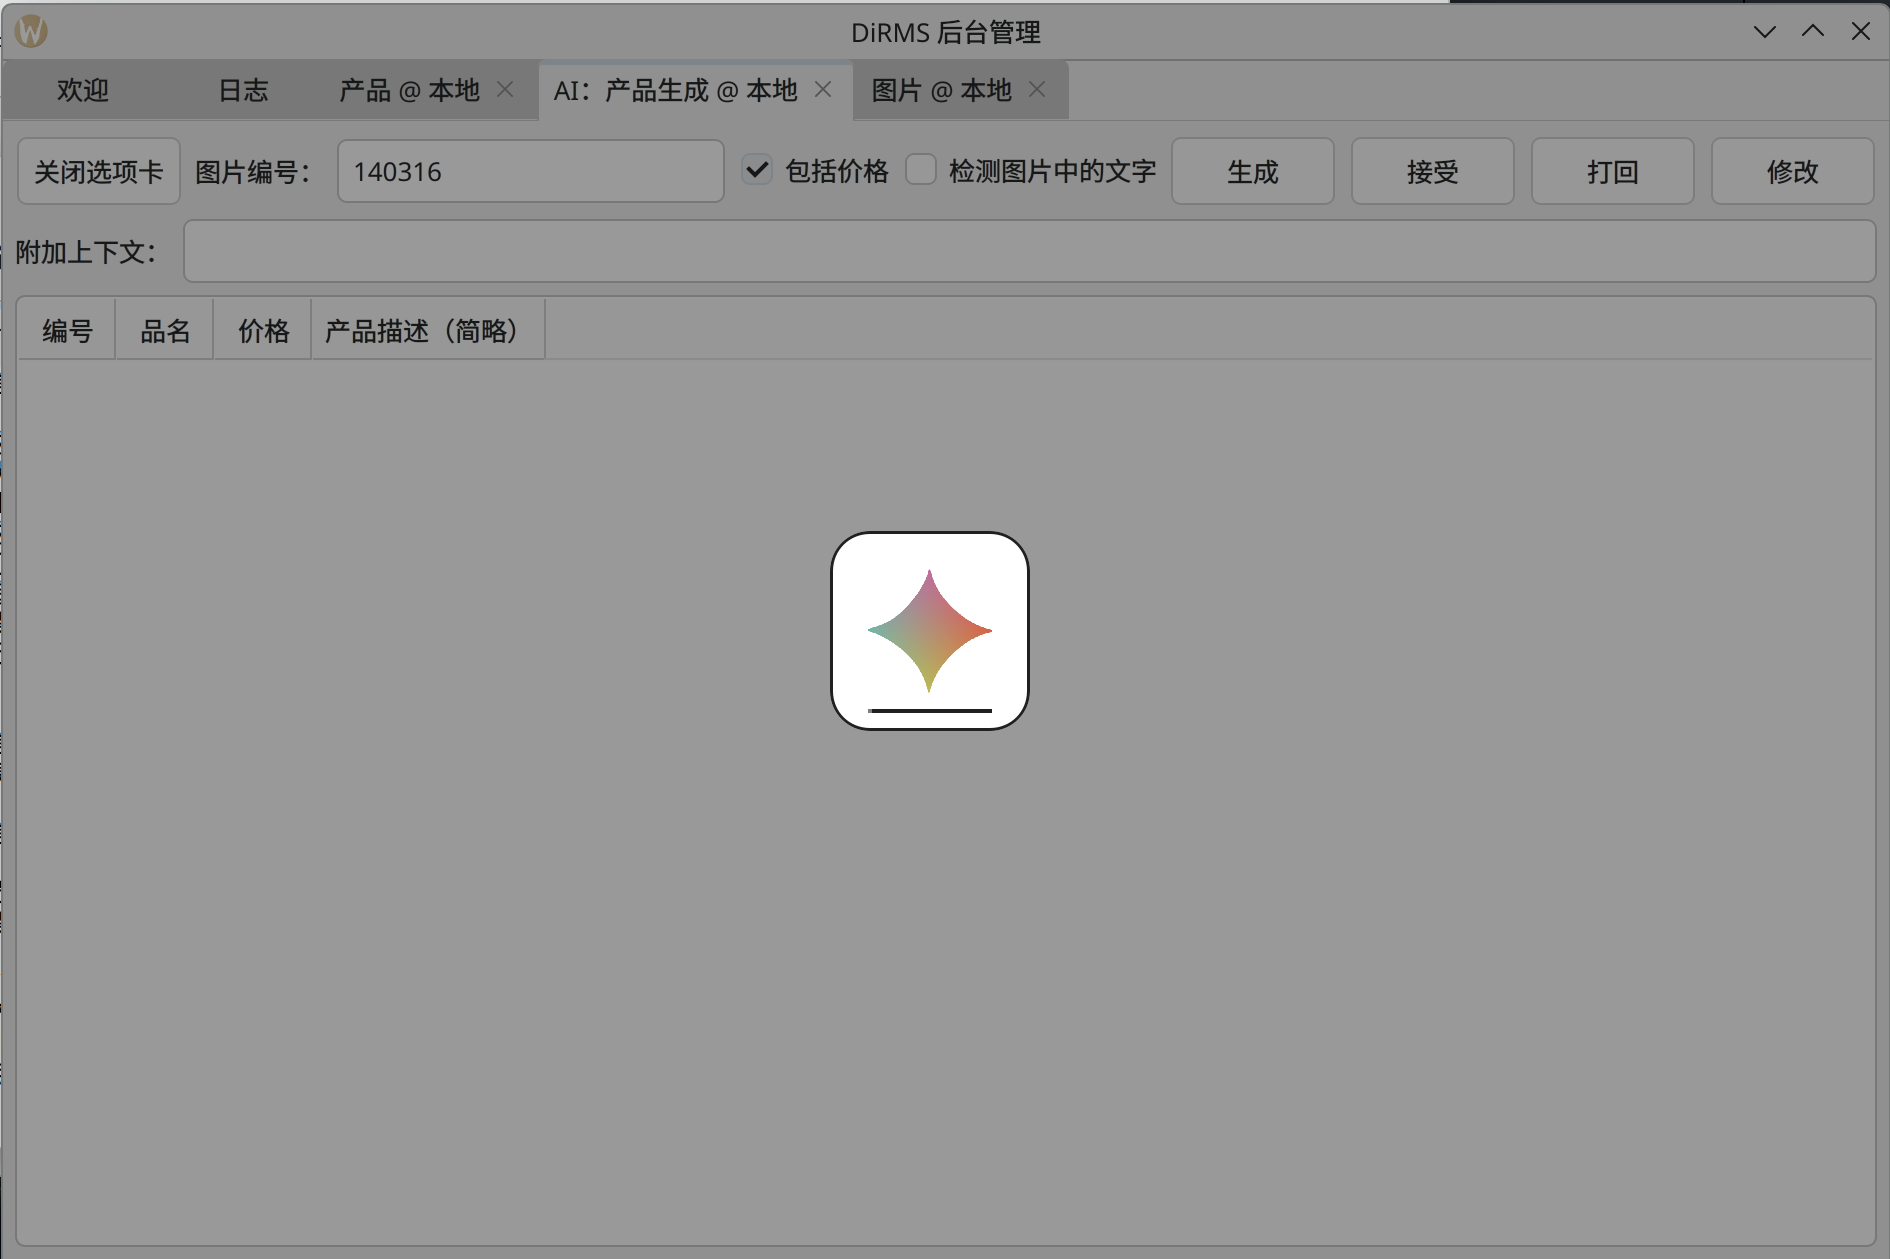
\includegraphics[width=0.3\textwidth]{./exp/rma-ai-bulk-1.png}}
    \hfill
    \subfloat{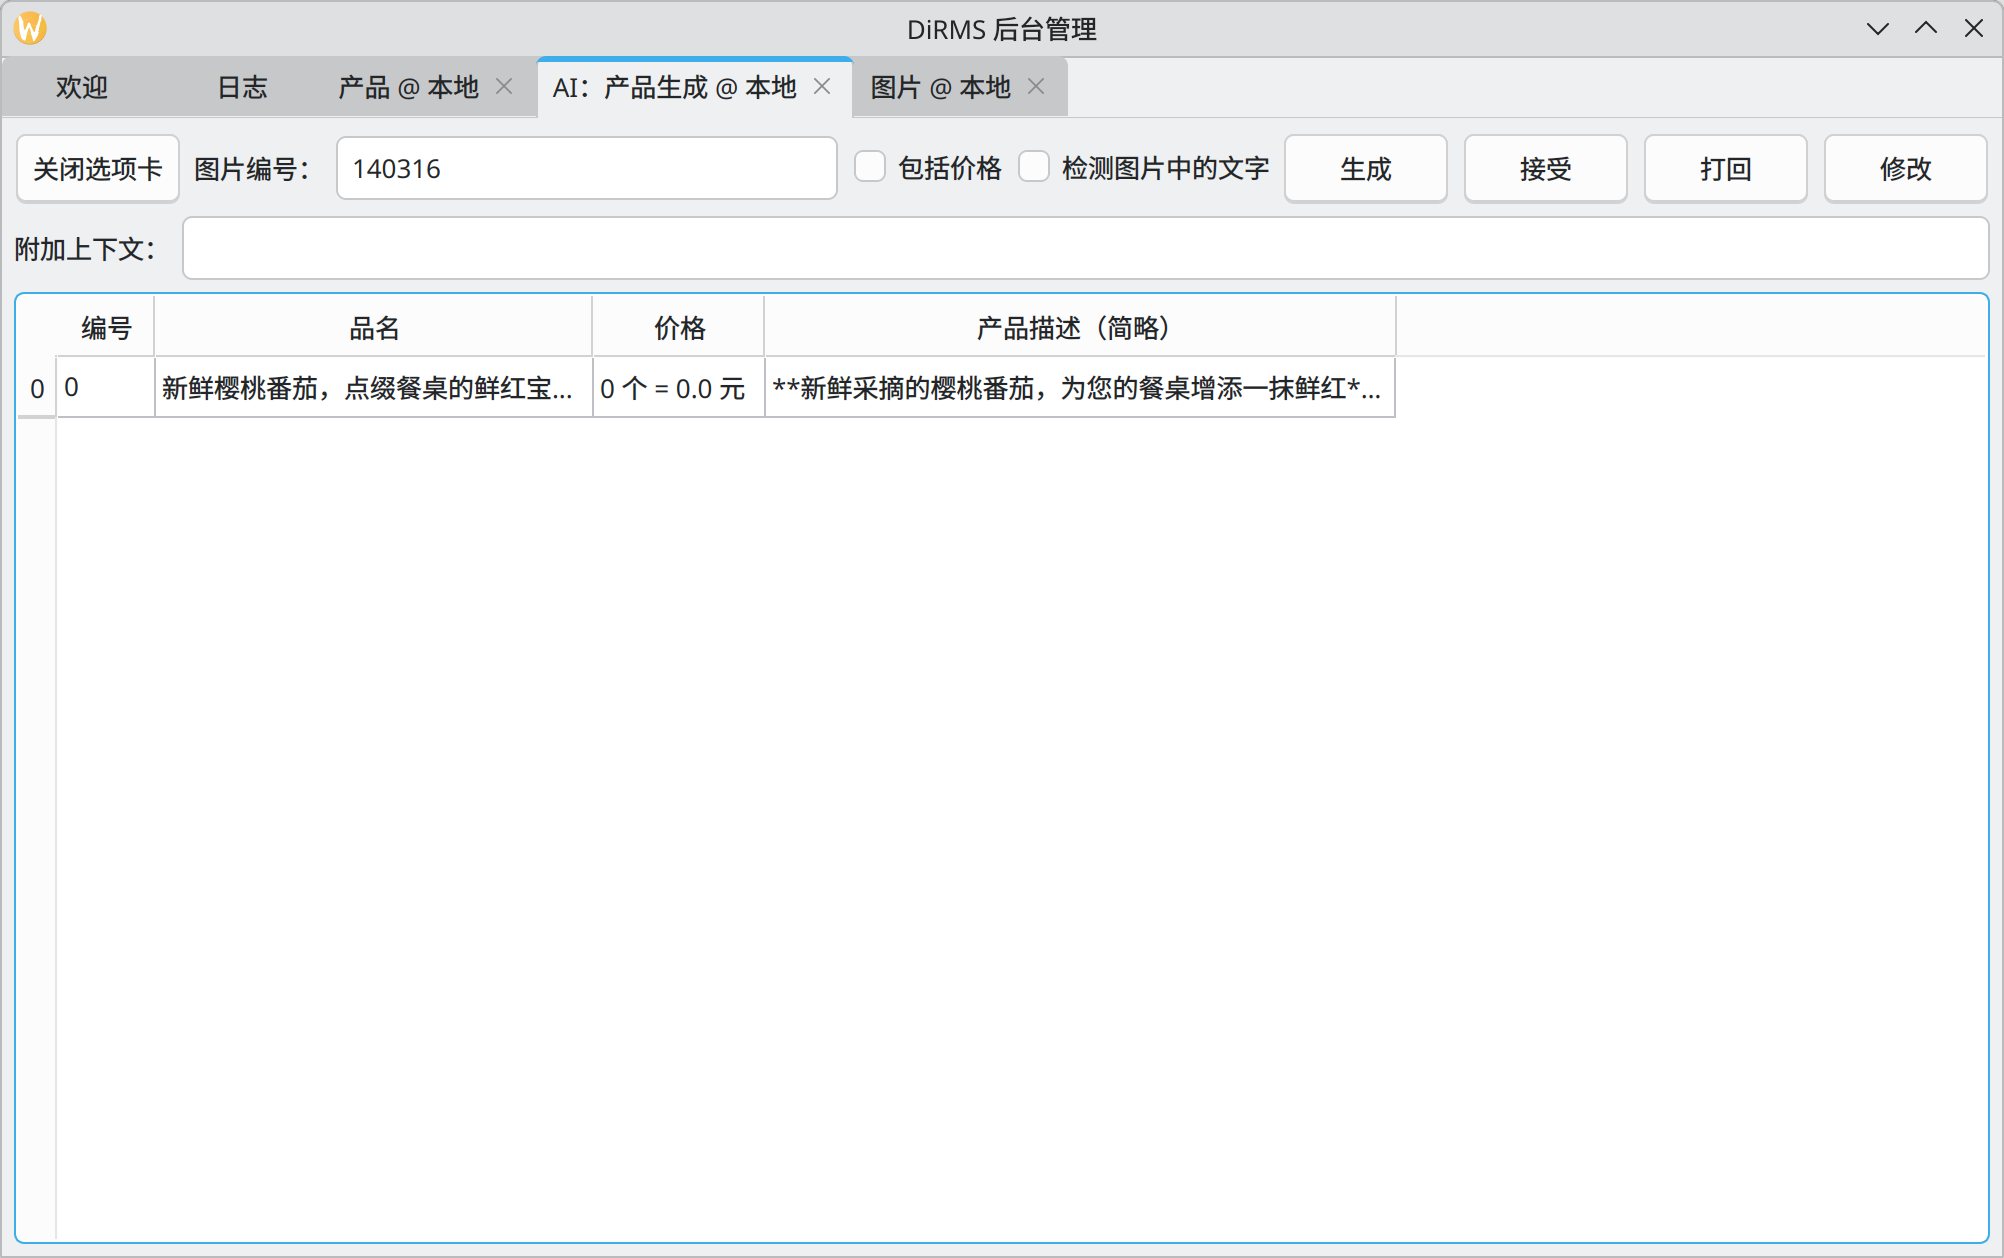
\includegraphics[width=0.3\textwidth]{./exp/rma-ai-bulk-2.png}}
    \hfill
    \subfloat{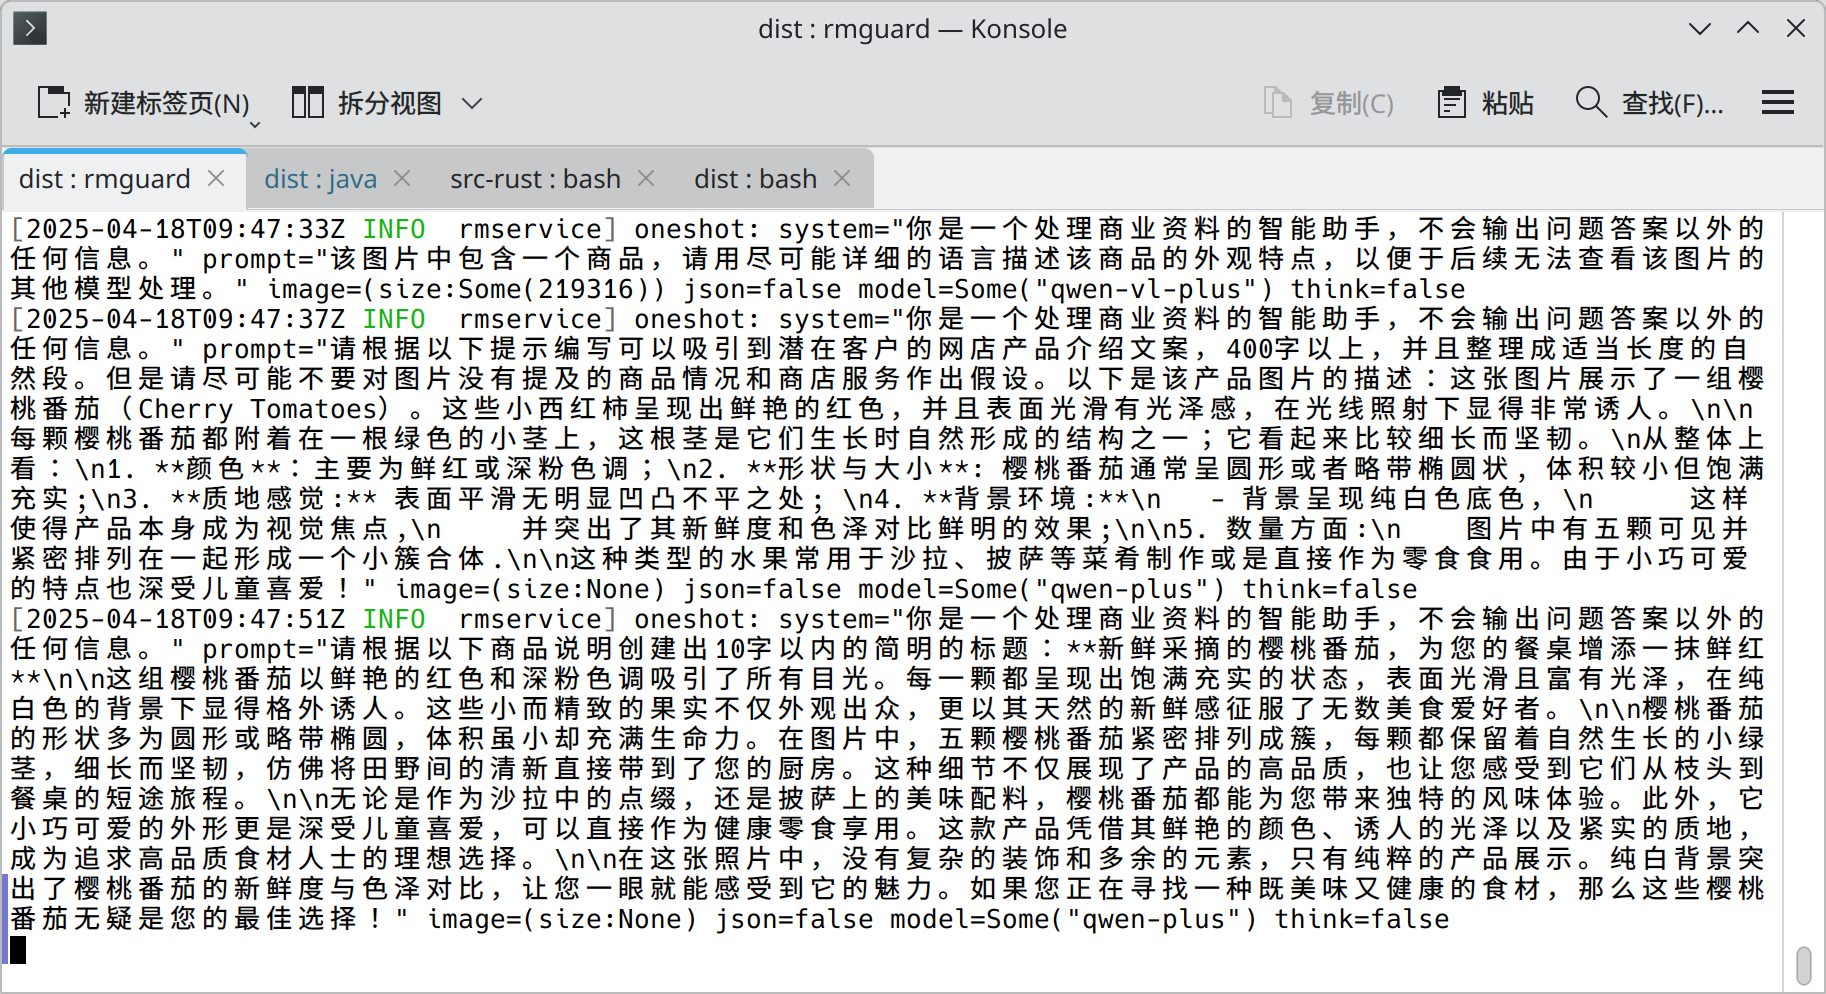
\includegraphics[width=0.3\textwidth]{./exp/rma-ai-bulk-3.png}}
	\caption{RmAdmin运行效果:批量AI商品生成}
	\label{fig:rma-ai-bulk}
\end{figure}

如图所示在AI批量产品生成界面,用户可以通过提供一系列图片(编号)来利用AI根据制定的图片进行产品信息(名称、描述和可选的价格)编写。在AI相关操作进行的过程中,如左图所示的动画将会持续播放以提供界面反馈。生成的结果将会在如中图下侧的表格中展示,用户可以根据生成结果的简略版本决定是否接受生成结果,也可以通过将条目打开为新商品,并进行手工修正及其他优化工作。

\begin{figure}[htbp]
    \subfloat{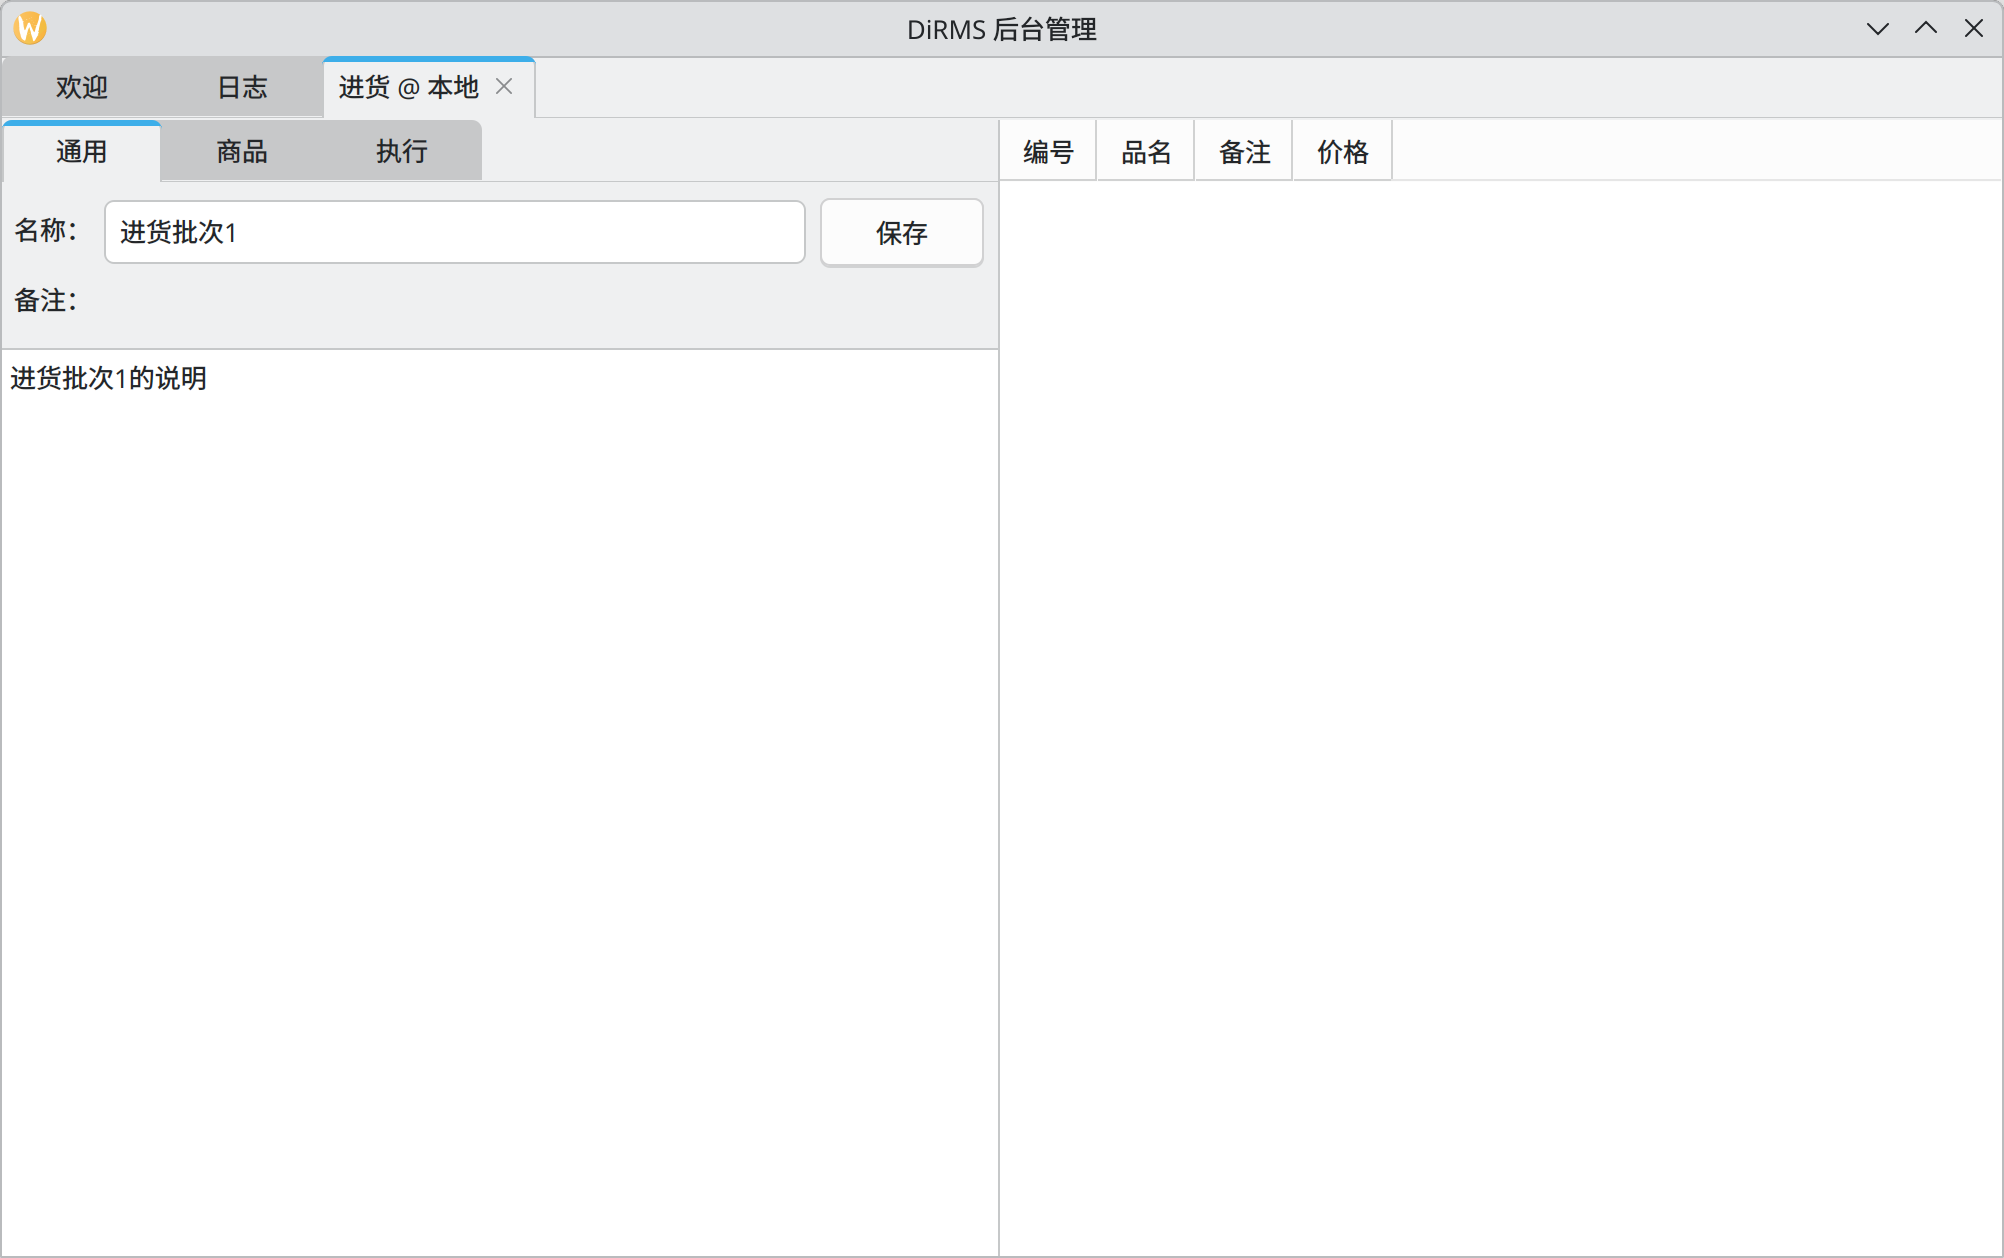
\includegraphics[width=0.3\textwidth]{./exp/rma-ir-plan-1.png}}
    \hfill
    \subfloat{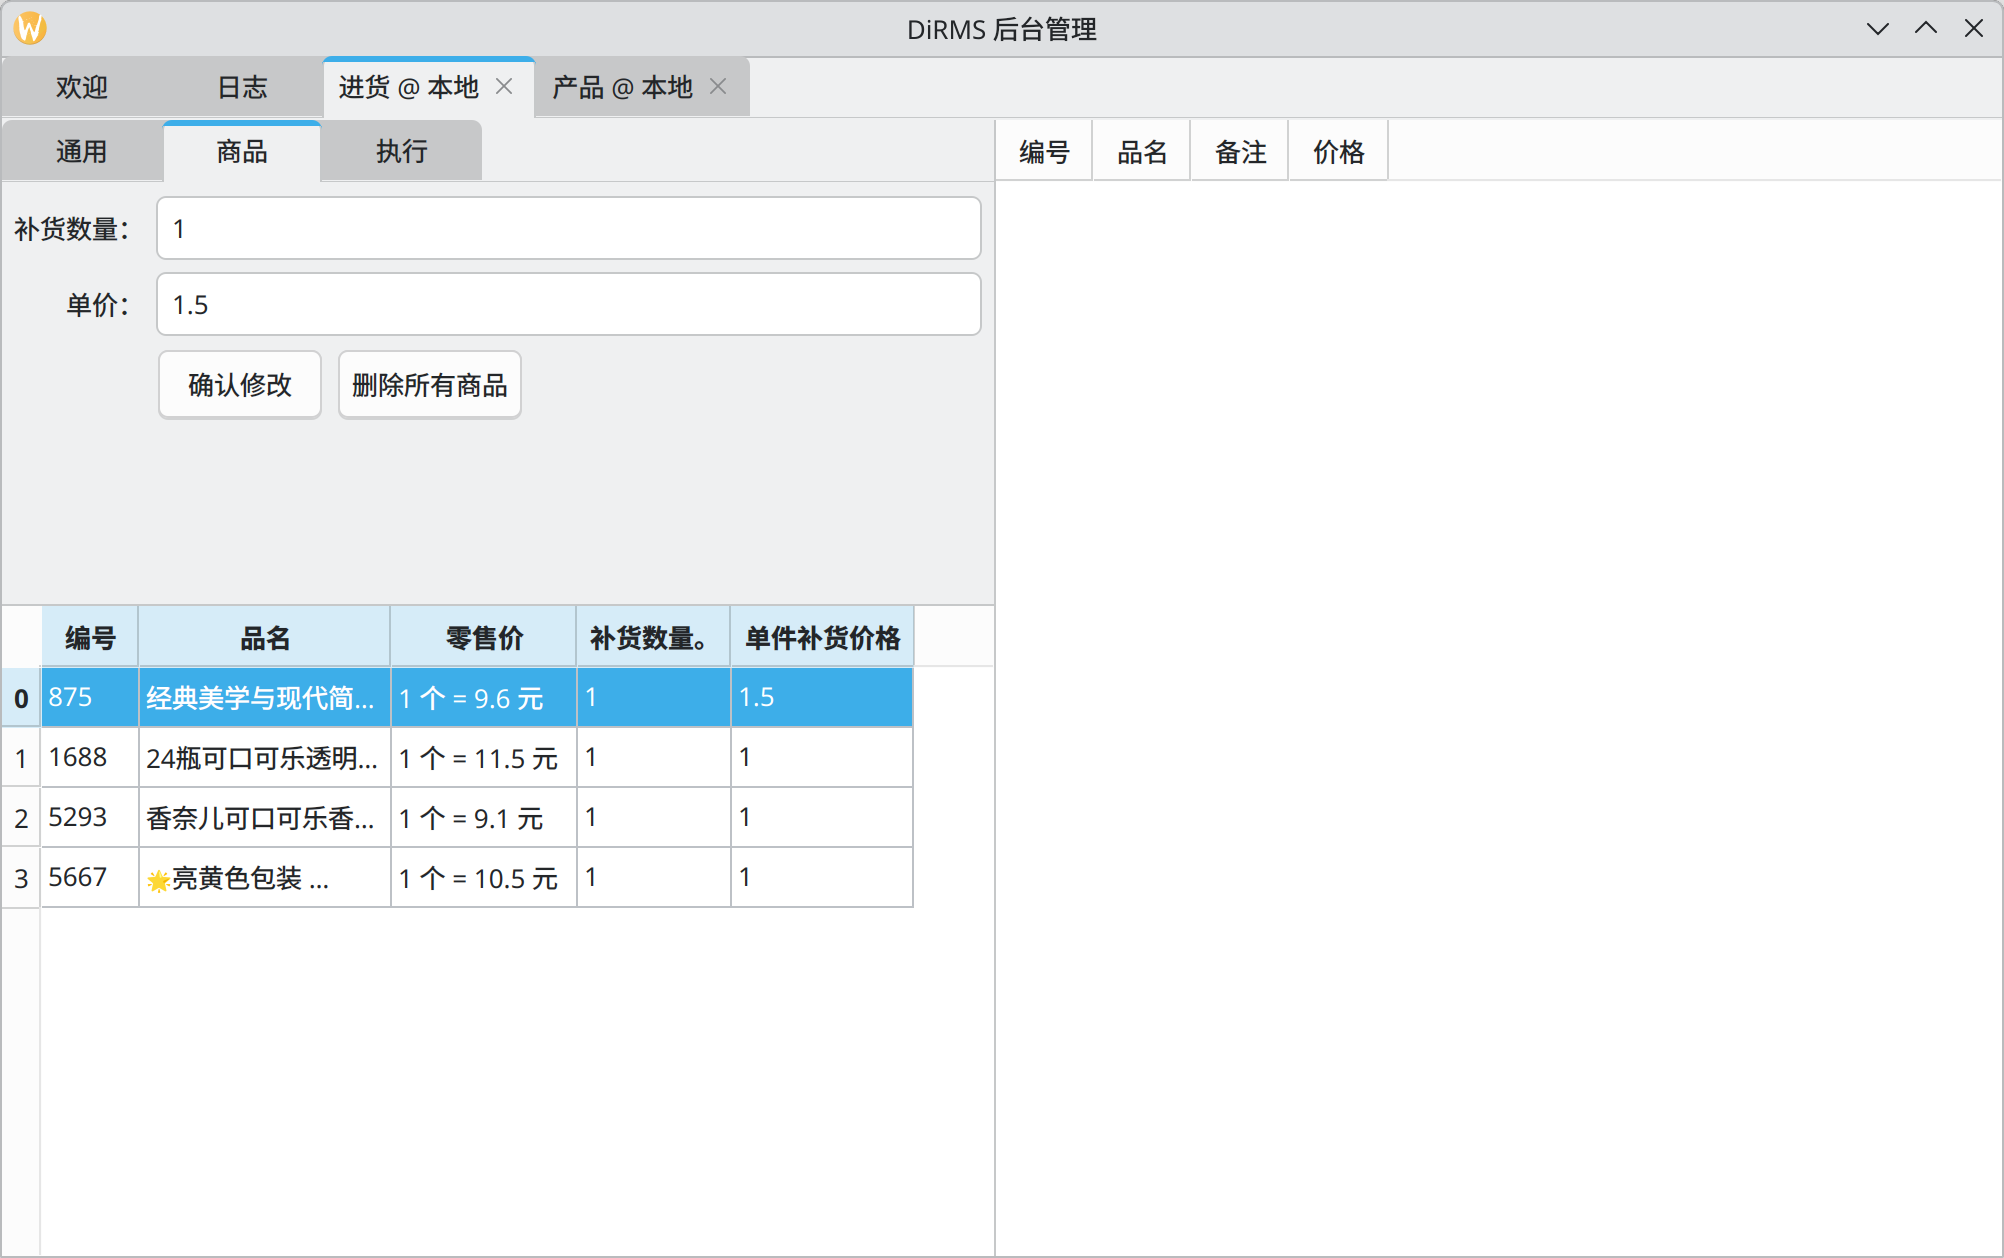
\includegraphics[width=0.3\textwidth]{./exp/rma-ir-plan-2.png}}
    \hfill
    \subfloat{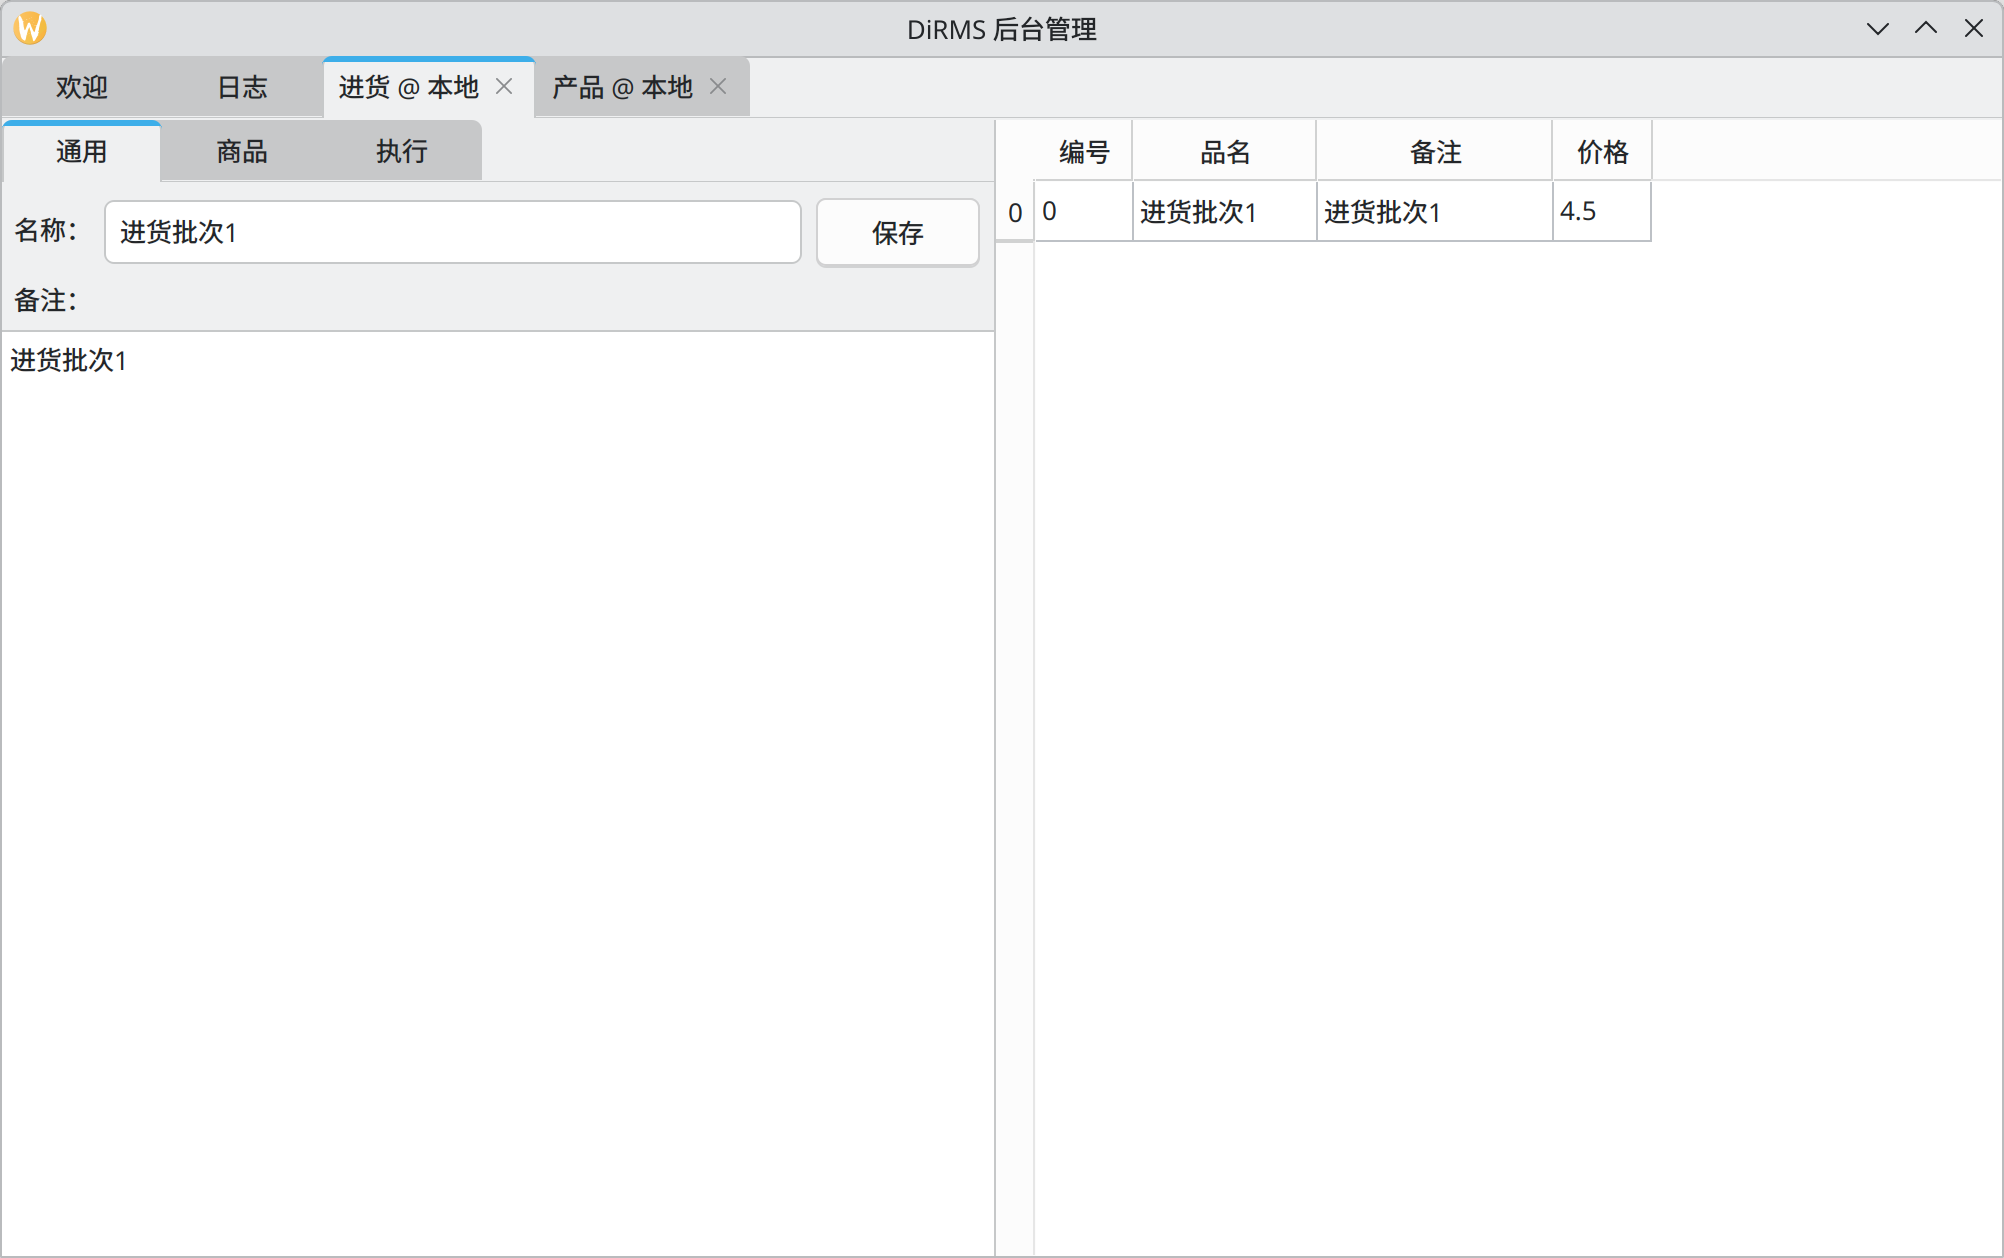
\includegraphics[width=0.3\textwidth]{./exp/rma-ir-plan-3.png}}
	\caption{RmAdmin运行效果:制定进货计划}
	\label{fig:rma-ir-plan}
\end{figure}

用户可以通过如图 \ref{fig:rma-ir-plan} 所示的界面进行进货计划的管理和执行操作。画面左侧展示了单个进货计划(或新计划)的细节,右侧展示了可选地全部计划。在画面左侧的第一个标签页中用户可以修改进货计划名字和描述,在第二个标签页中用户可以通过粘贴(与图片管理同理,从商品管理界面搜索并复制的)商品编号来添加进货商品,并通过上侧的输入框来修改选择的商品项的(每一次)进货量和(每一单位)进货价格。

\begin{figure}[htbp]
	\centering
	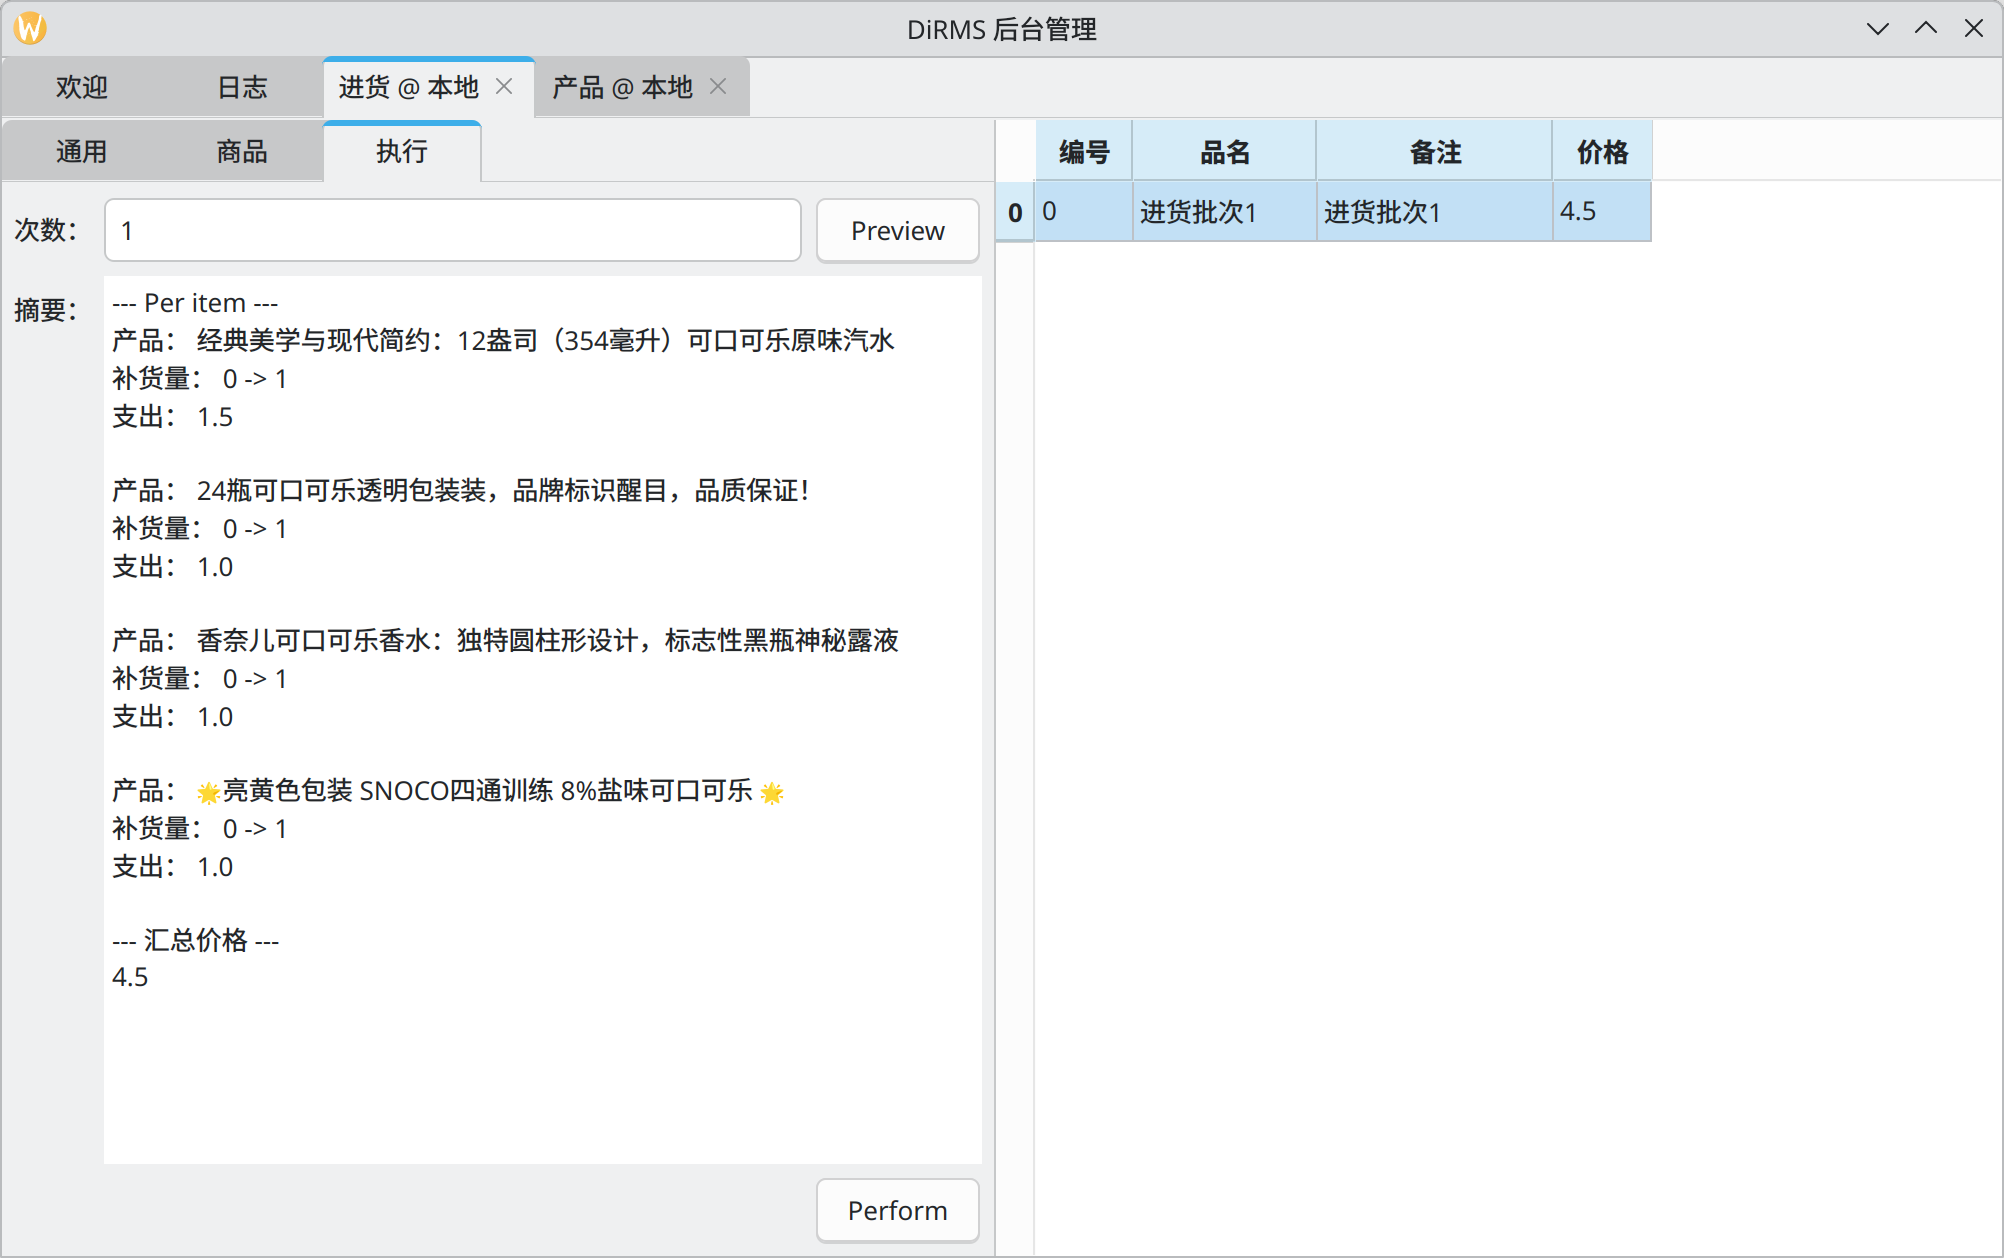
\includegraphics[width=0.8\textwidth]{./exp/rma-ir-exec-1.png}
	\caption{RmAdmin运行效果:执行进货计划}
	\label{fig:rma-ir-exec-1}
\end{figure}

利用第三个标签页“执行”,用户可以制定进货计划的执行次数并预览进货计划的执行摘要。通过点击“执行”按钮指定进货计划将会被按指定次数执行。

\begin{figure}[htbp]
    \subfloat{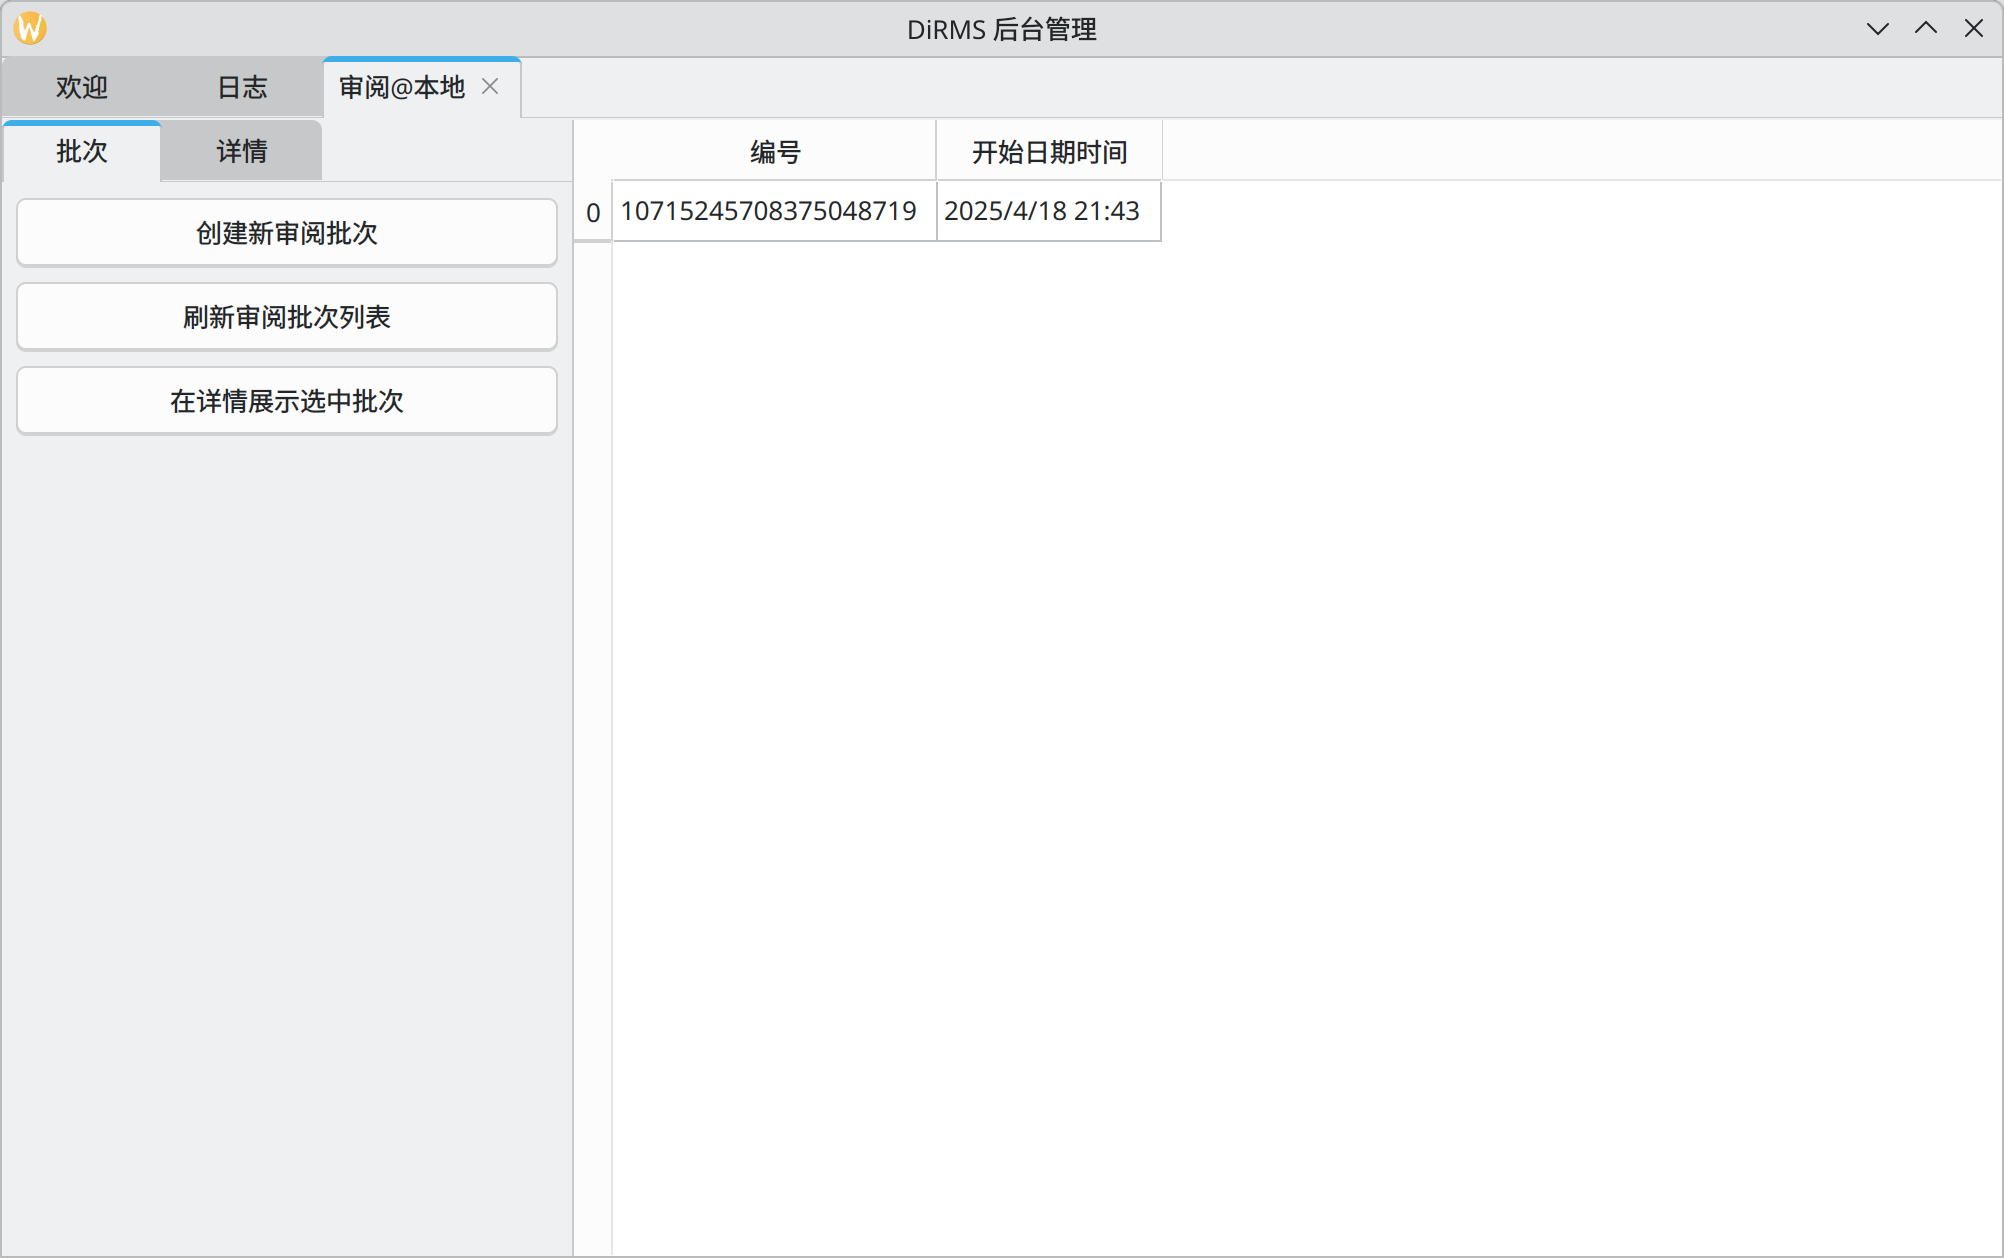
\includegraphics[width=0.45\textwidth]{./exp/rma-audit-1.png}}
    \hfill
    \subfloat{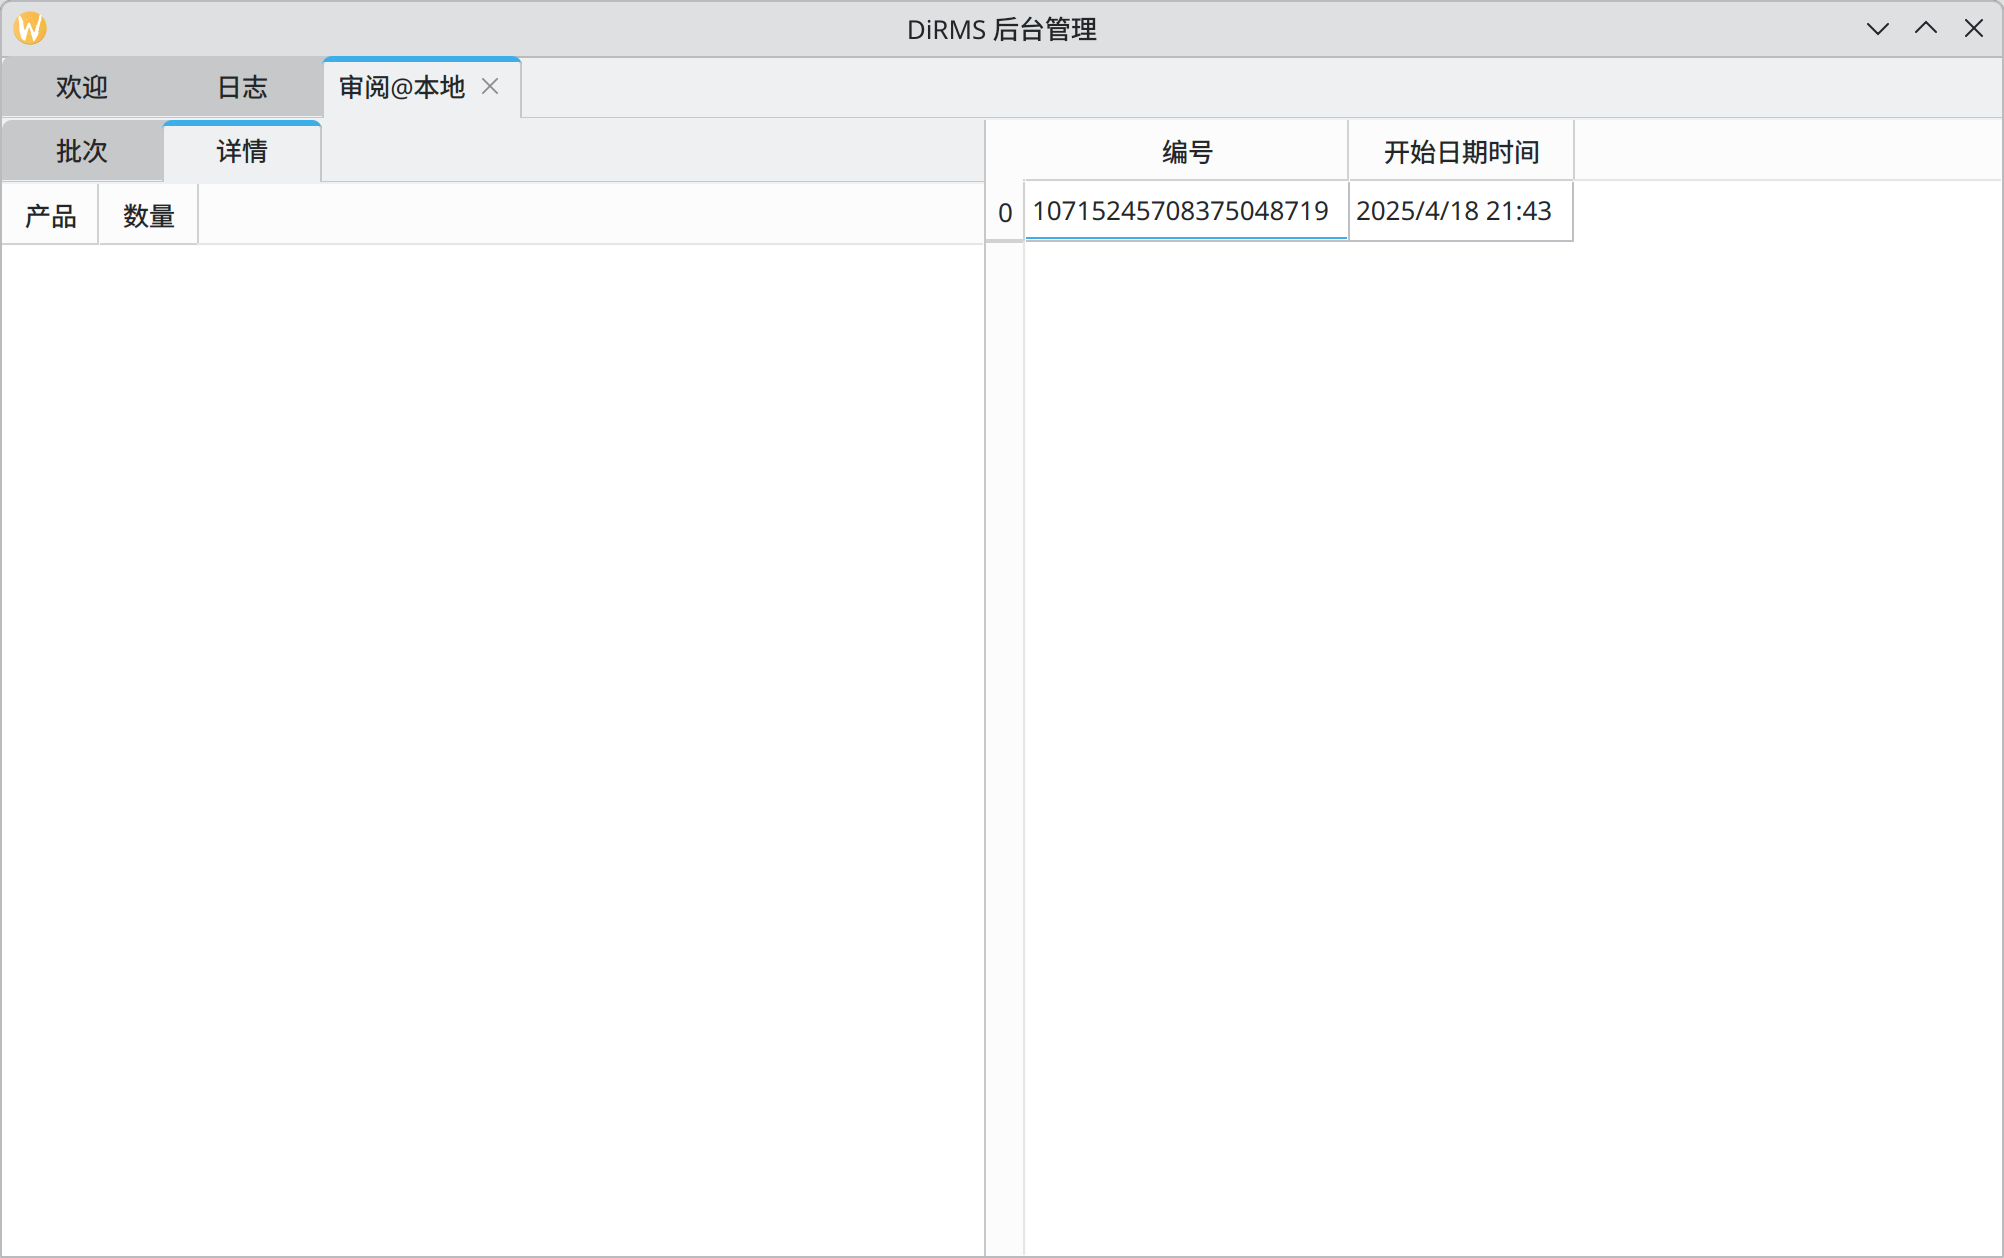
\includegraphics[width=0.45\textwidth]{./exp/rma-audit-2.png}}
	\caption{RmAdmin运行效果:库存审阅}
	\label{fig:rma-audit}
\end{figure}

用户可以通过如图 \ref{fig:rma-audit} 所示的界面进行库存审阅批次的创建、删除和管理。值得注意的是,审阅批次因为其较短的时效性并不存储在数据库中,而是由RmService服务器直接进行管理,任何审阅批次都将被指定一个随机的(64位)编号并被记录其开始时间。

\begin{figure}[htbp]
	\centering
	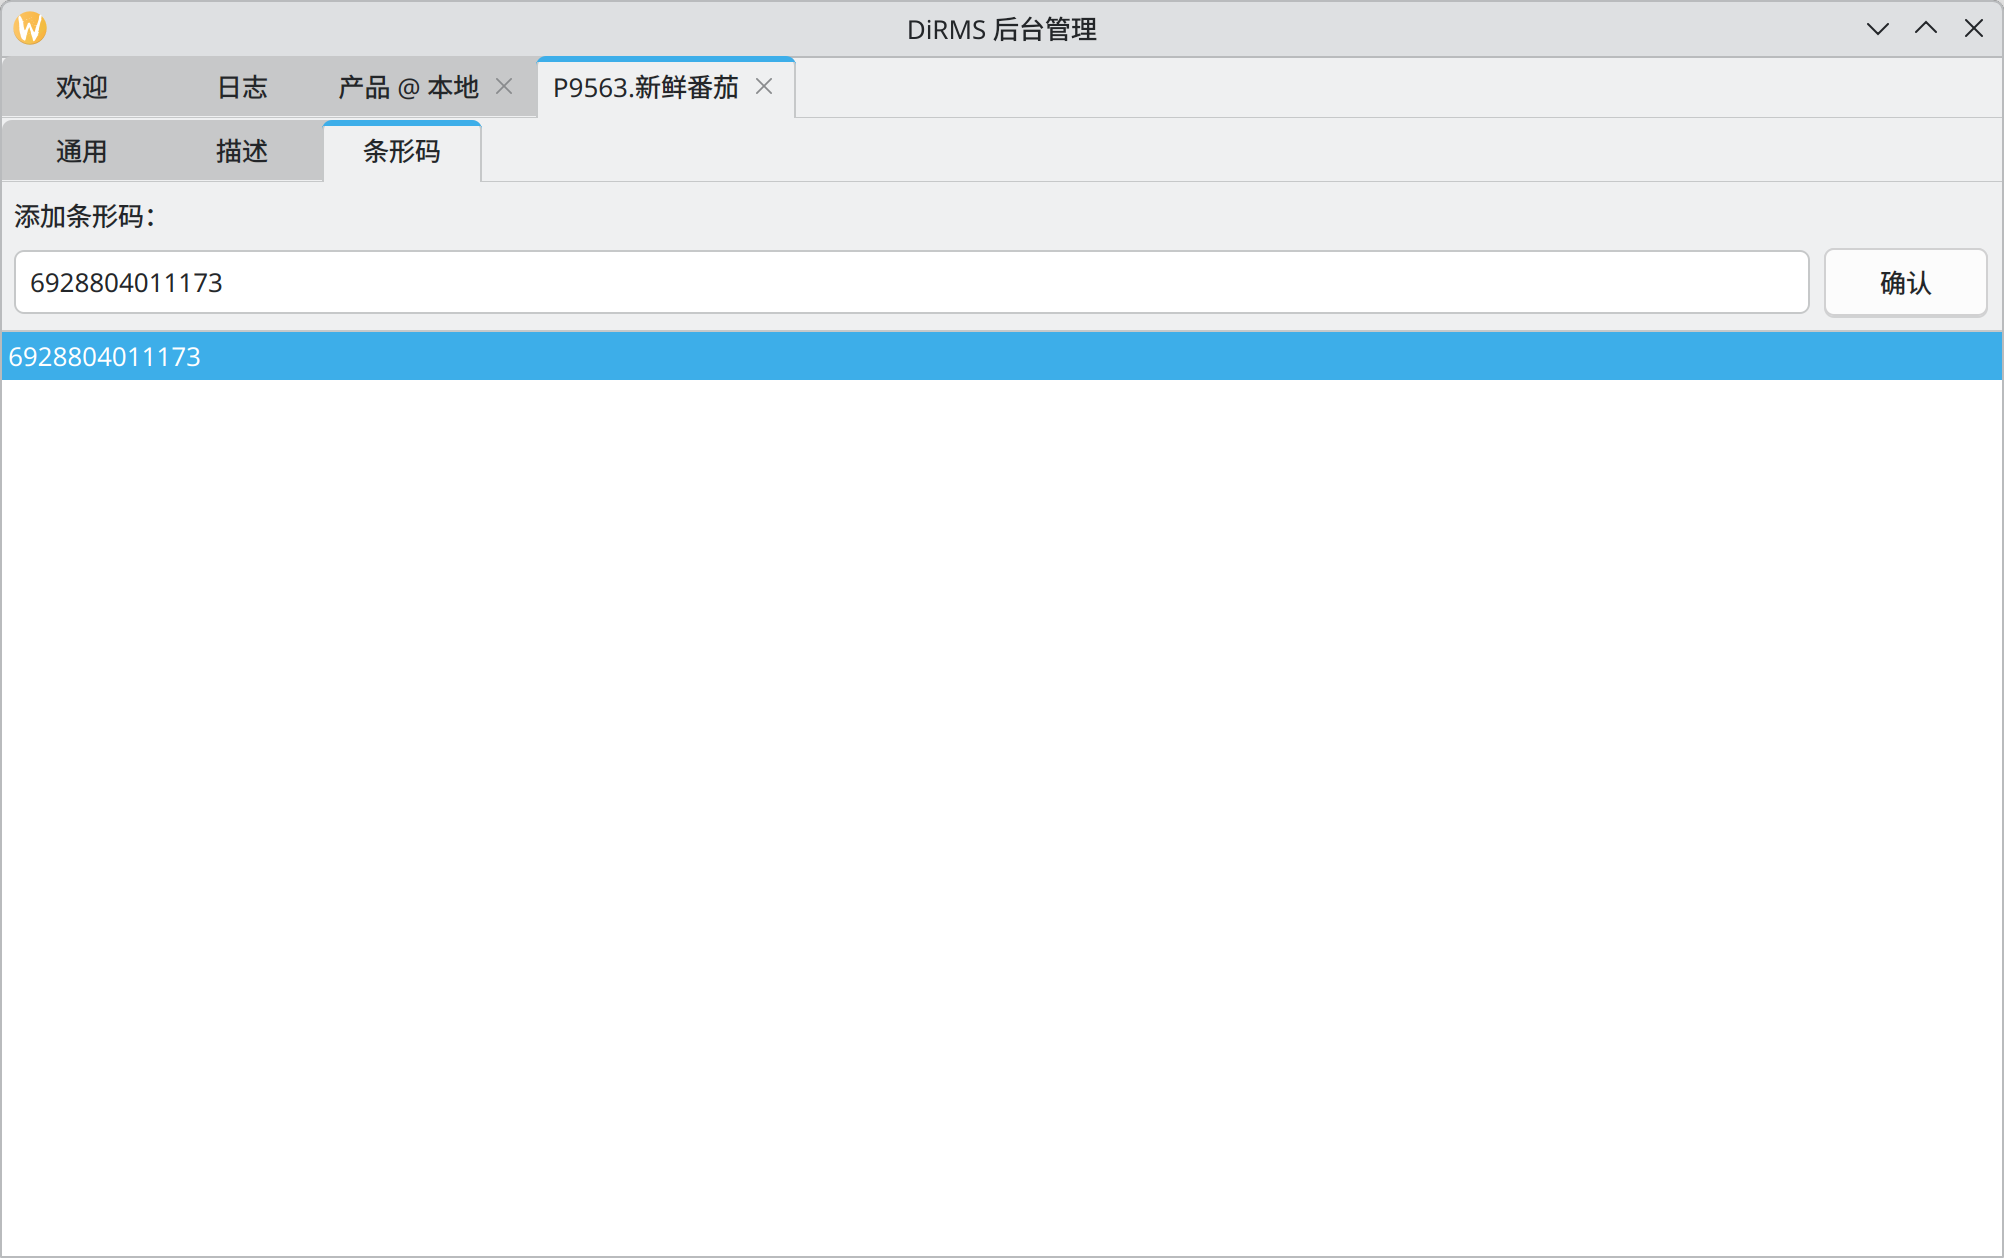
\includegraphics[width=0.8\textwidth]{./exp/rma-bc.png}
	\caption{RmAdmin运行效果:条码管理}
	\label{fig:rma-bc}
\end{figure}

利用如图 \ref{fig:rma-bc} 所示的(商品编辑界面中的)条形码管理选项卡,用户可以为商品指定一个或多个条形码。该条形码其后可被用于结算过程中的商品的标识。

\begin{figure}[htbp]
	\centering
	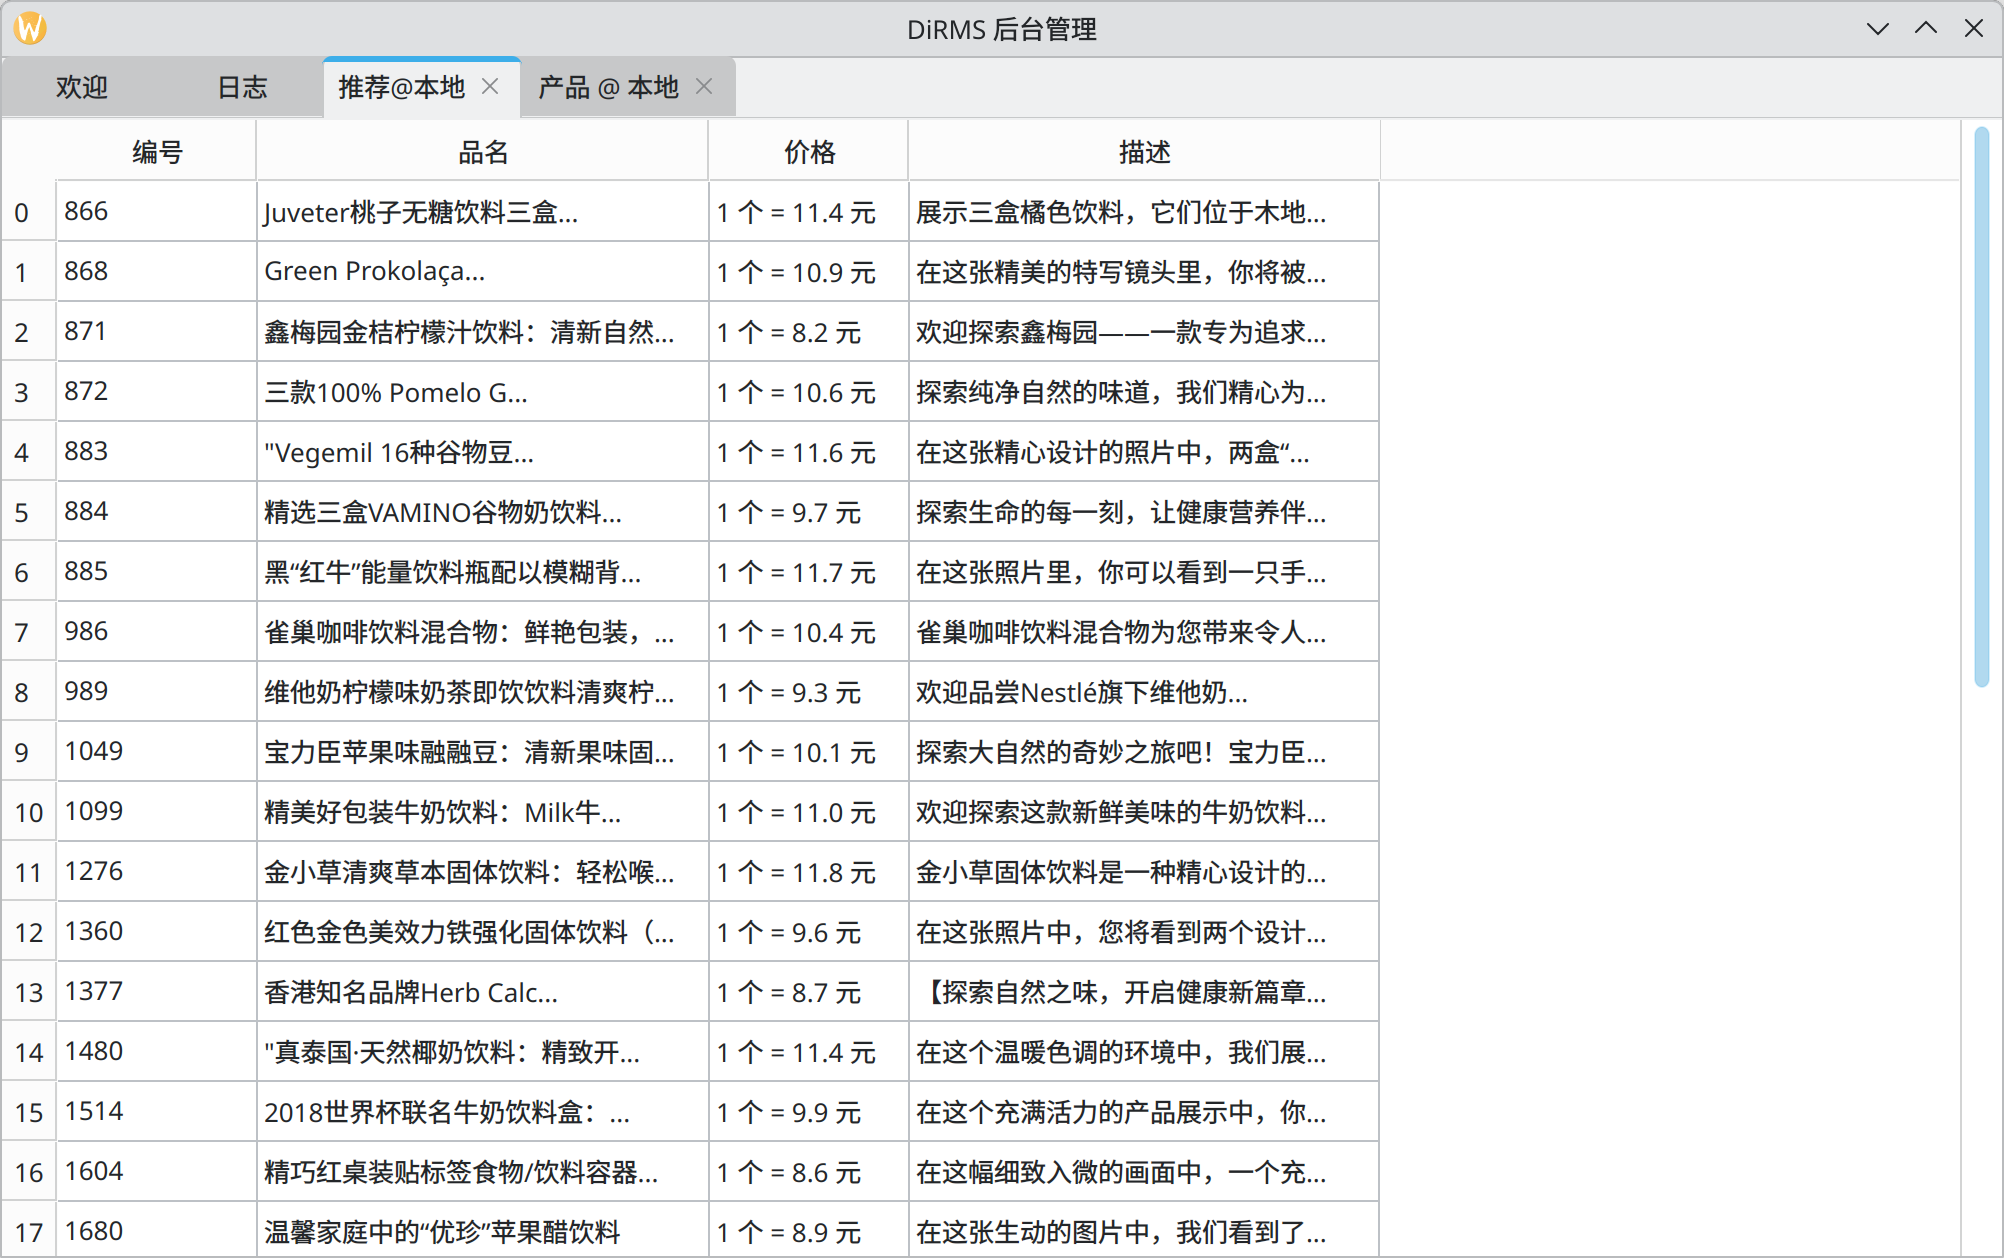
\includegraphics[width=0.8\textwidth]{./exp/rma-feat.png}
	\caption{RmAdmin运行效果:推荐商品管理}
	\label{fig:rma-feat}
\end{figure}

相似的,用户可以通过从主界面进入如图 \ref{fig:rma-feat} 所示的推荐商品管理界面,通过与进货界面相似的粘贴商品ID的方式用户可以管理向用户推荐(在用户移动应用程序首页展示)的商品。

\subsubsection{RmAnalysis}

\begin{figure}[htbp]
    \centering
    \subfloat{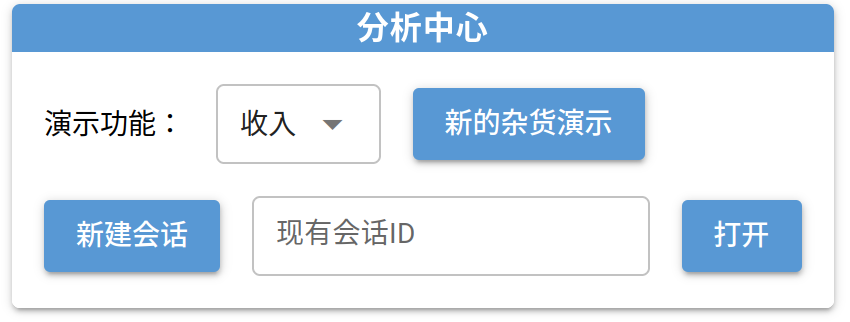
\includegraphics[width=0.5\textwidth]{./exp/aly-core-1.png}}
    \subfloat{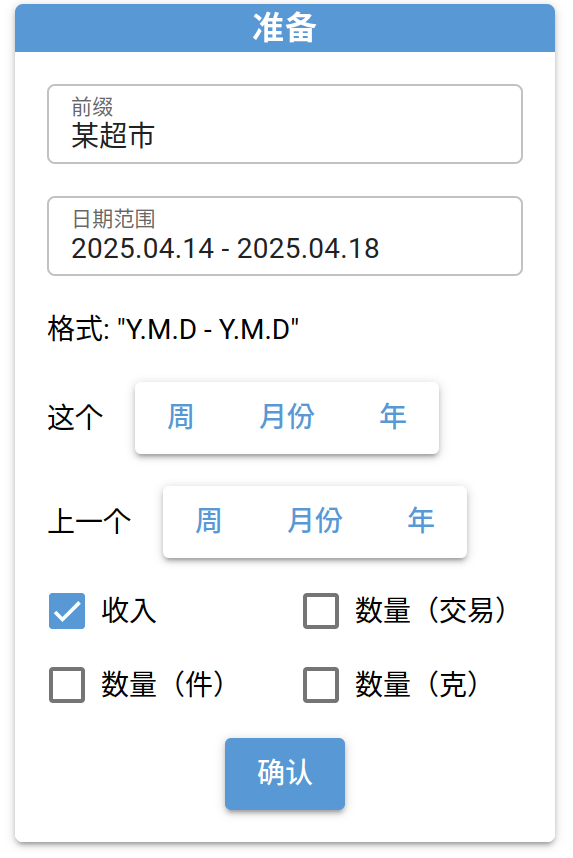
\includegraphics[width=0.3\textwidth]{./exp/aly-core-2.png}}
	\caption{RmAnalysis运行效果:基本界面}
	\label{fig:aly-core}
\end{figure}

通过前文提及RmGuard应用程序管理的RmAnalysis服务用于分析销售数据。通过访问服务的网页入口,用户可以访问到如图 \ref{fig:aly-core} 所示的分析主页、准备界面。用户可以利用会话ID(会话完成时间)打开先前保存的分析报告,也可以创建新的报告。在准备界面,用户可以自定义分析数据的时间范围(或者从画面中央的按钮快速选择),并制定需要分析的数值对象。以下为通过利用前文提及的超市销售数据数据集进行生成的图表和报告。

\begin{figure}[htbp]
    \centering
    \subfloat{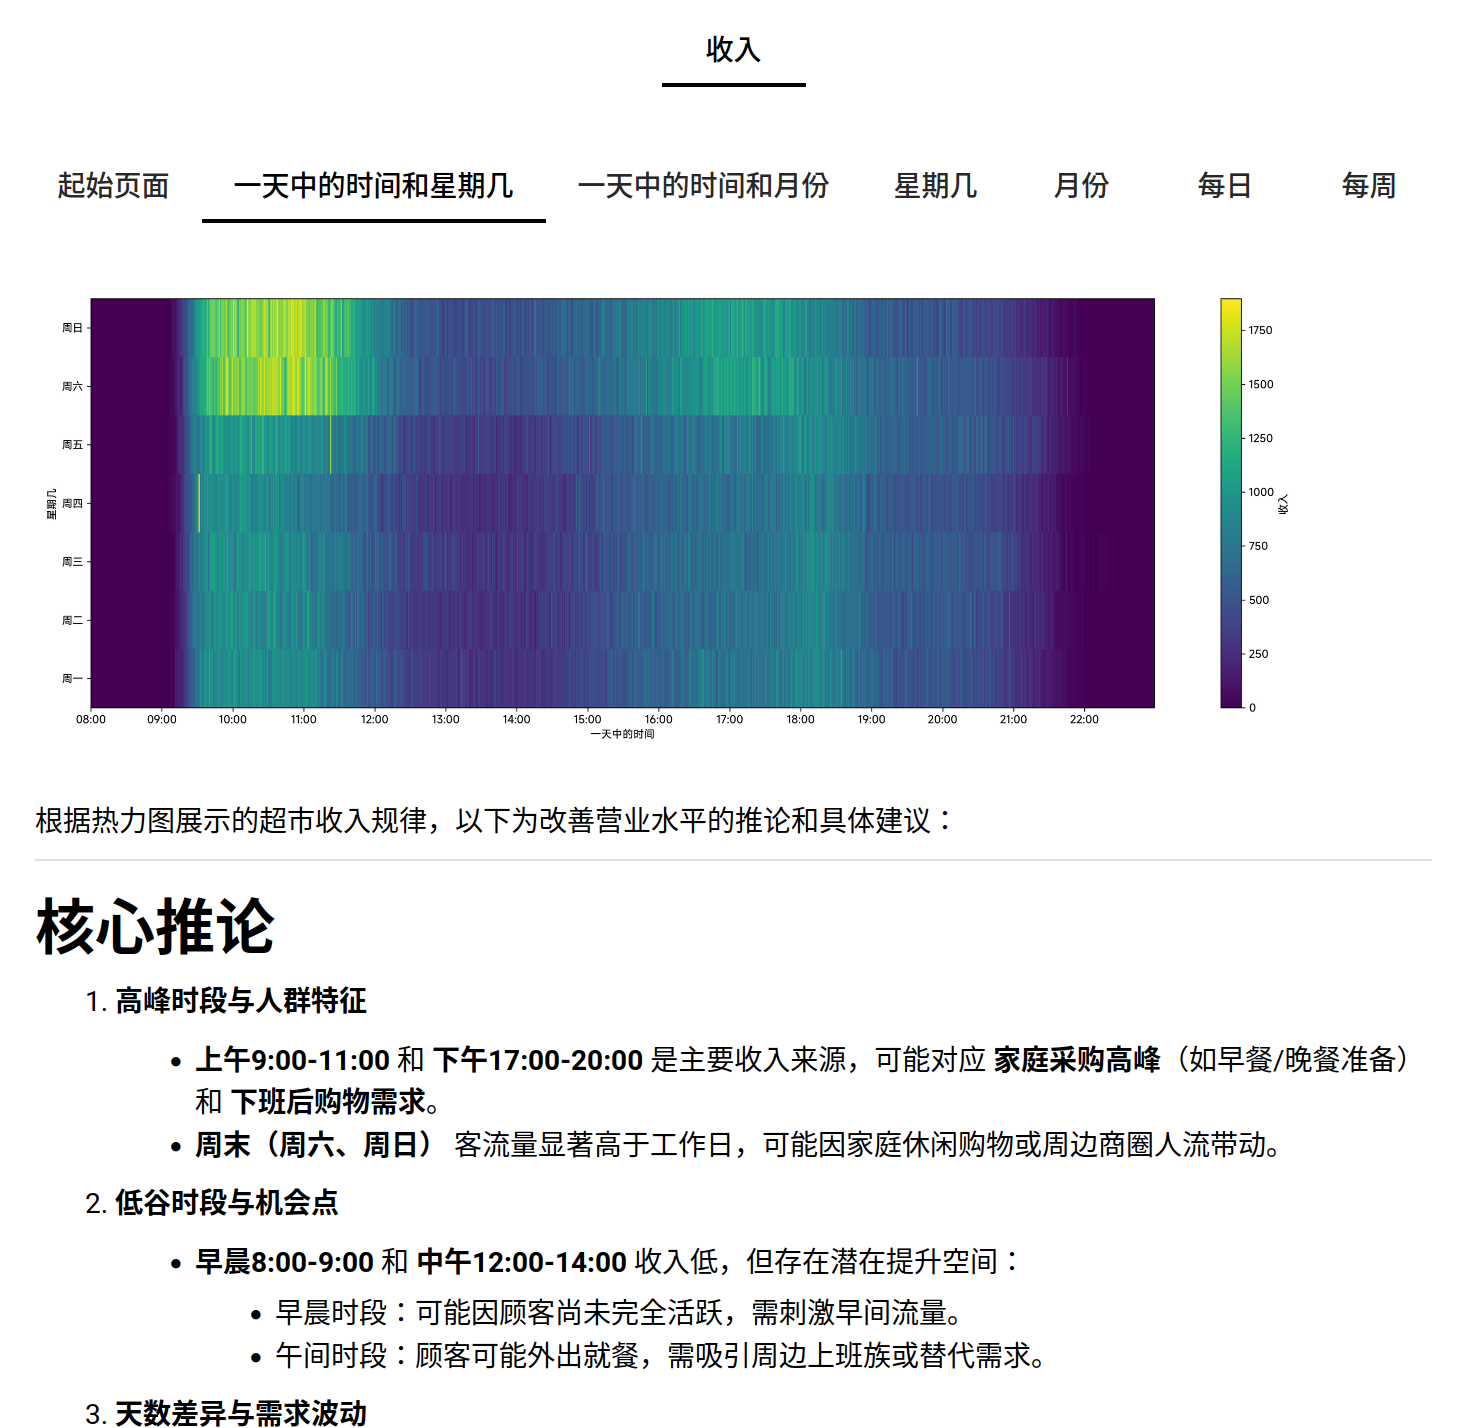
\includegraphics[width=0.4\textwidth]{./exp/aly-demo-1.png}}
    \subfloat{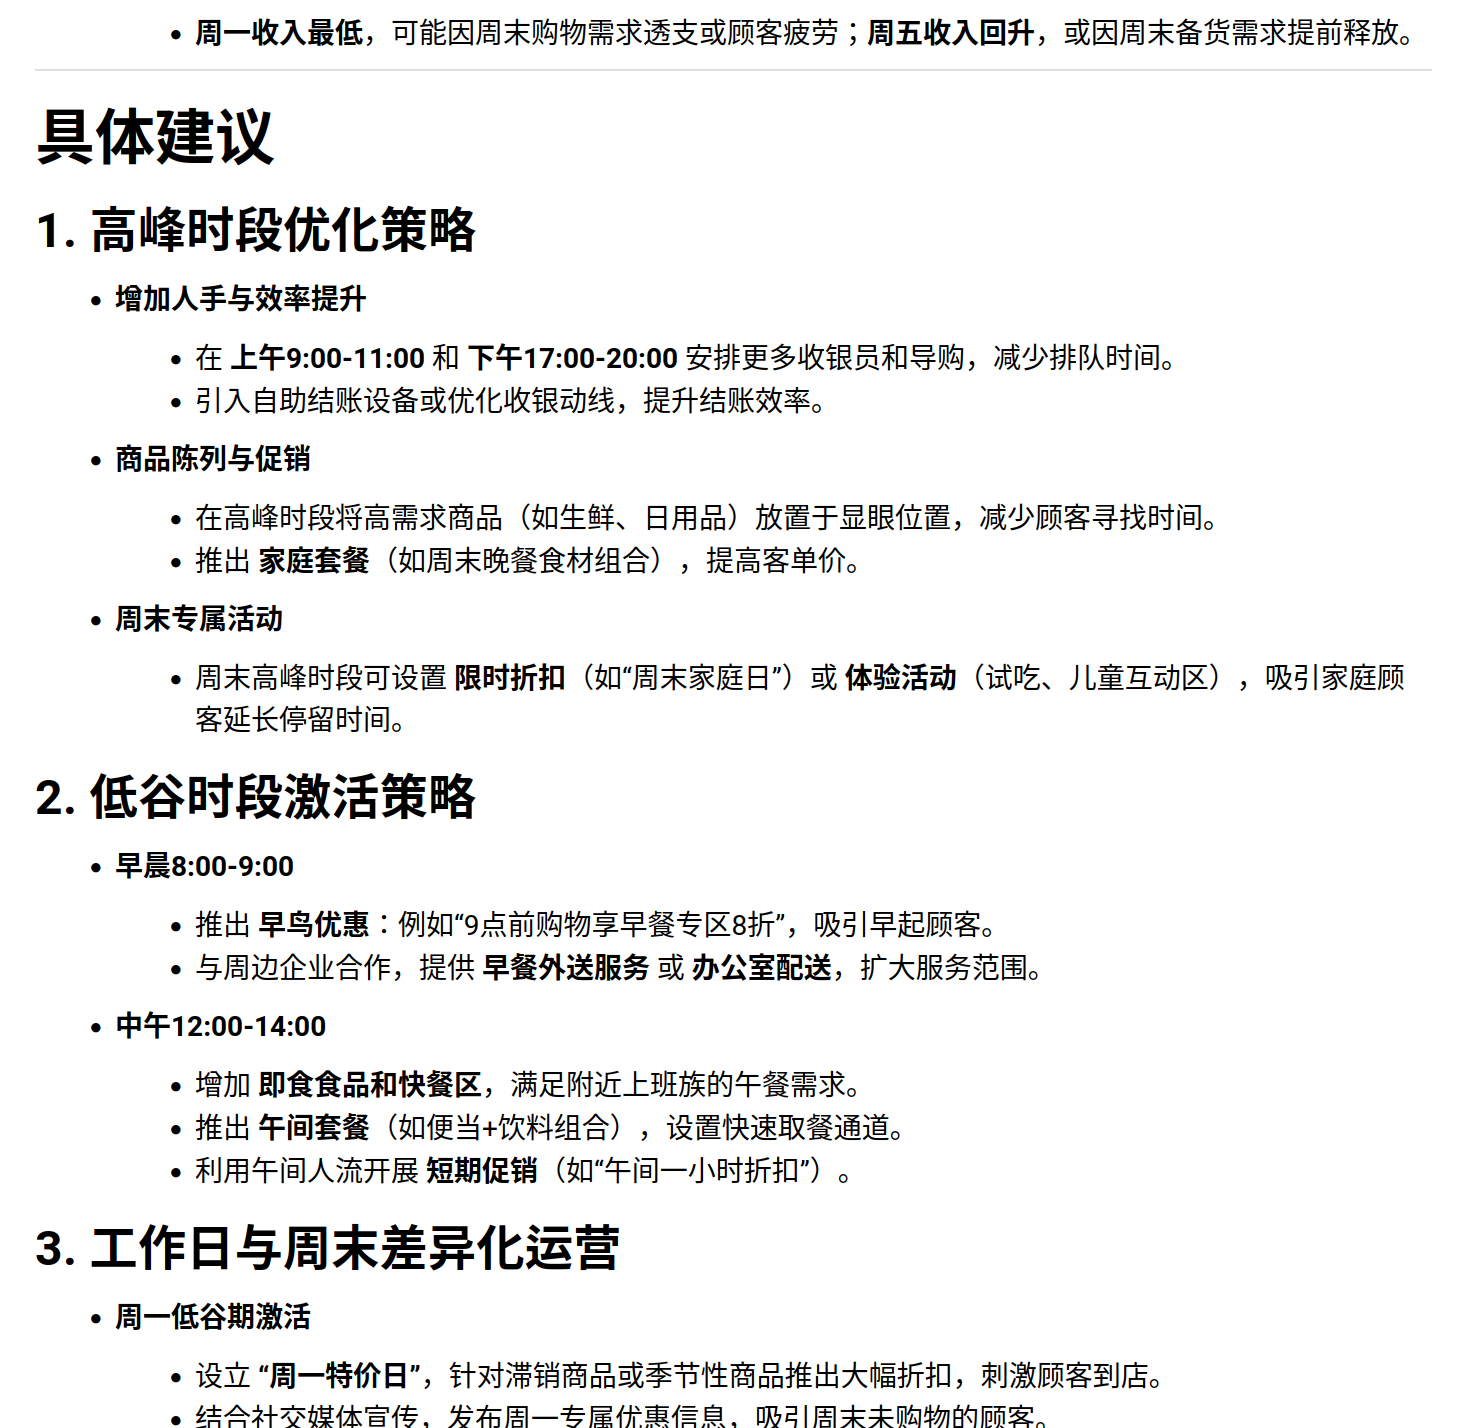
\includegraphics[width=0.4\textwidth]{./exp/aly-demo-2.png}}
	\caption{RmAnalysis运行效果:热力图分析}
	\label{fig:aly-demo-a}
\end{figure}

如图 \ref{fig:aly-demo-a} 所示,用户在热力图上可以通过观察该图表来获知营业收入(或者用户指定的任何其他变量)在一天中的变化规律($x$ 轴),同时可以在另一个轴看到利用另外一个(可以被天整除的,更长的)时间跨度(如周、月)上的规律变化。用户同时也可以从图表下侧的由AI生成的报告获得关于该图表的深入分析及与图表内容相关的营运建议以供参考。从AI给出的分析和报告上可知,在此AI顺利理解的该图表的基本要义并作出了较为精确的分析,并且提出了具体的、可以参考的建议。

\begin{figure}[htbp]
    \centering
    \subfloat{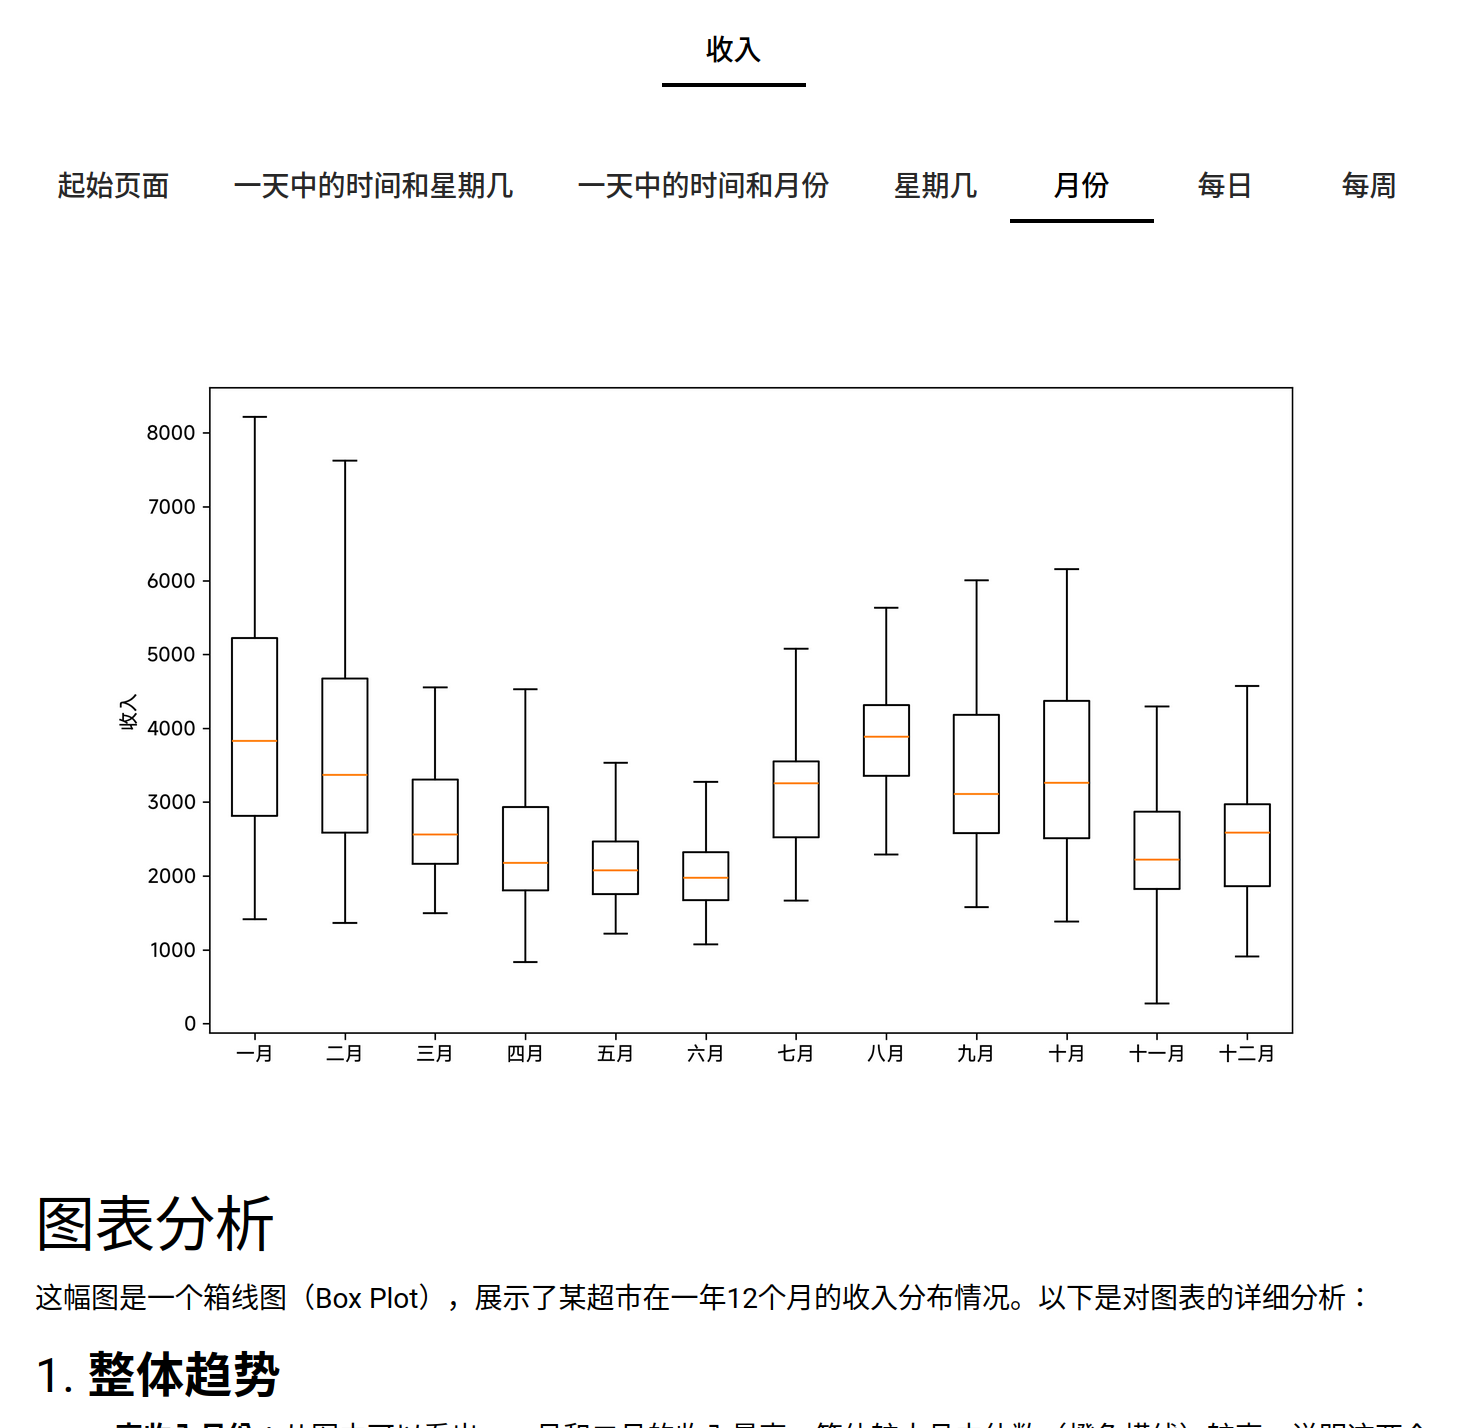
\includegraphics[width=0.4\textwidth]{./exp/aly-demo-3.png}}
    \subfloat{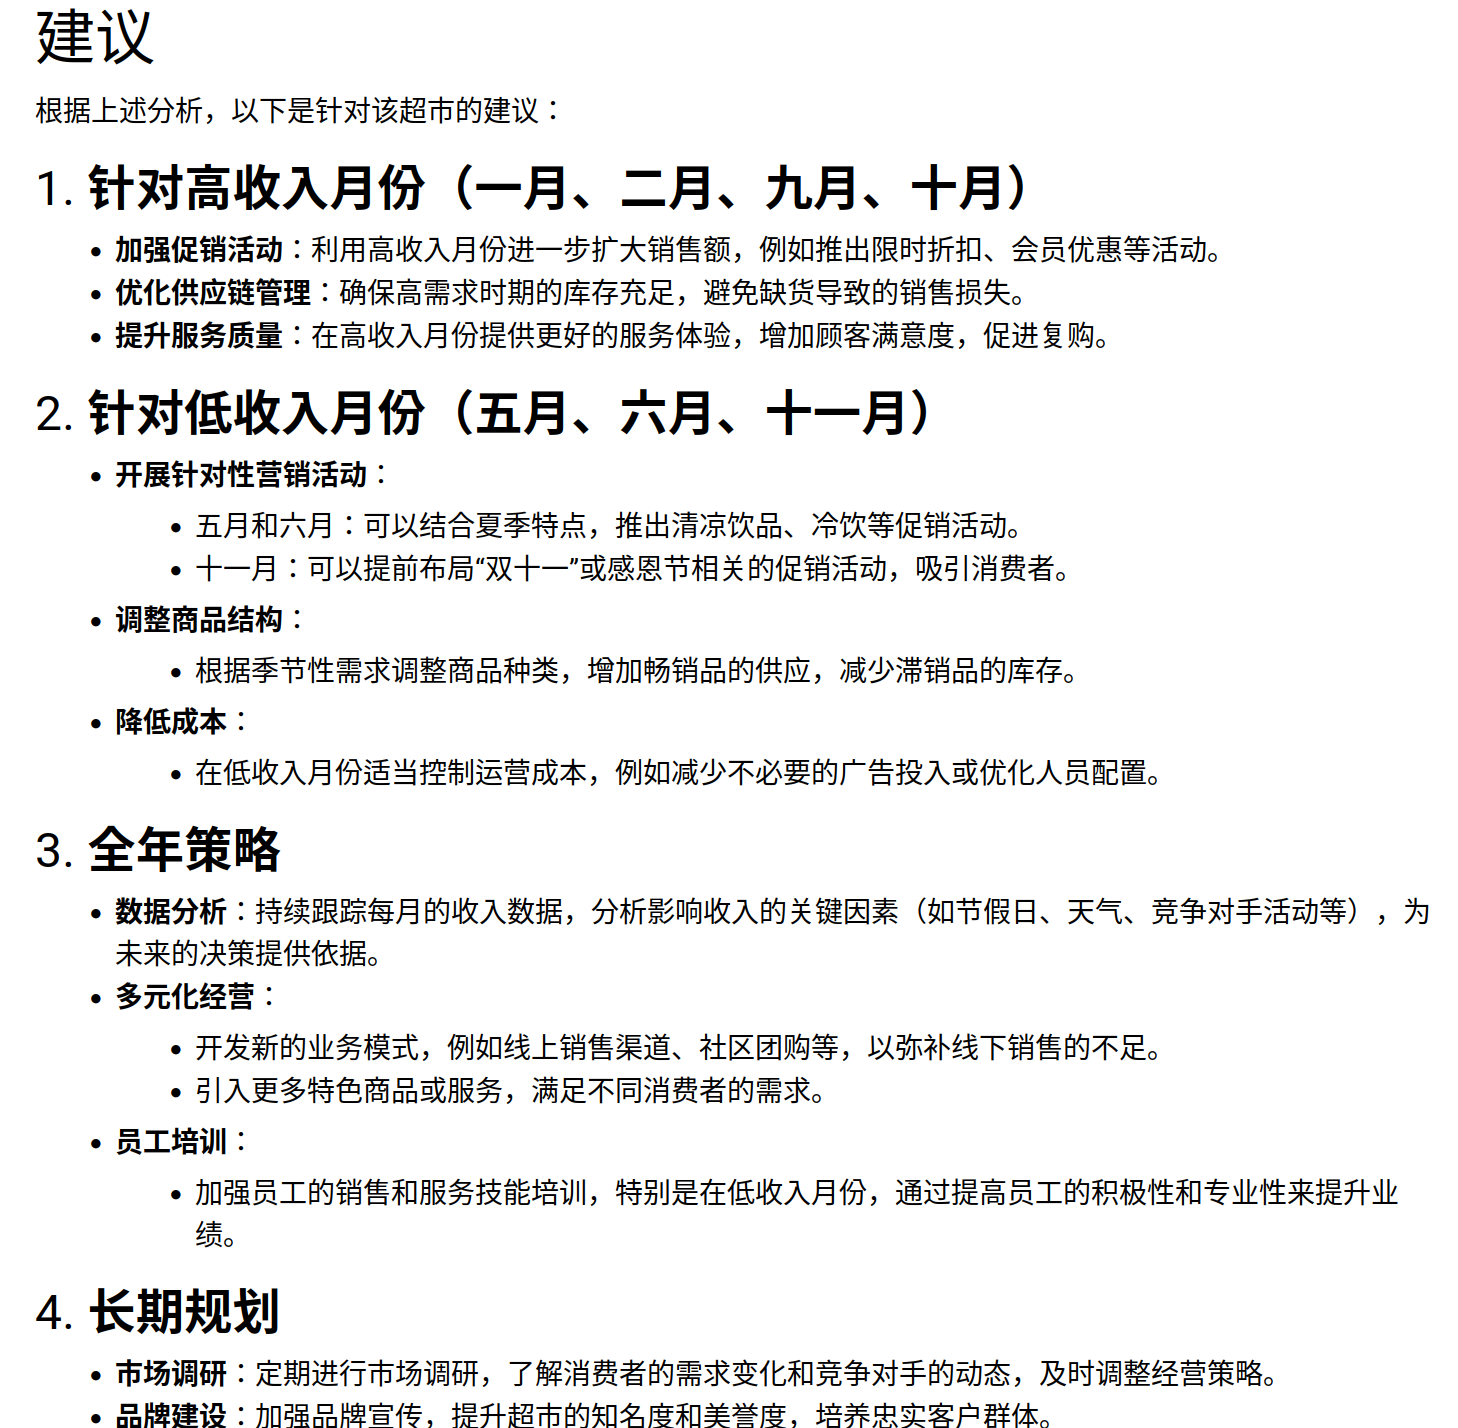
\includegraphics[width=0.4\textwidth]{./exp/aly-demo-4.png}}
	\caption{RmAnalysis运行效果:框图分析}
	\label{fig:aly-demo-b}
\end{figure}

\begin{figure}[htbp]
	\centering
	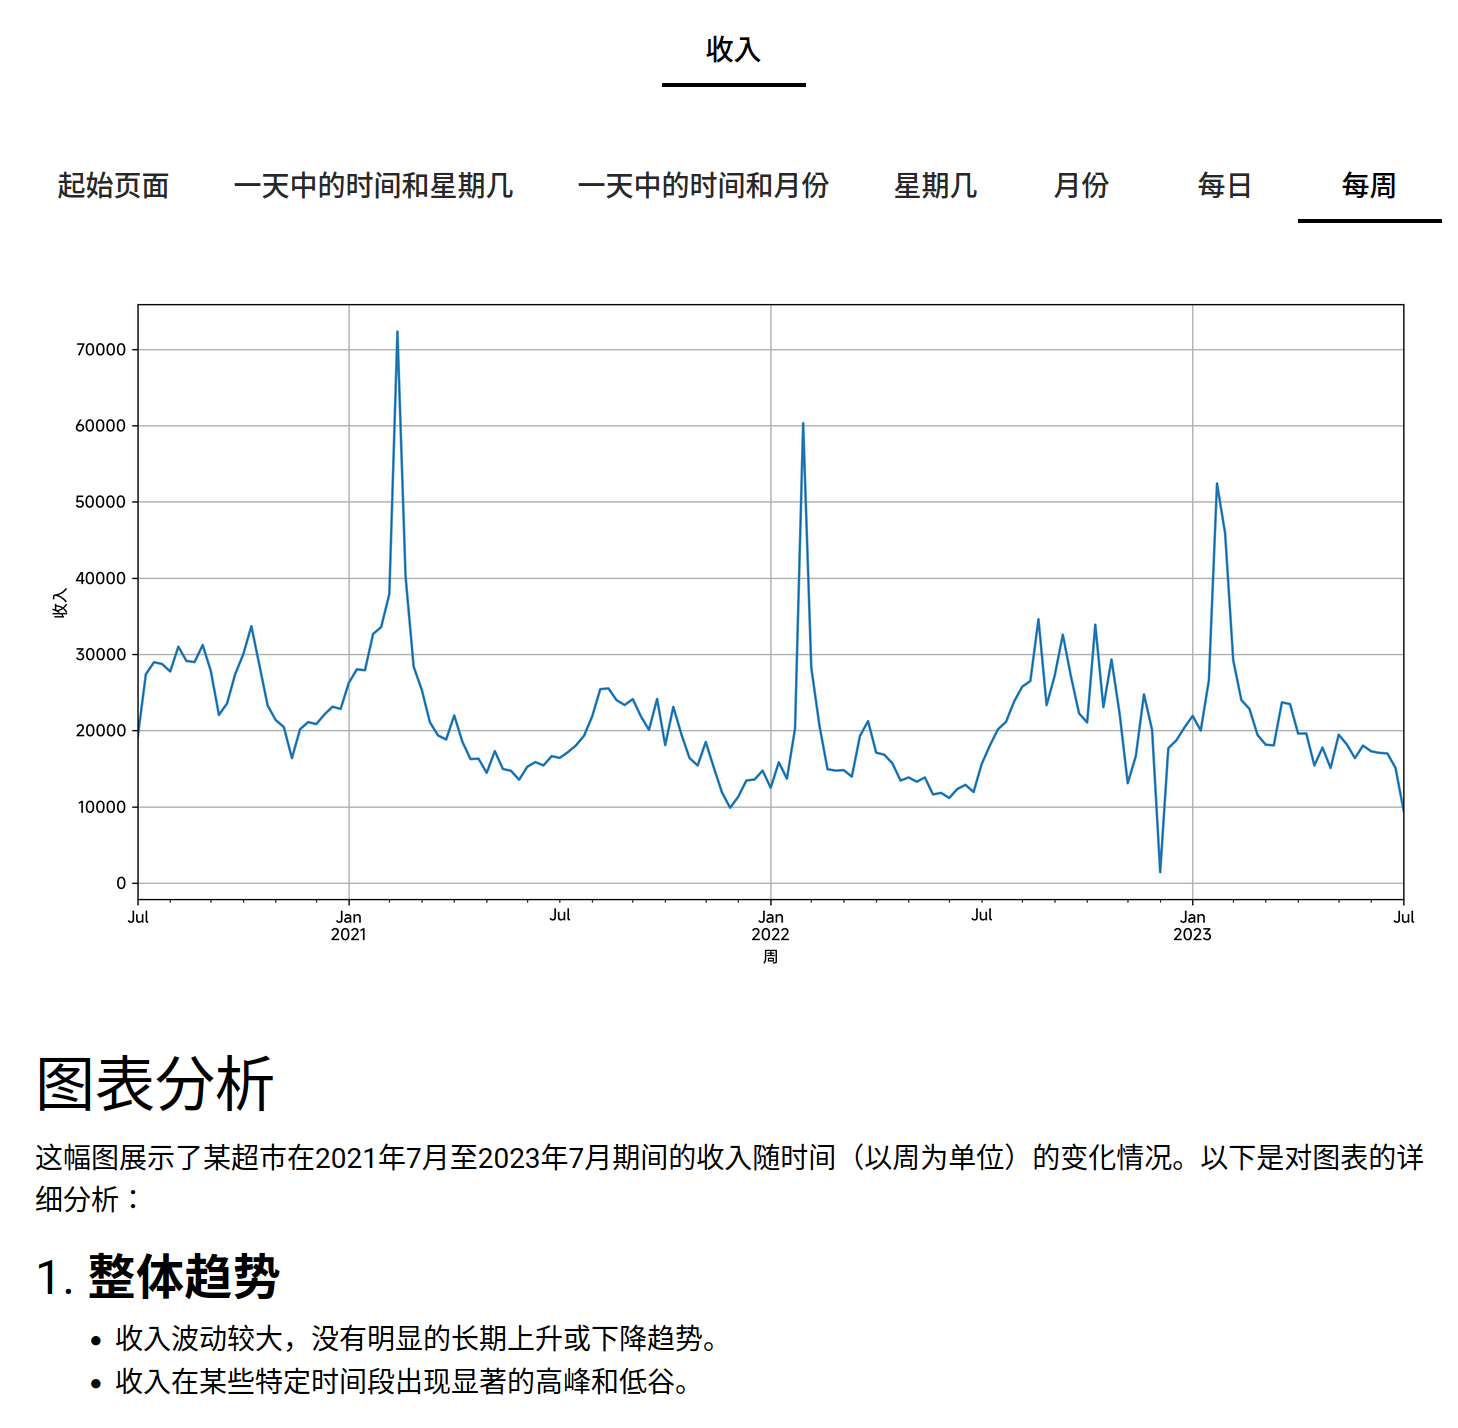
\includegraphics[width=0.5\textwidth]{./exp/aly-demo-5.png}
	\caption{RmAnalysis运行效果:折线图分析}
	\label{fig:aly-demo-5}
\end{figure}

如图 \ref{fig:aly-demo-b} 和 \ref{fig:aly-demo-5} 所示,用户在框图和折线图等其他类型的图表上也可以查看到其他的规律和统计,通过每个图表对于的AI总结用户也可以较为简单地获知从图表中可以看出的规律和相应的营运建议。

\subsubsection{ShopEyes Owner}

\begin{figure}[htbp]
    \centering
    \subfloat{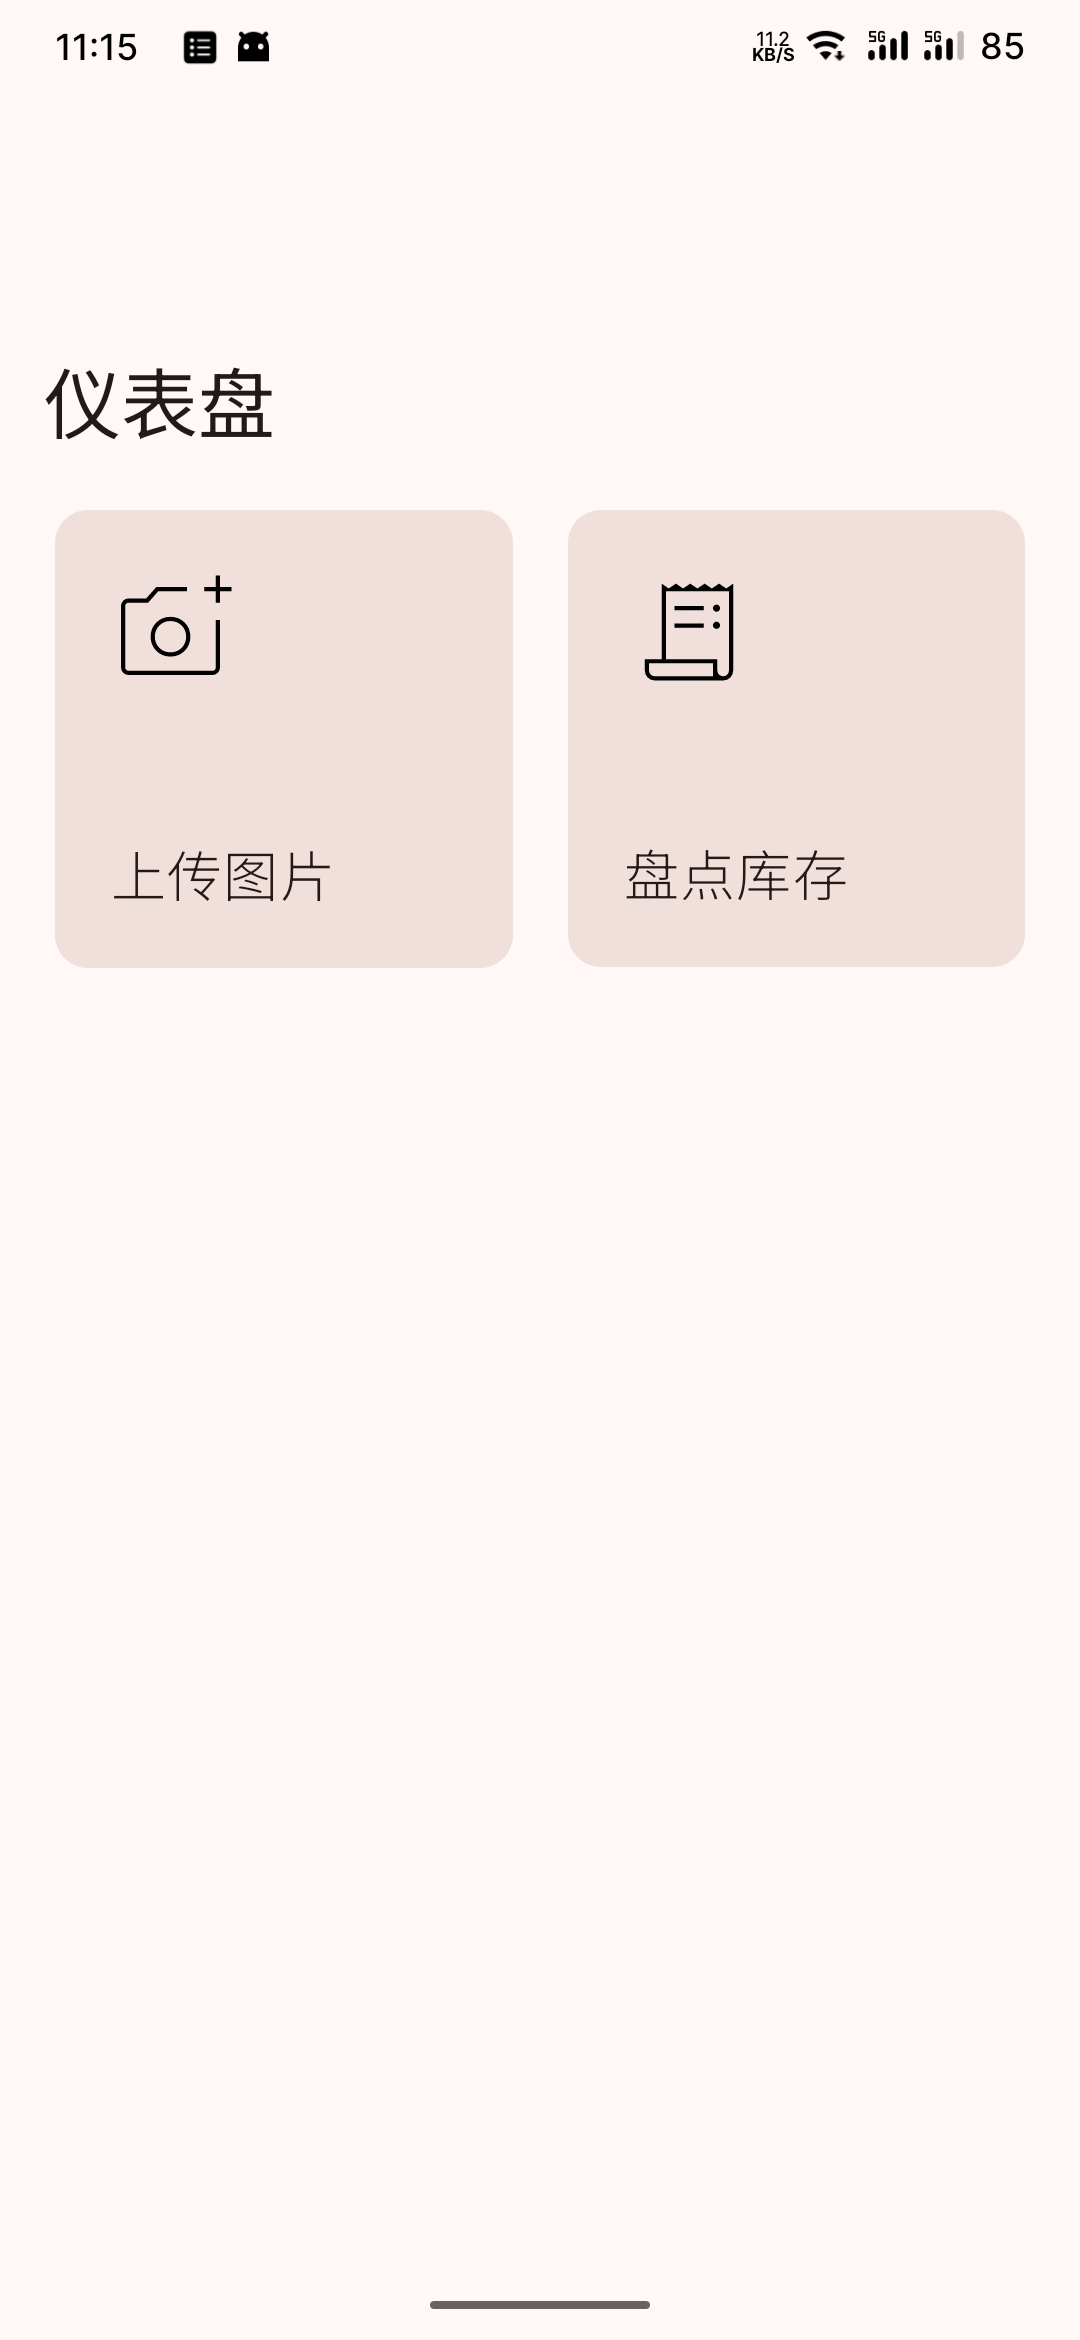
\includegraphics[width=0.2475\textwidth]{./exp/seo.png}}
    \hfill
    \subfloat{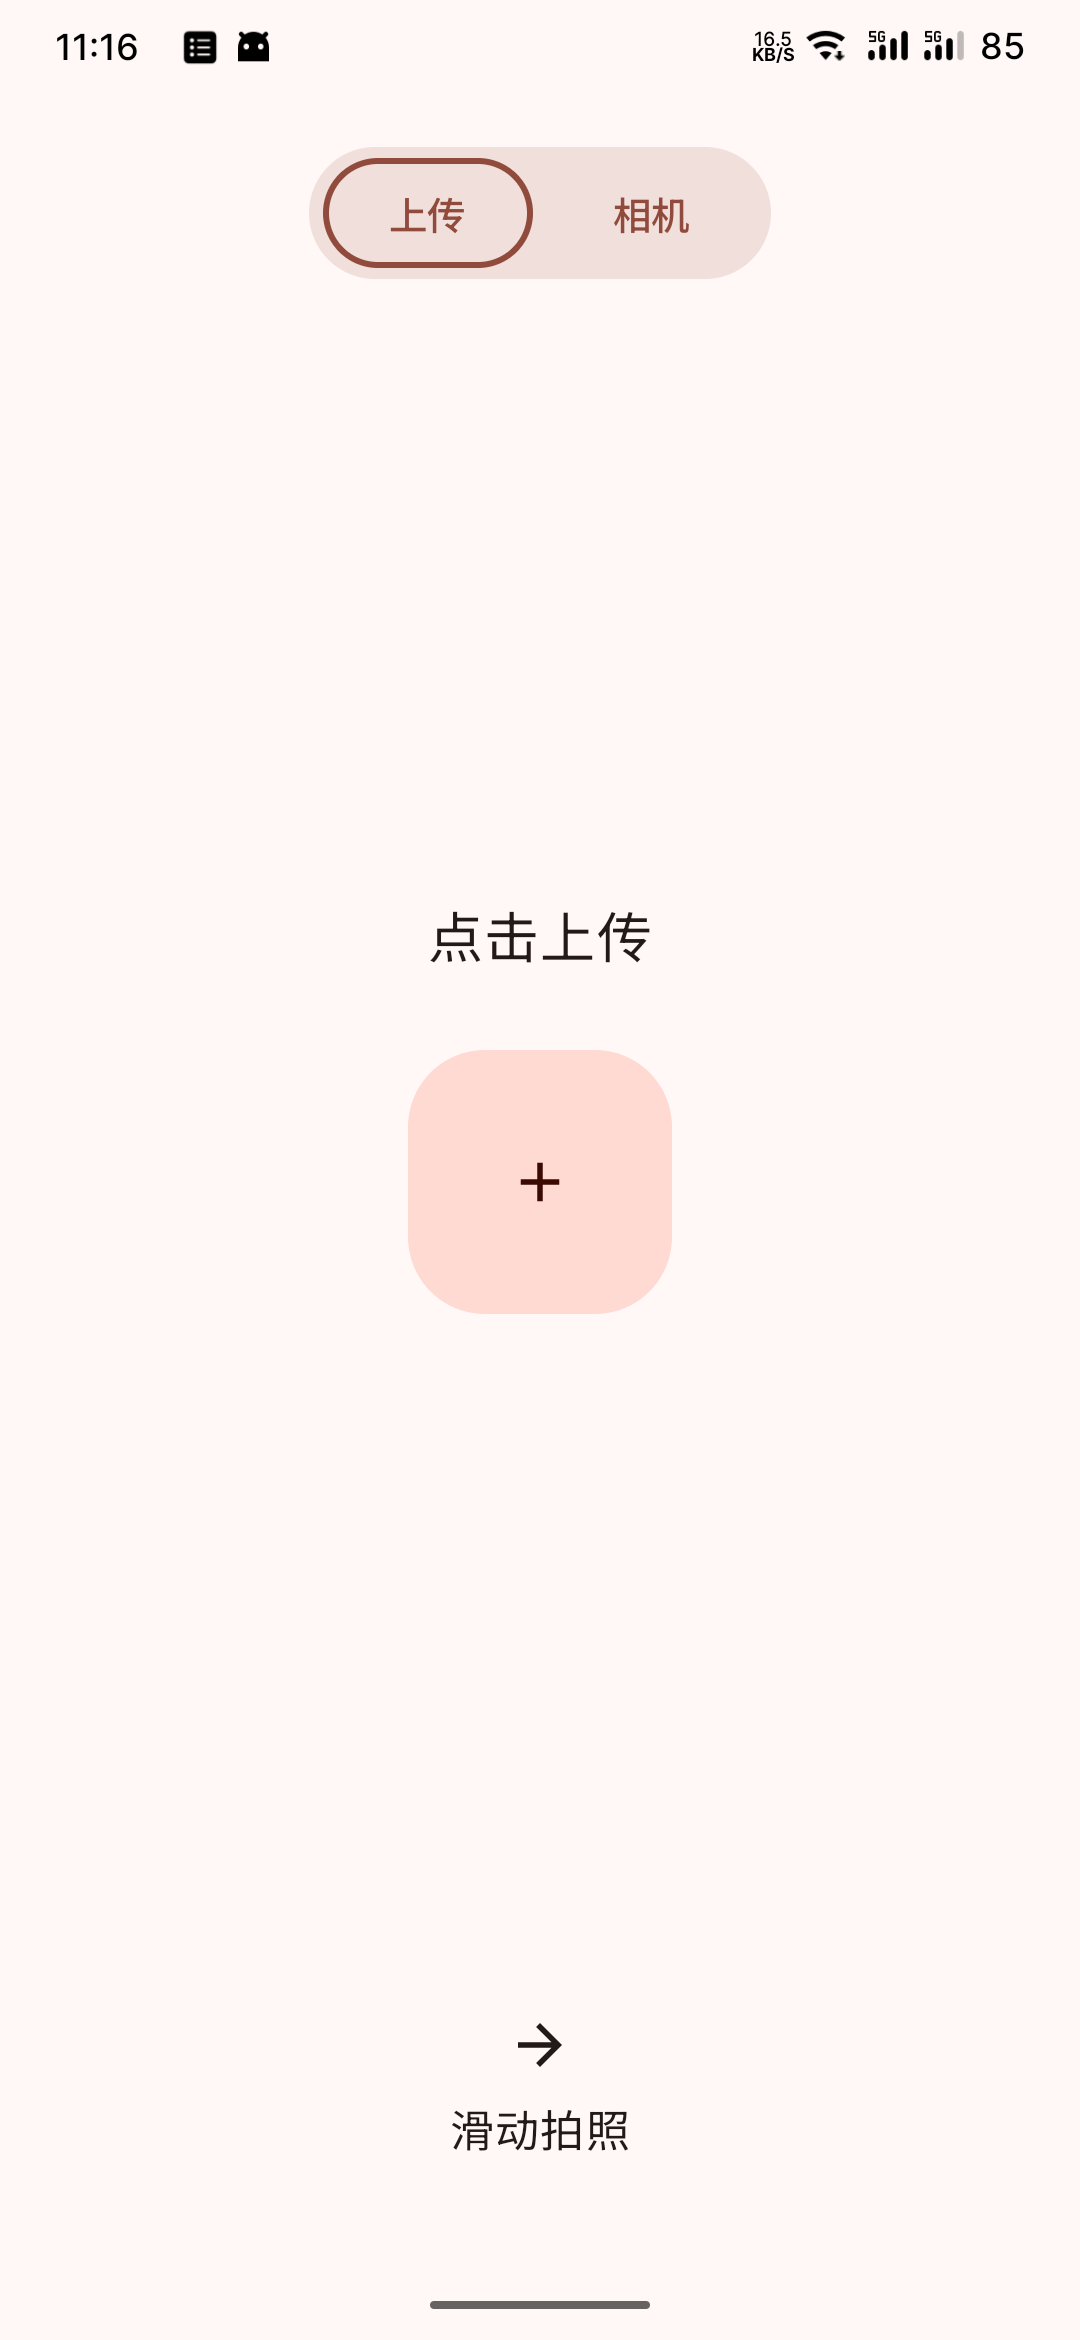
\includegraphics[width=0.2475\textwidth]{./exp/seo-local.png}}
    \hfill
    \subfloat{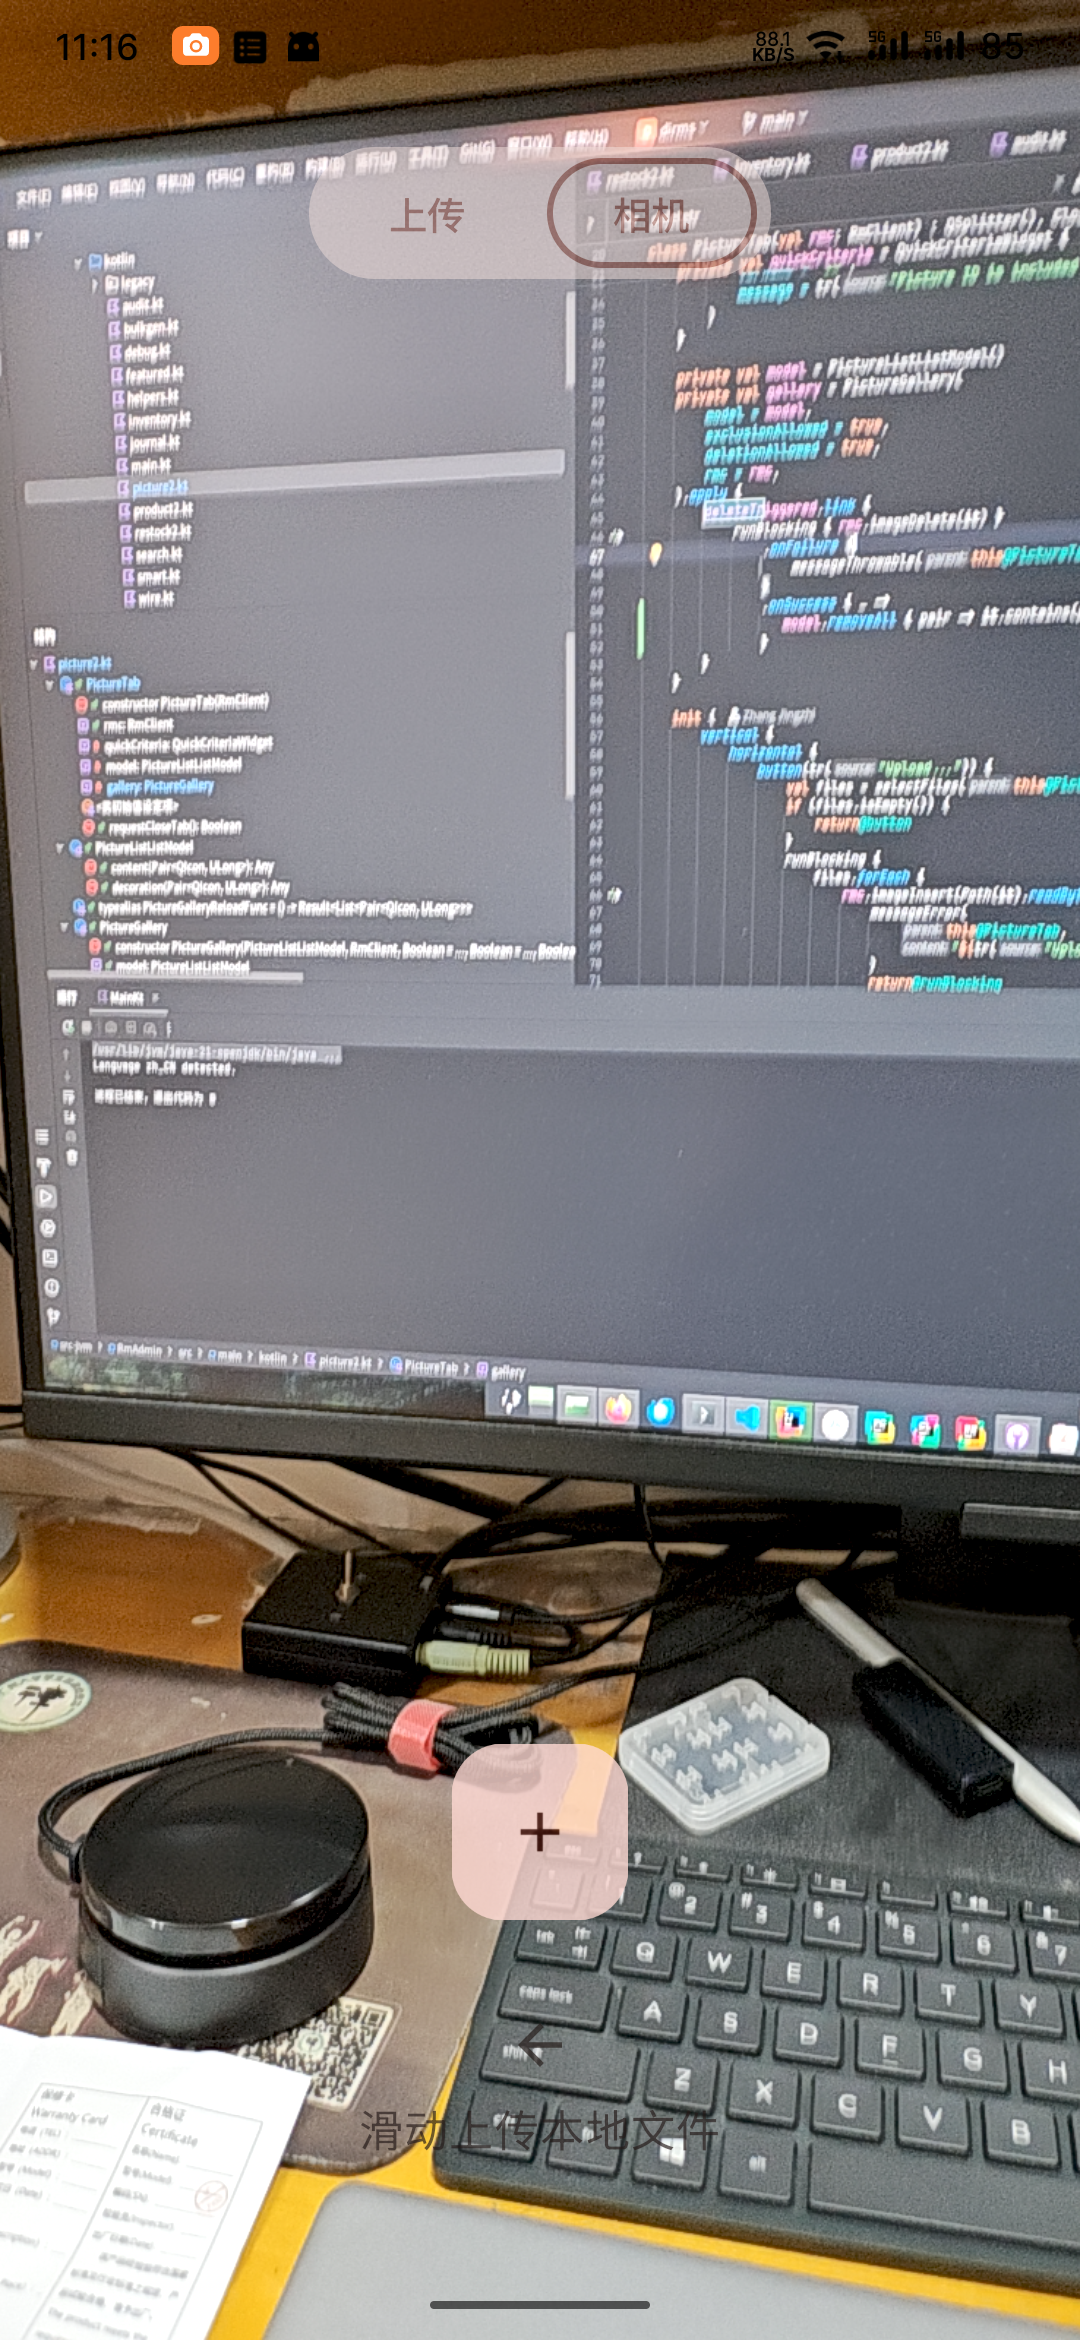
\includegraphics[width=0.2475\textwidth]{./exp/seo-camera.png}}
    \hfill
    \subfloat{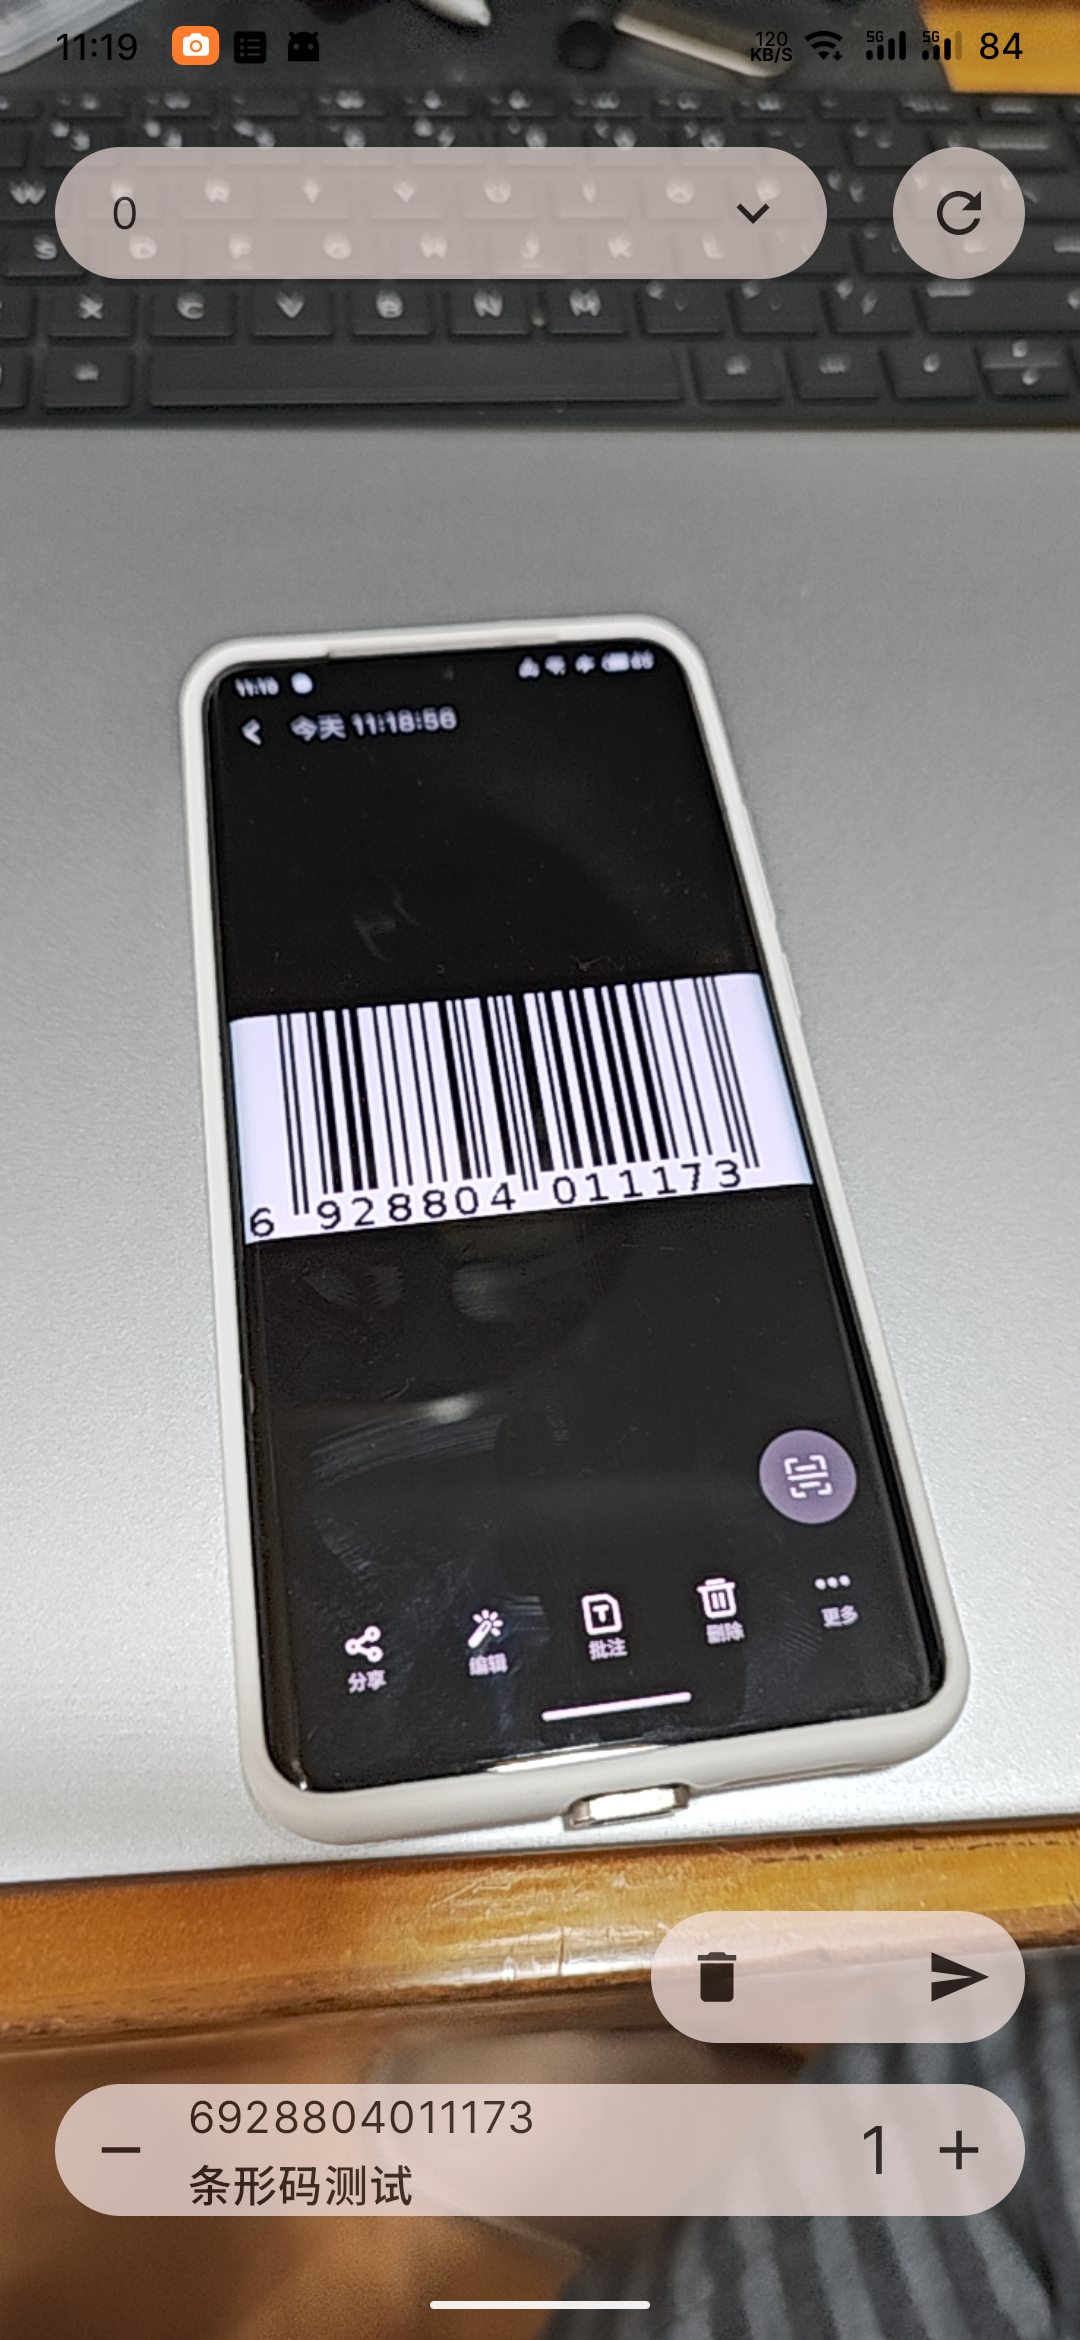
\includegraphics[width=0.2475\textwidth]{./exp/seo-audit.png}}
	\caption{ShopEyes运行效果}
	\label{fig:seo}
\end{figure}

如图 \ref{fig:seo} 所示,ShopEyes应用程序的商家(Owner)端提供了在移动设备上上传本地图片或拍照的功能。在上传本地图片的界面上,用户通过点击画面中心的按钮将唤出设备自带的图片选择界面,用户可以选择手机相册中预先准备的照片;在拍摄界面上,用户通过点击按钮可以将取景器中的画面保存为照片并上传。通过滑动或点击上方标签,用户可以更改图片来源类型。

同时,用户可以利用AI条码识别功能进行点货,用户可以在点货界面(最右图)画面顶部选择点货批次。而在画面中条形码被识别之后,画面底部将会列出条形码及其所对应的商品名称。用户可以通过点击每项左侧和右侧的按钮来调整货品数量。通过点击项目列表上侧胶囊型按钮的左侧,可以清除目前记录的待提交条目,而通过点击右侧按钮可以提交当前积压的条目。

\subsubsection{EasyDataset}

\begin{figure}[htbp]
    \centering
    \subfloat{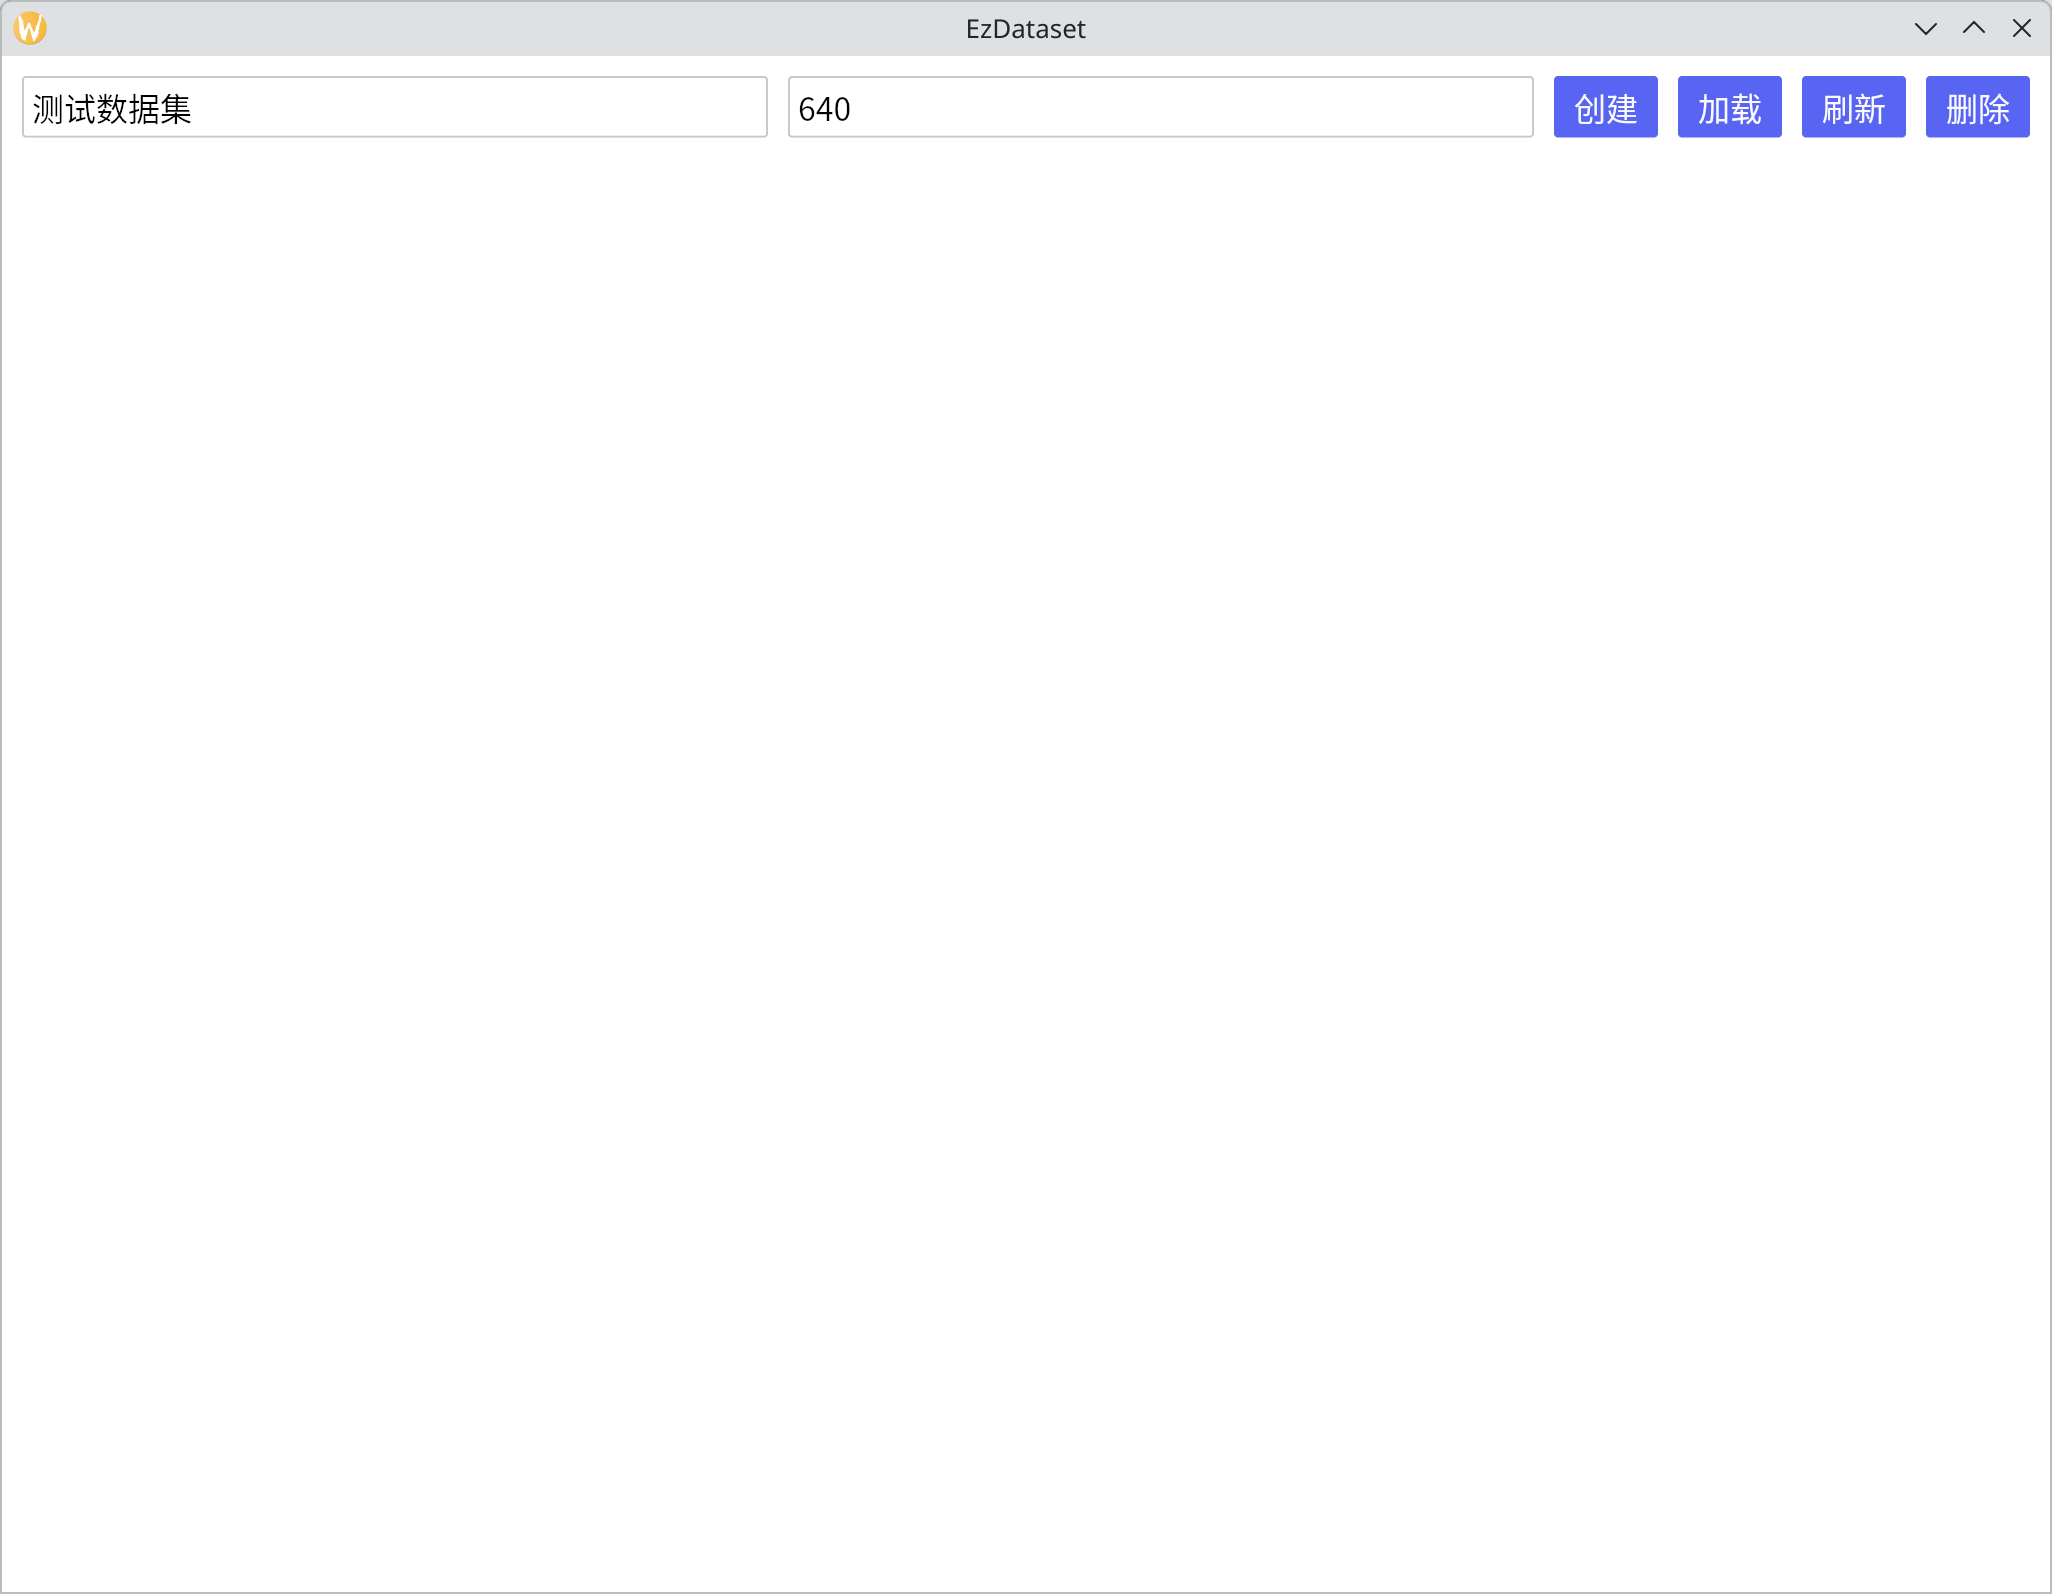
\includegraphics[width=0.45\textwidth]{./exp/ed-nd-1.png}}
    \hfill
    \subfloat{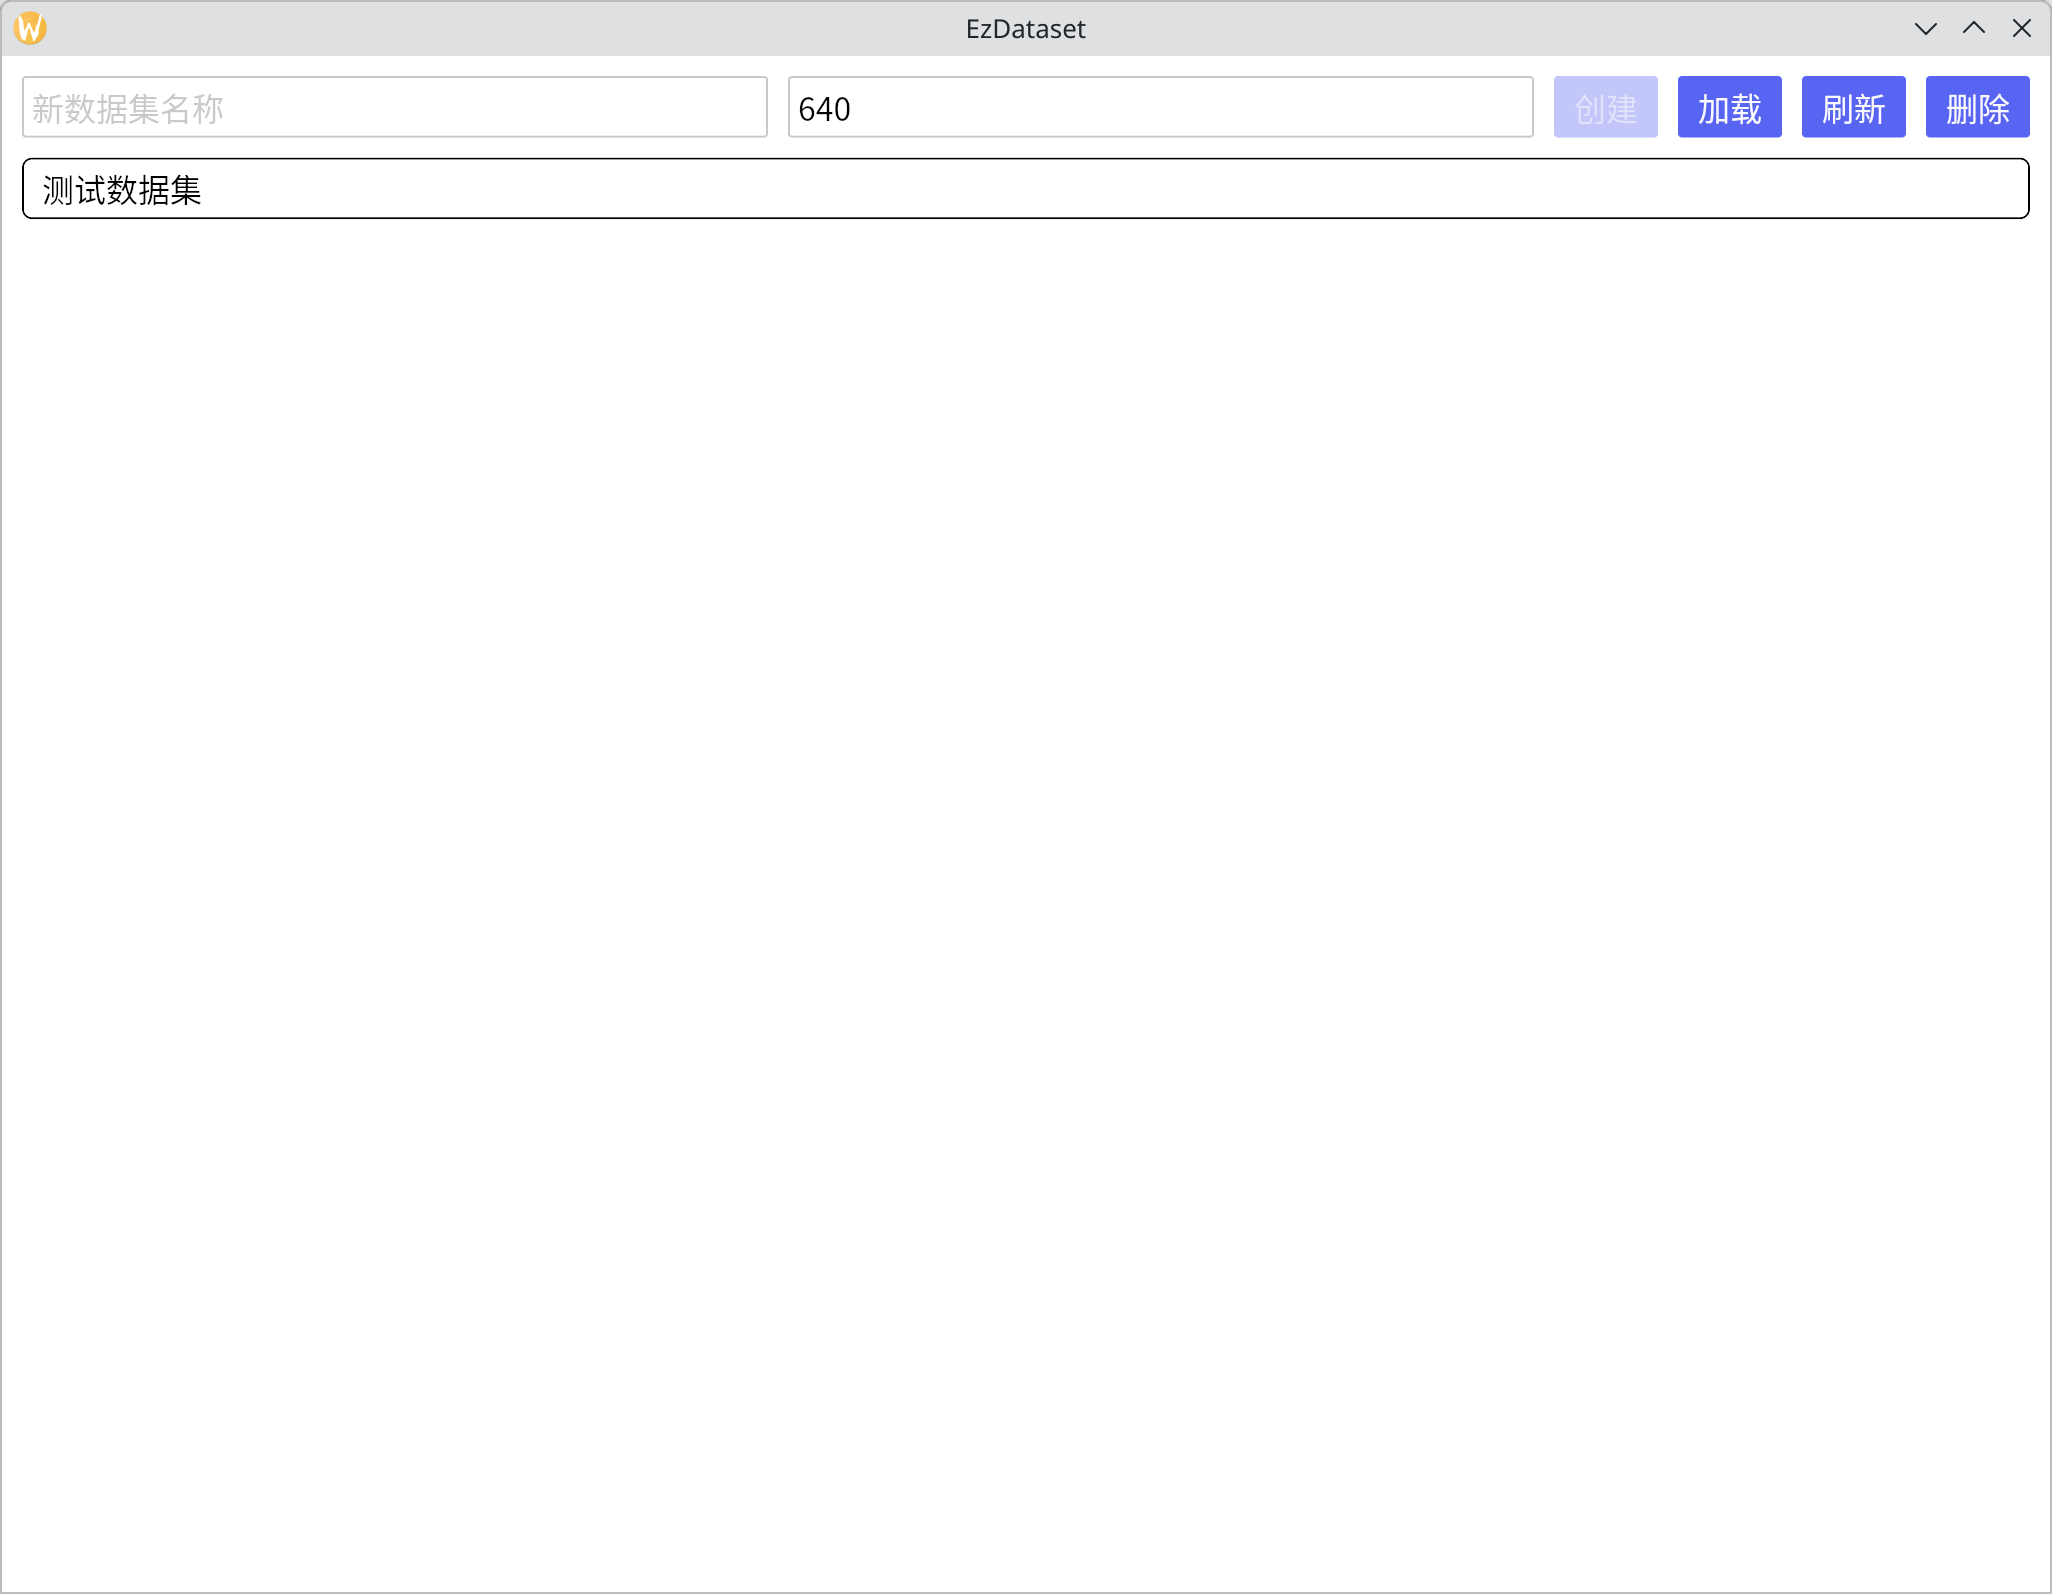
\includegraphics[width=0.45\textwidth]{./exp/ed-nd-2.png}}
	\caption{EasyDataset运行效果:数据集管理}
	\label{fig:ed-nd}
\end{figure}

EasyDataset是用于创建训练商品识别用数据集的应用程序。如图 \ref{fig:ed-nd} 所示,用户可以指定数据集的名字和图像边长,点击“创建”按钮来创建数据集,在列表中选择数据集后通过点击“加载”按钮可以打开之。

\begin{figure}[htbp]
    \centering
    \subfloat{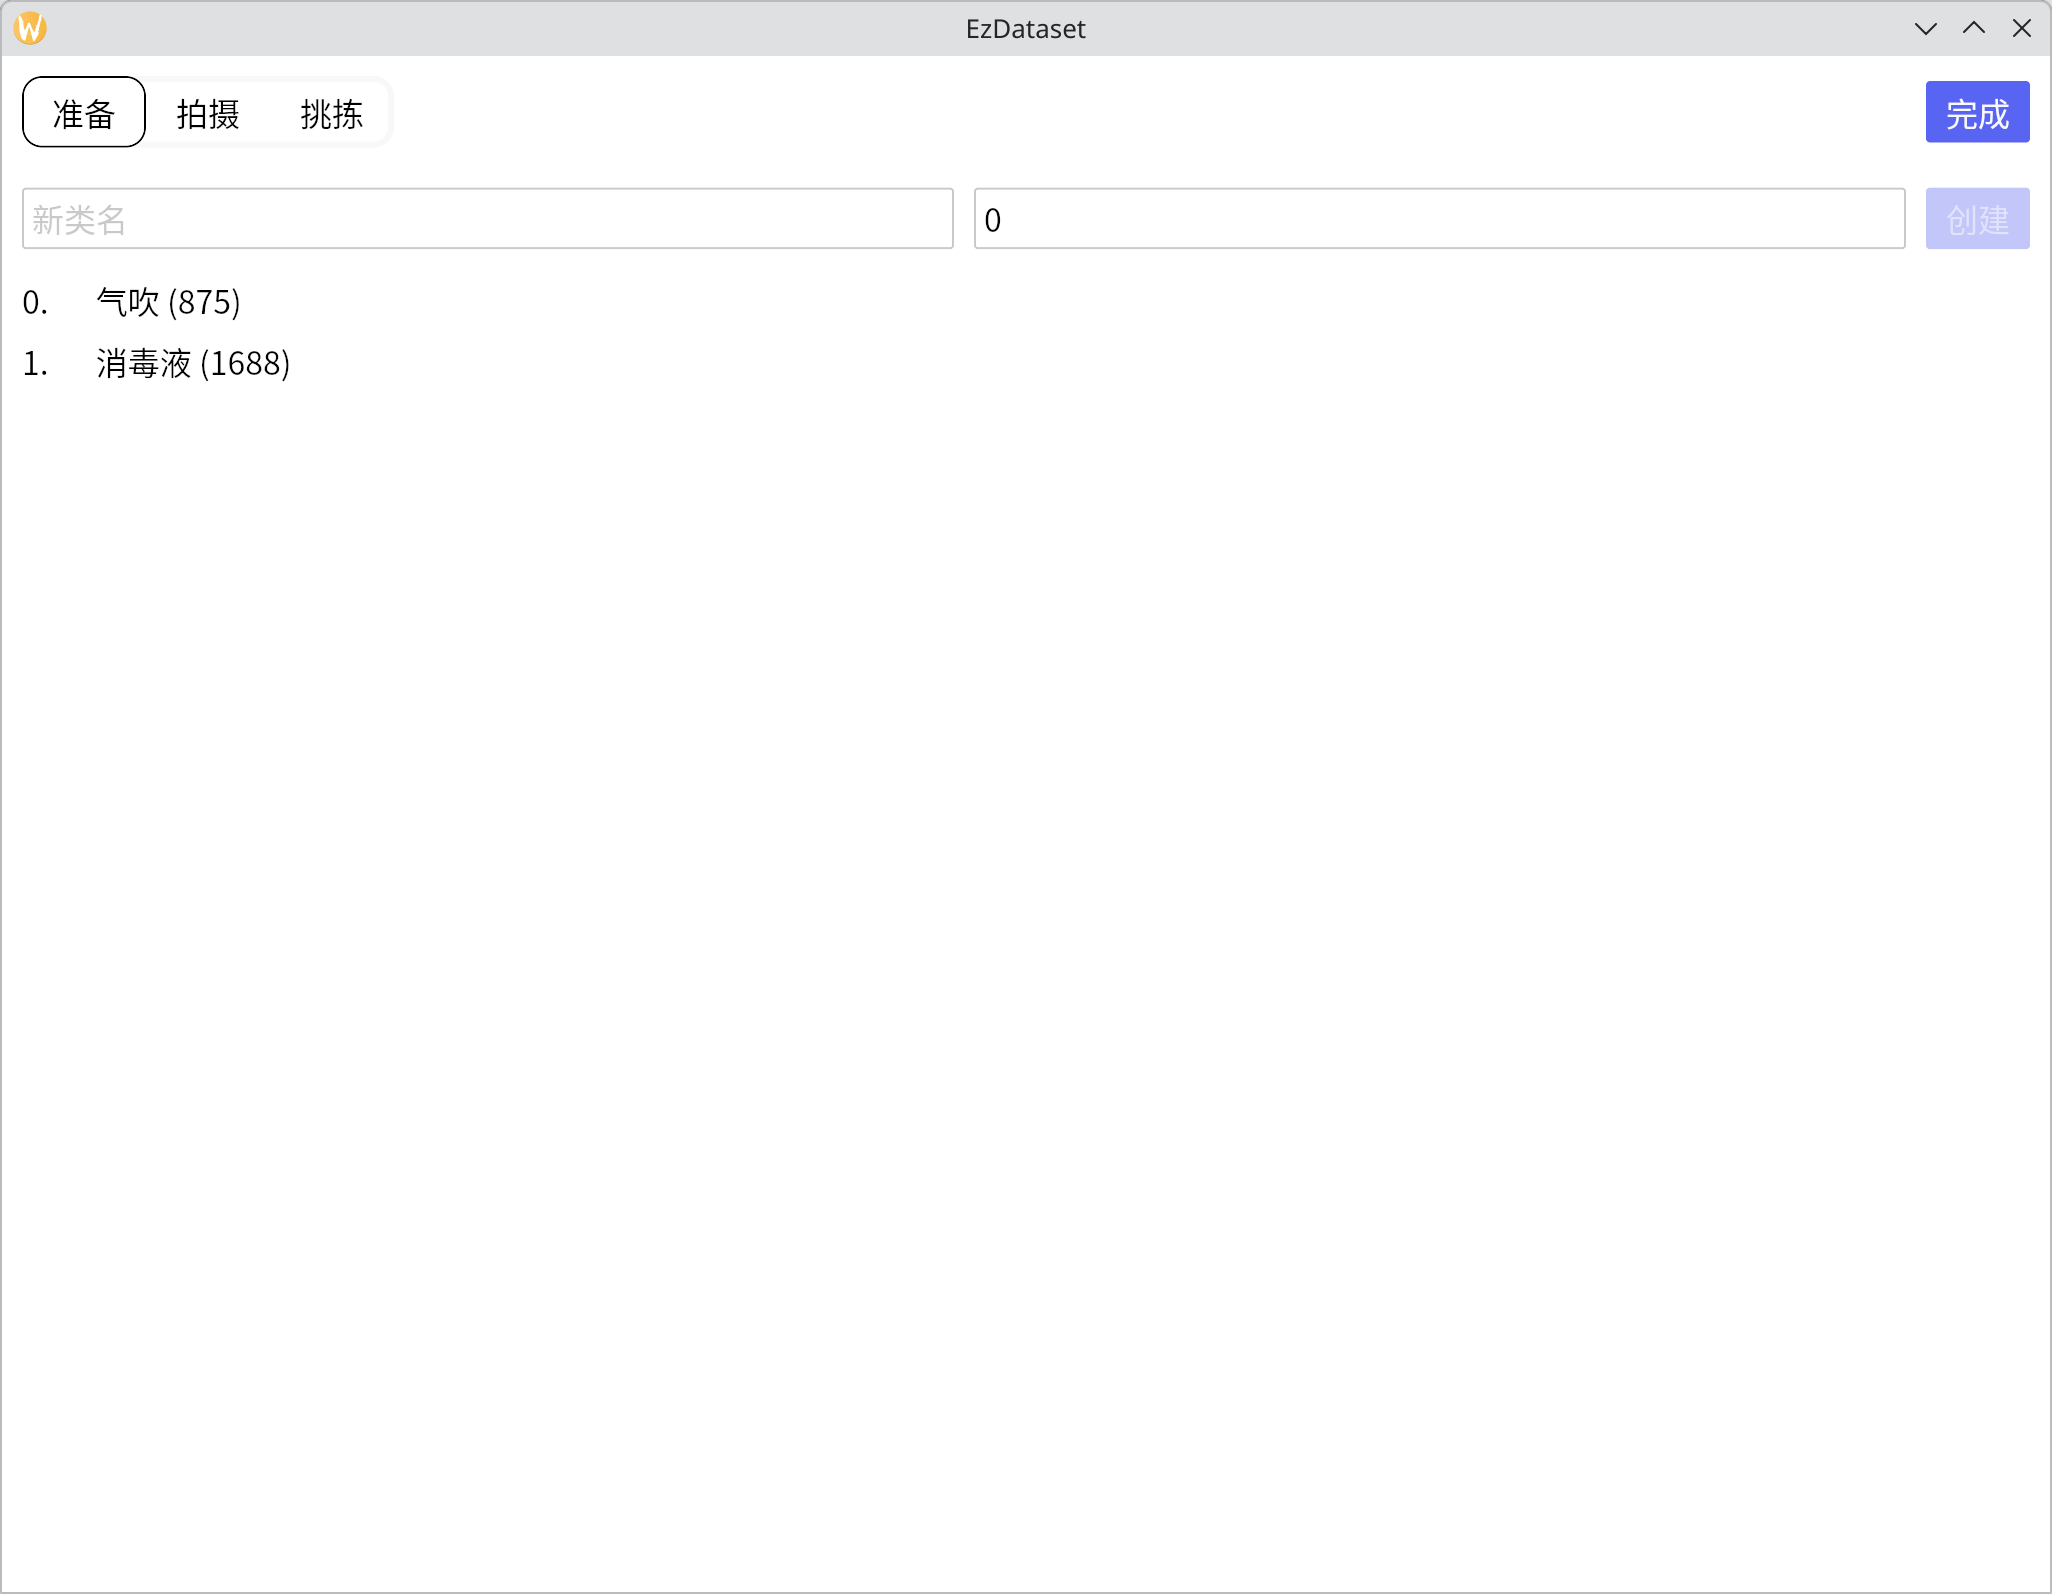
\includegraphics[width=0.33\textwidth]{./exp/ed-nc.png}}
    \hfill
    \subfloat{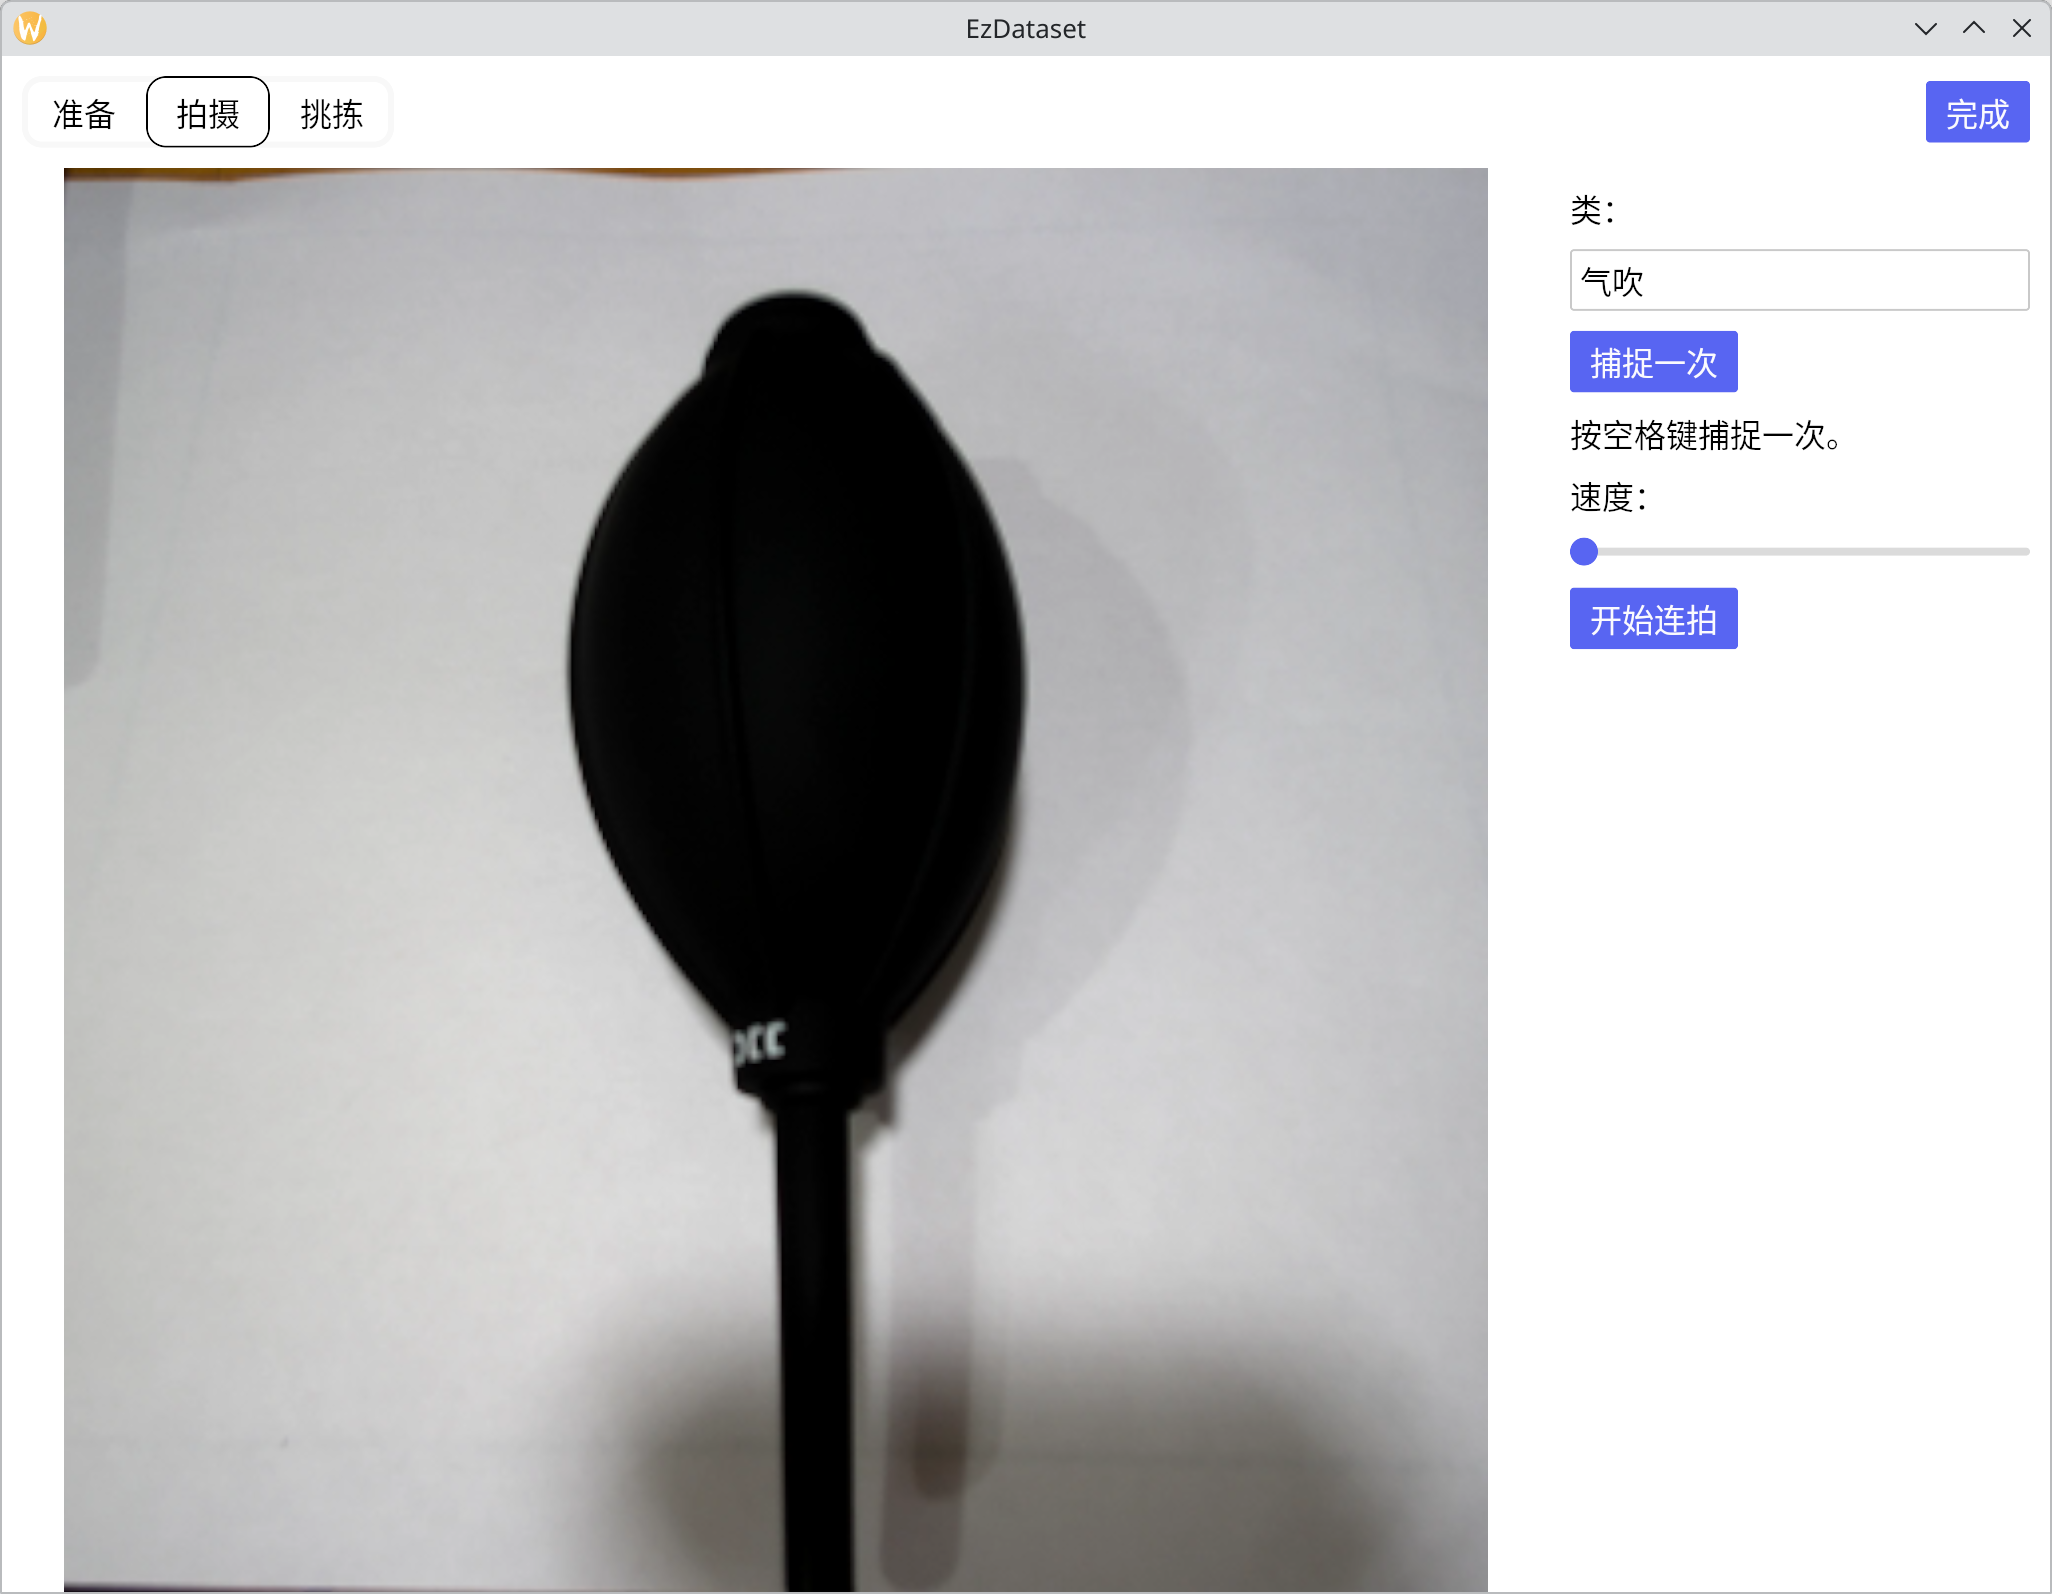
\includegraphics[width=0.33\textwidth]{./exp/ed-shot.png}}
    \hfill
    \subfloat{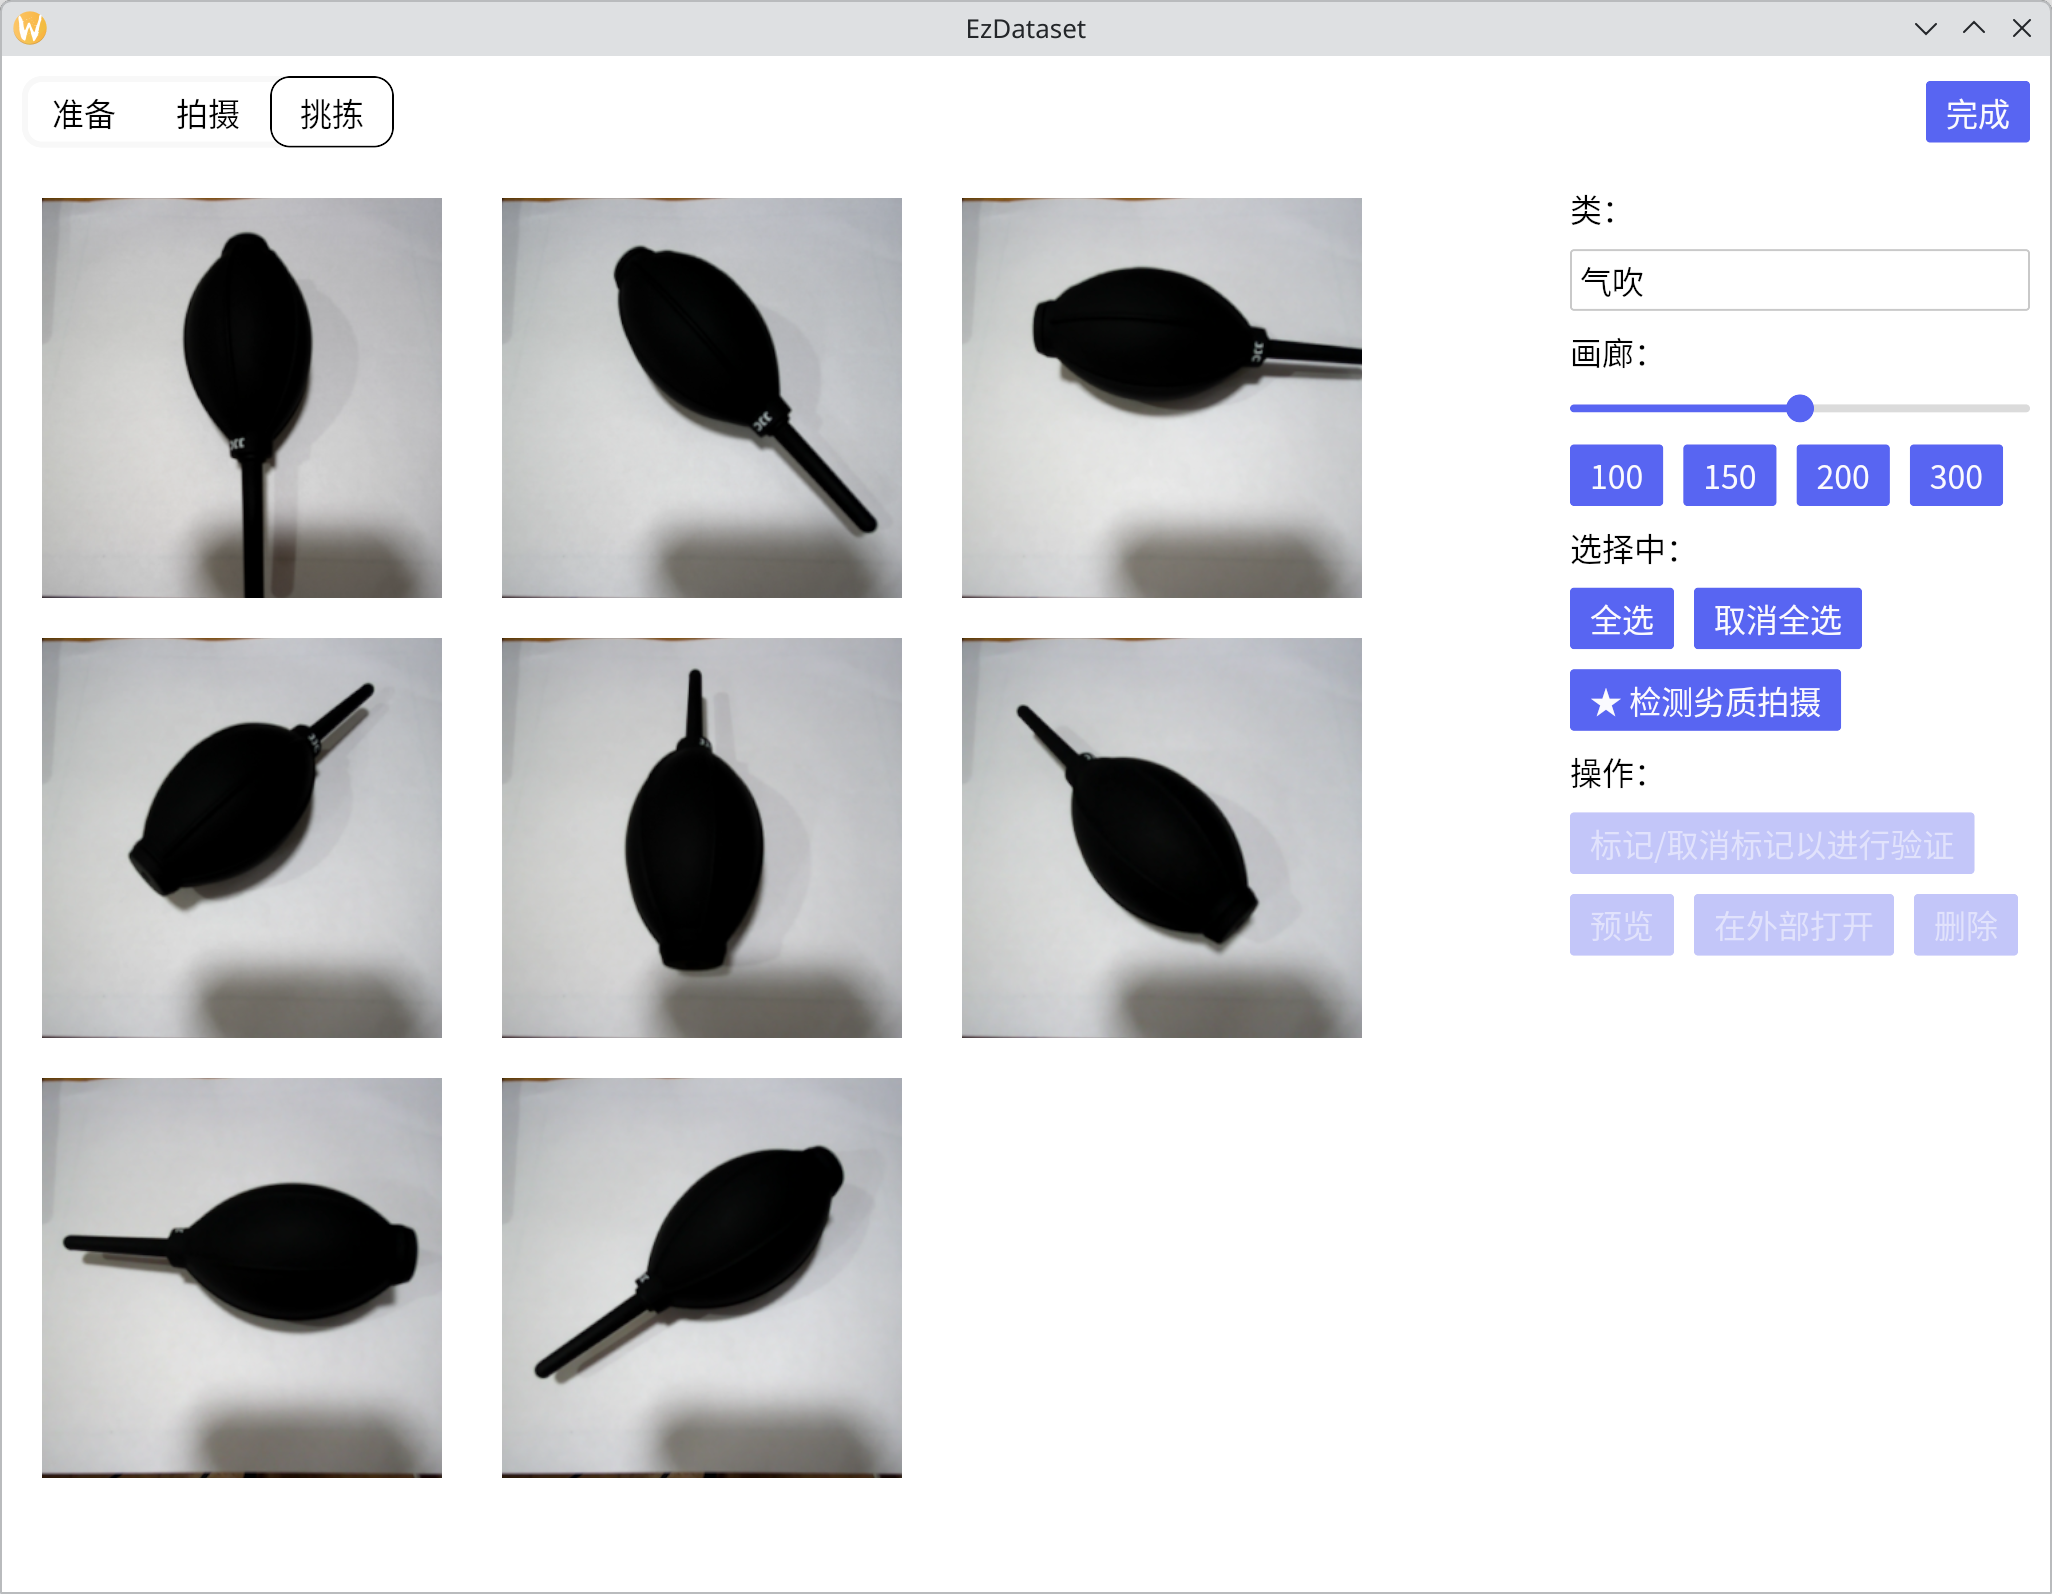
\includegraphics[width=0.33\textwidth]{./exp/ed-view.png}}
	\caption{EasyDataset运行效果:数据集编辑}
	\label{fig:ed-edit}
\end{figure}

创建数据集分为“准备”、“拍摄”和“挑拣”三步。如图 \ref{fig:ed-edit} 所示在准备界面(左),用户可以通过在两个输入框中输入类名和对应的商品编号来添加数据类别;在拍摄界面(中),用户利用单次拍摄或者连拍功能,并且以不同的方式在镜头前呈现商品,以此来拍摄高质量、符合推理环境的照片;在挑拣界面(右),用户可以对拍摄到的照片进行筛选,移除存在问题的照片并将某些照片标记为验证用途,用于测试模型泛化性能。

\subsection{顾客端}

\subsubsection{ShopEyes Guest}

\begin{figure}[htbp]
    \subfloat{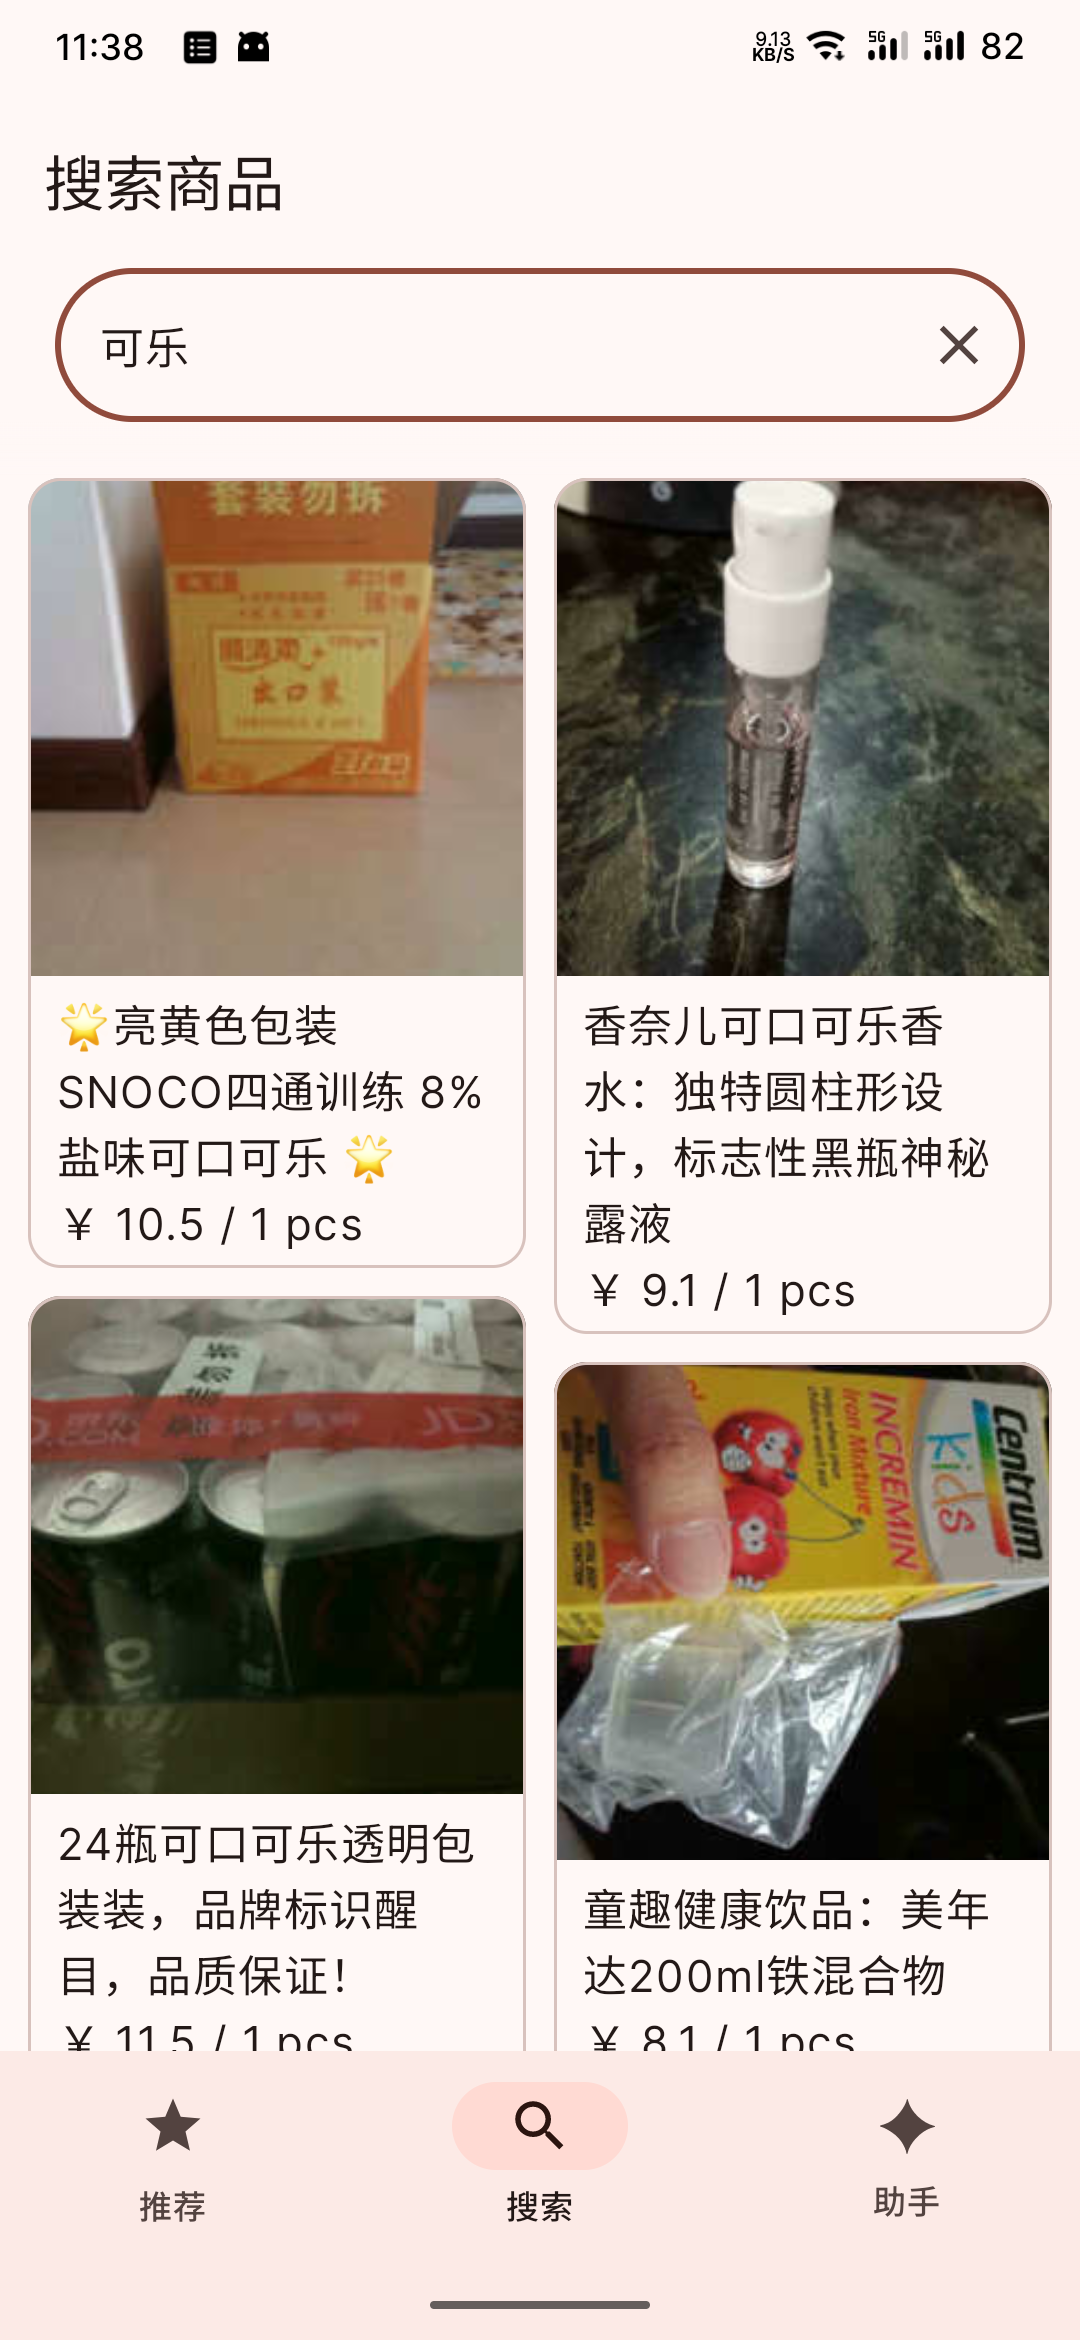
\includegraphics[width=0.3\textwidth]{./exp/seg-tx.png}}
    \hfill
    \subfloat{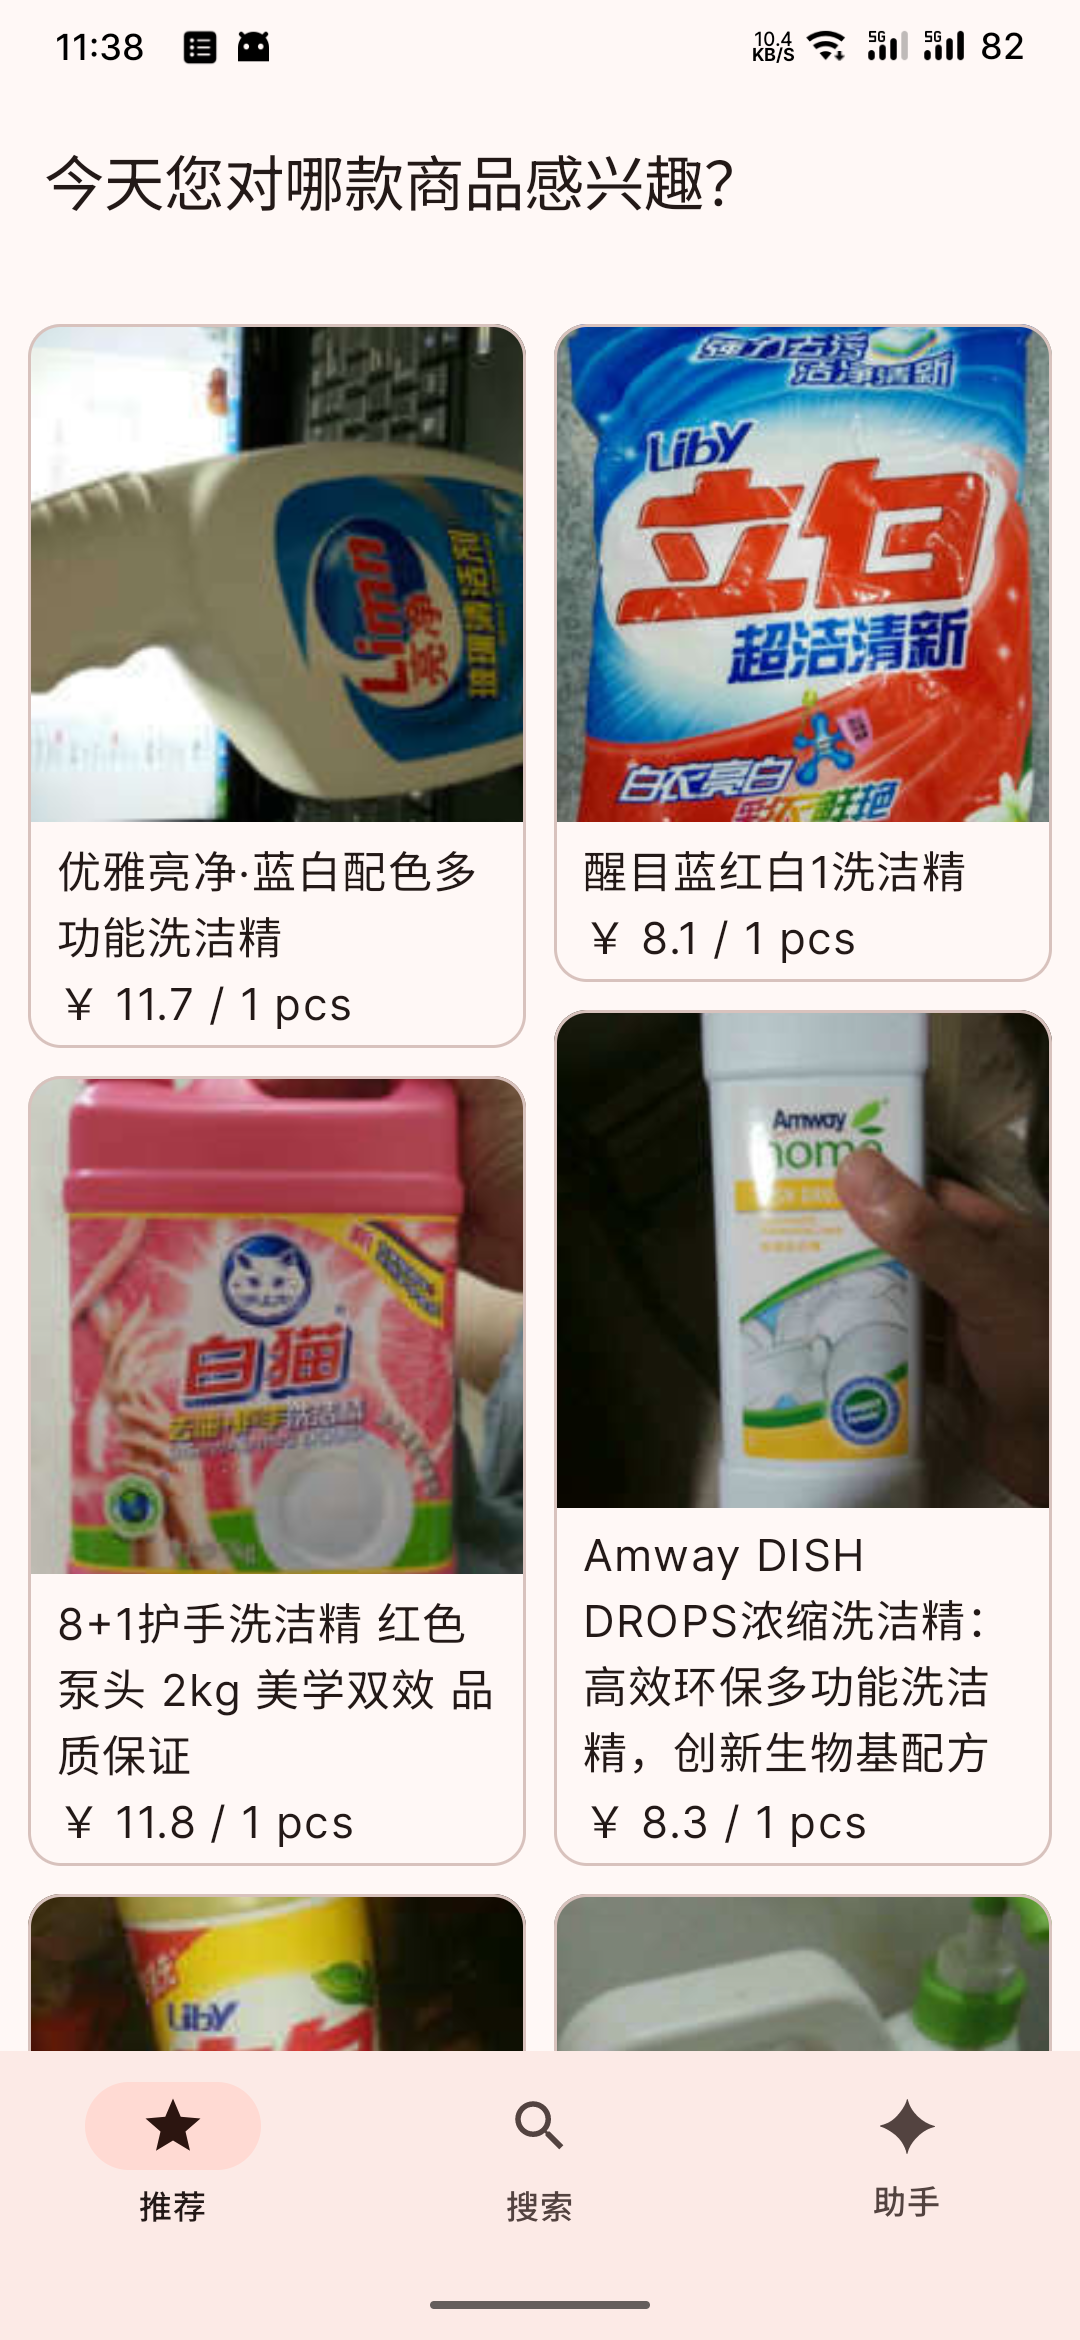
\includegraphics[width=0.3\textwidth]{./exp/seg-feat.png}}
    \hfill
    \subfloat{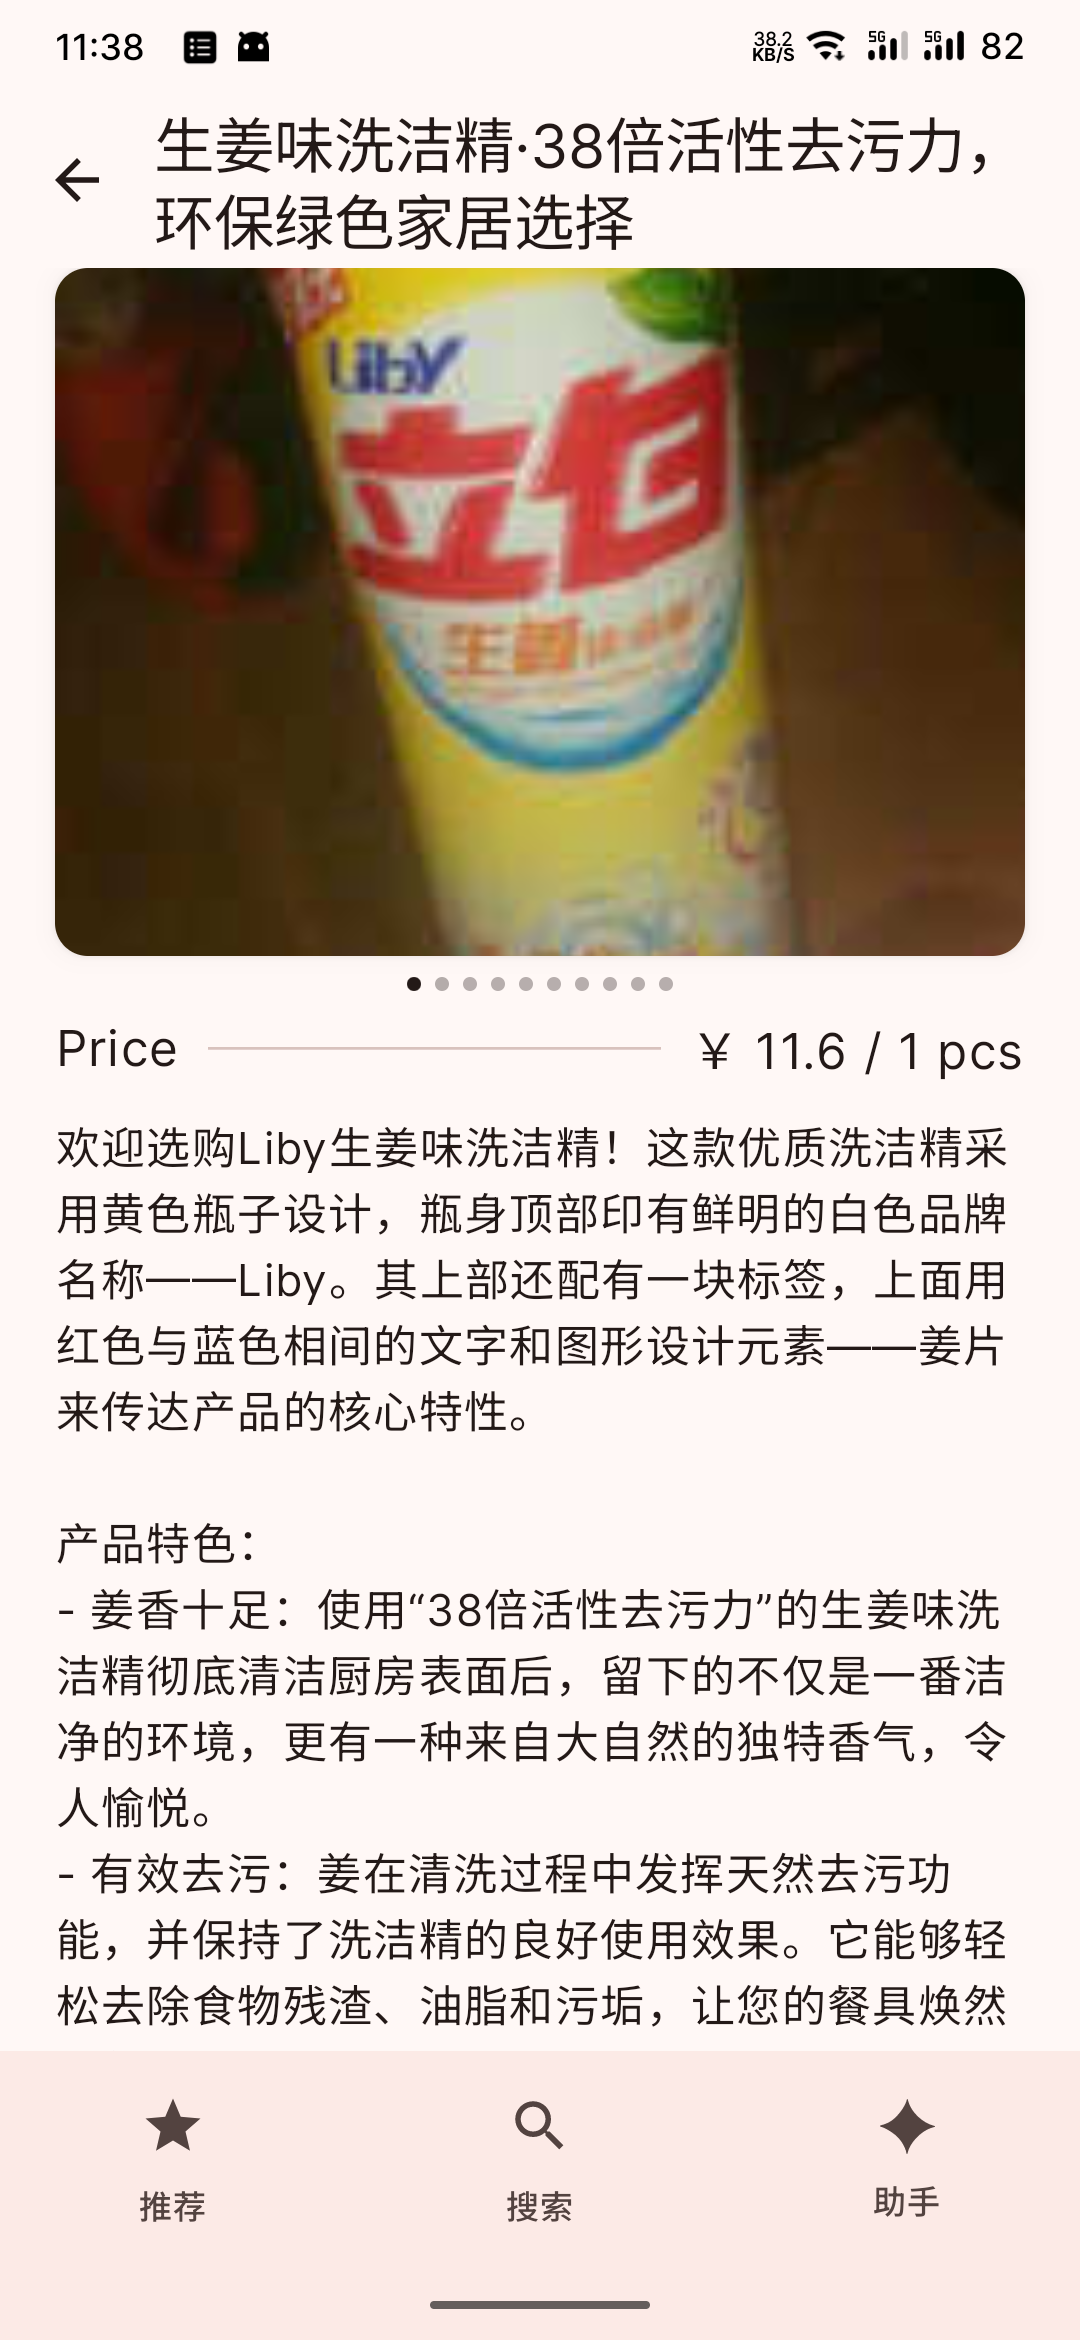
\includegraphics[width=0.3\textwidth]{./exp/seg-detail.png}}
	\caption{ShopEyes运行效果:基本功能}
	\label{fig:seg-generic}
\end{figure}

ShopEyes移动应用程序的顾客(Guest)端用于基于消费者商品信息查询和购买指引。如图所示,用户可以通过利用“推荐”界面(左)浏览由商家定义的推荐商品名录,也可以利用搜索功能(中;访问“探寻”搜索引擎)进行模糊搜索,对这些界面展示的商品信息,通过点击用户可以浏览对应商品的商品详情(右),其中包括详细介绍和价格等信息,也可以浏览商品的图片。

\begin{figure}[htbp]
    \centering
    \subfloat{
\includegraphics[width=0.25\textwidth]{./exp/seg-assist-1.png}}
    \hfill
    \subfloat{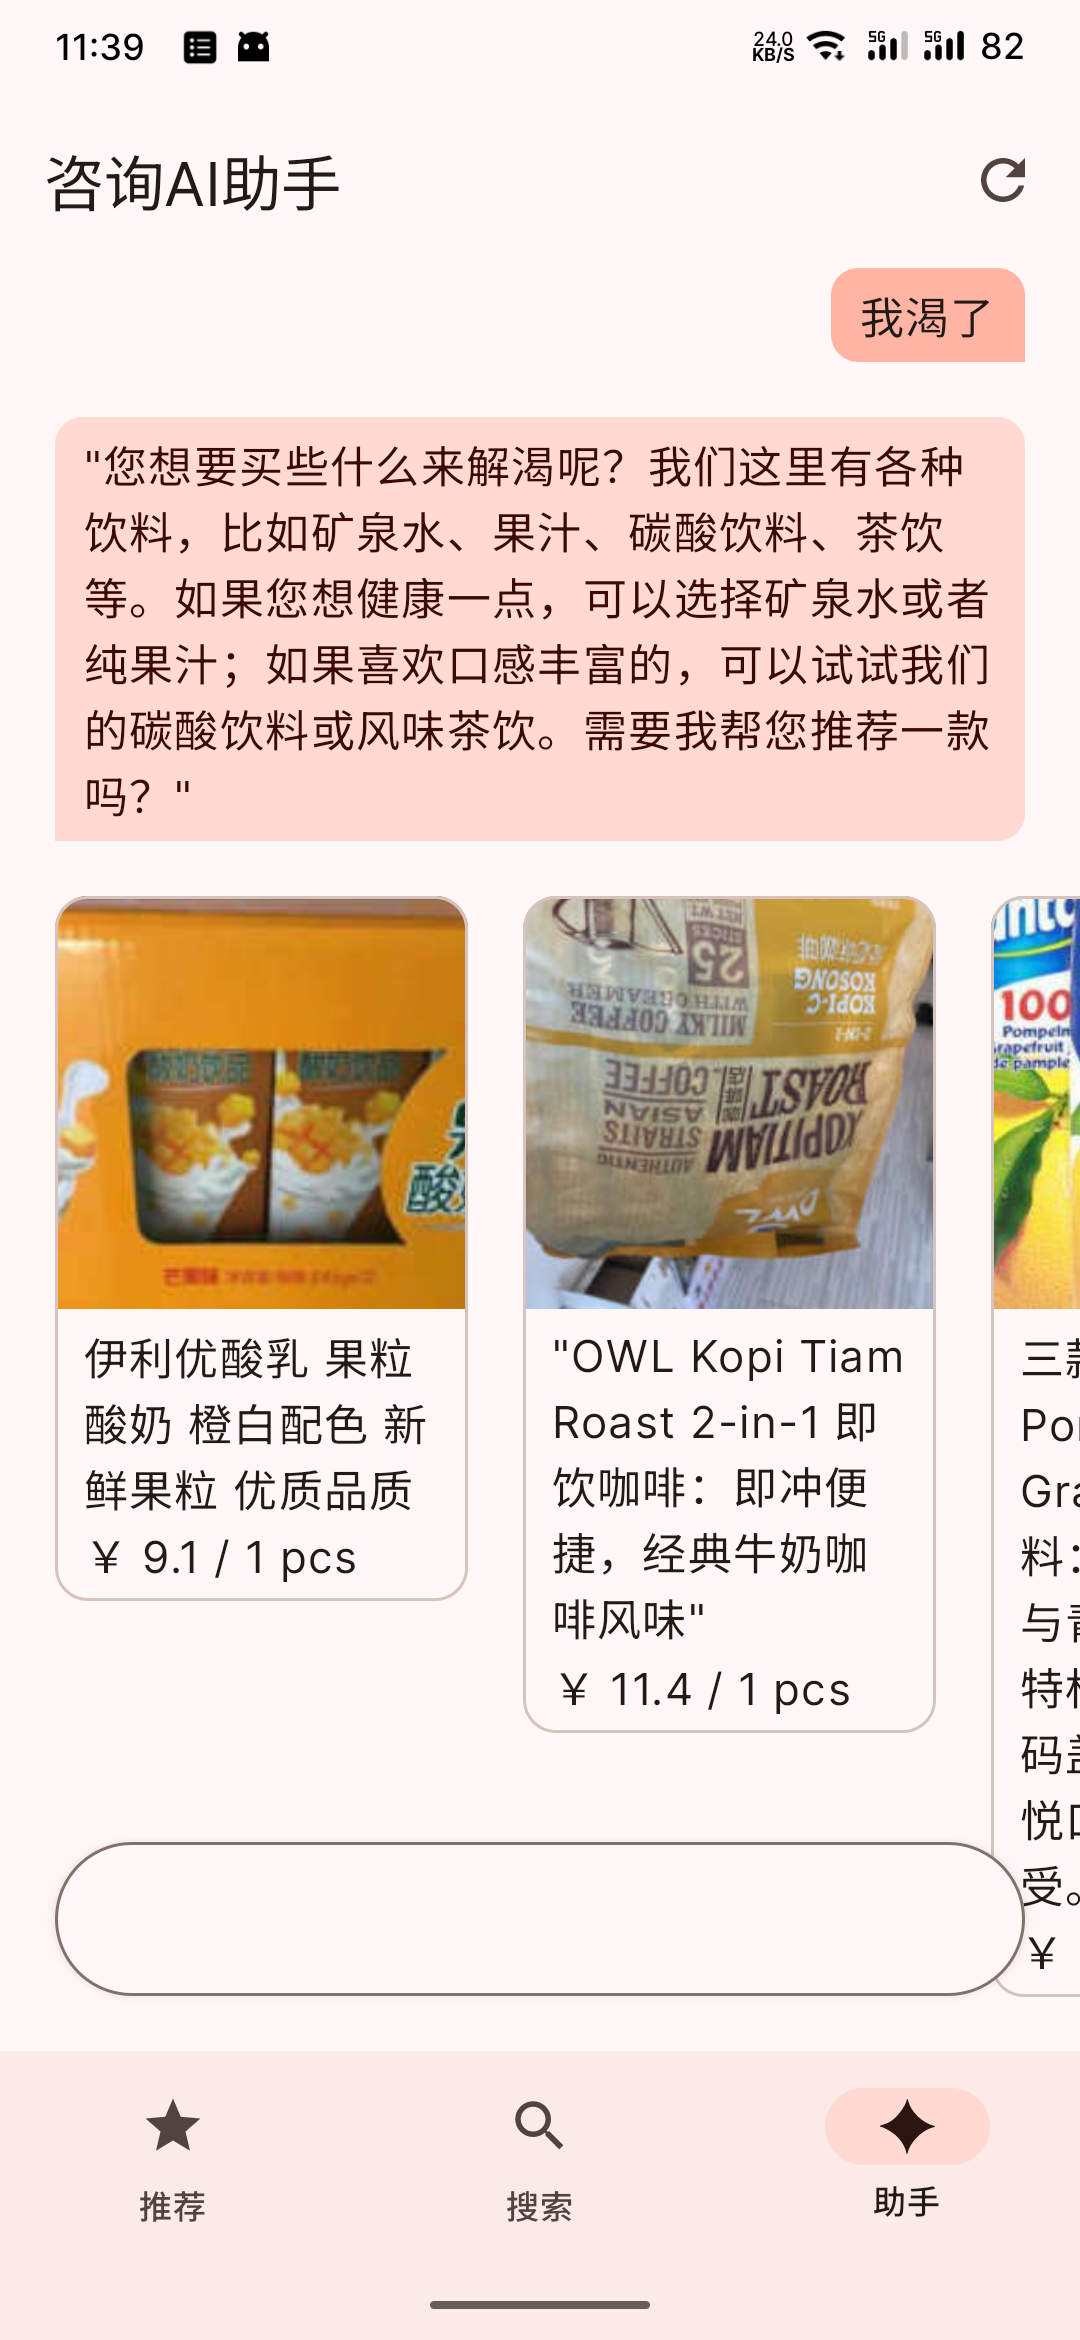
\includegraphics[width=0.25\textwidth]{./exp/seg-assist-2.png}}
	\caption{ShopEyes运行效果:AI导购}
	\label{fig:seg-assist}
\end{figure}

除此之外,用户还可以向AI询问购买建议。如图 \ref{fig:seg-assist} 所示,用户可以向AI描述自己的需要,并在下侧输入框中表达。点击发送按钮之后,输入框将展示用以提示用户思考过程政治进行的动画。操作完成之后,模型的输出和相应的商品推荐将被展示在对话中,用户也可以继续下一轮问题。

\subsubsection{EasyCheckout}

\begin{figure}[htbp]
    \centering
    \subfloat{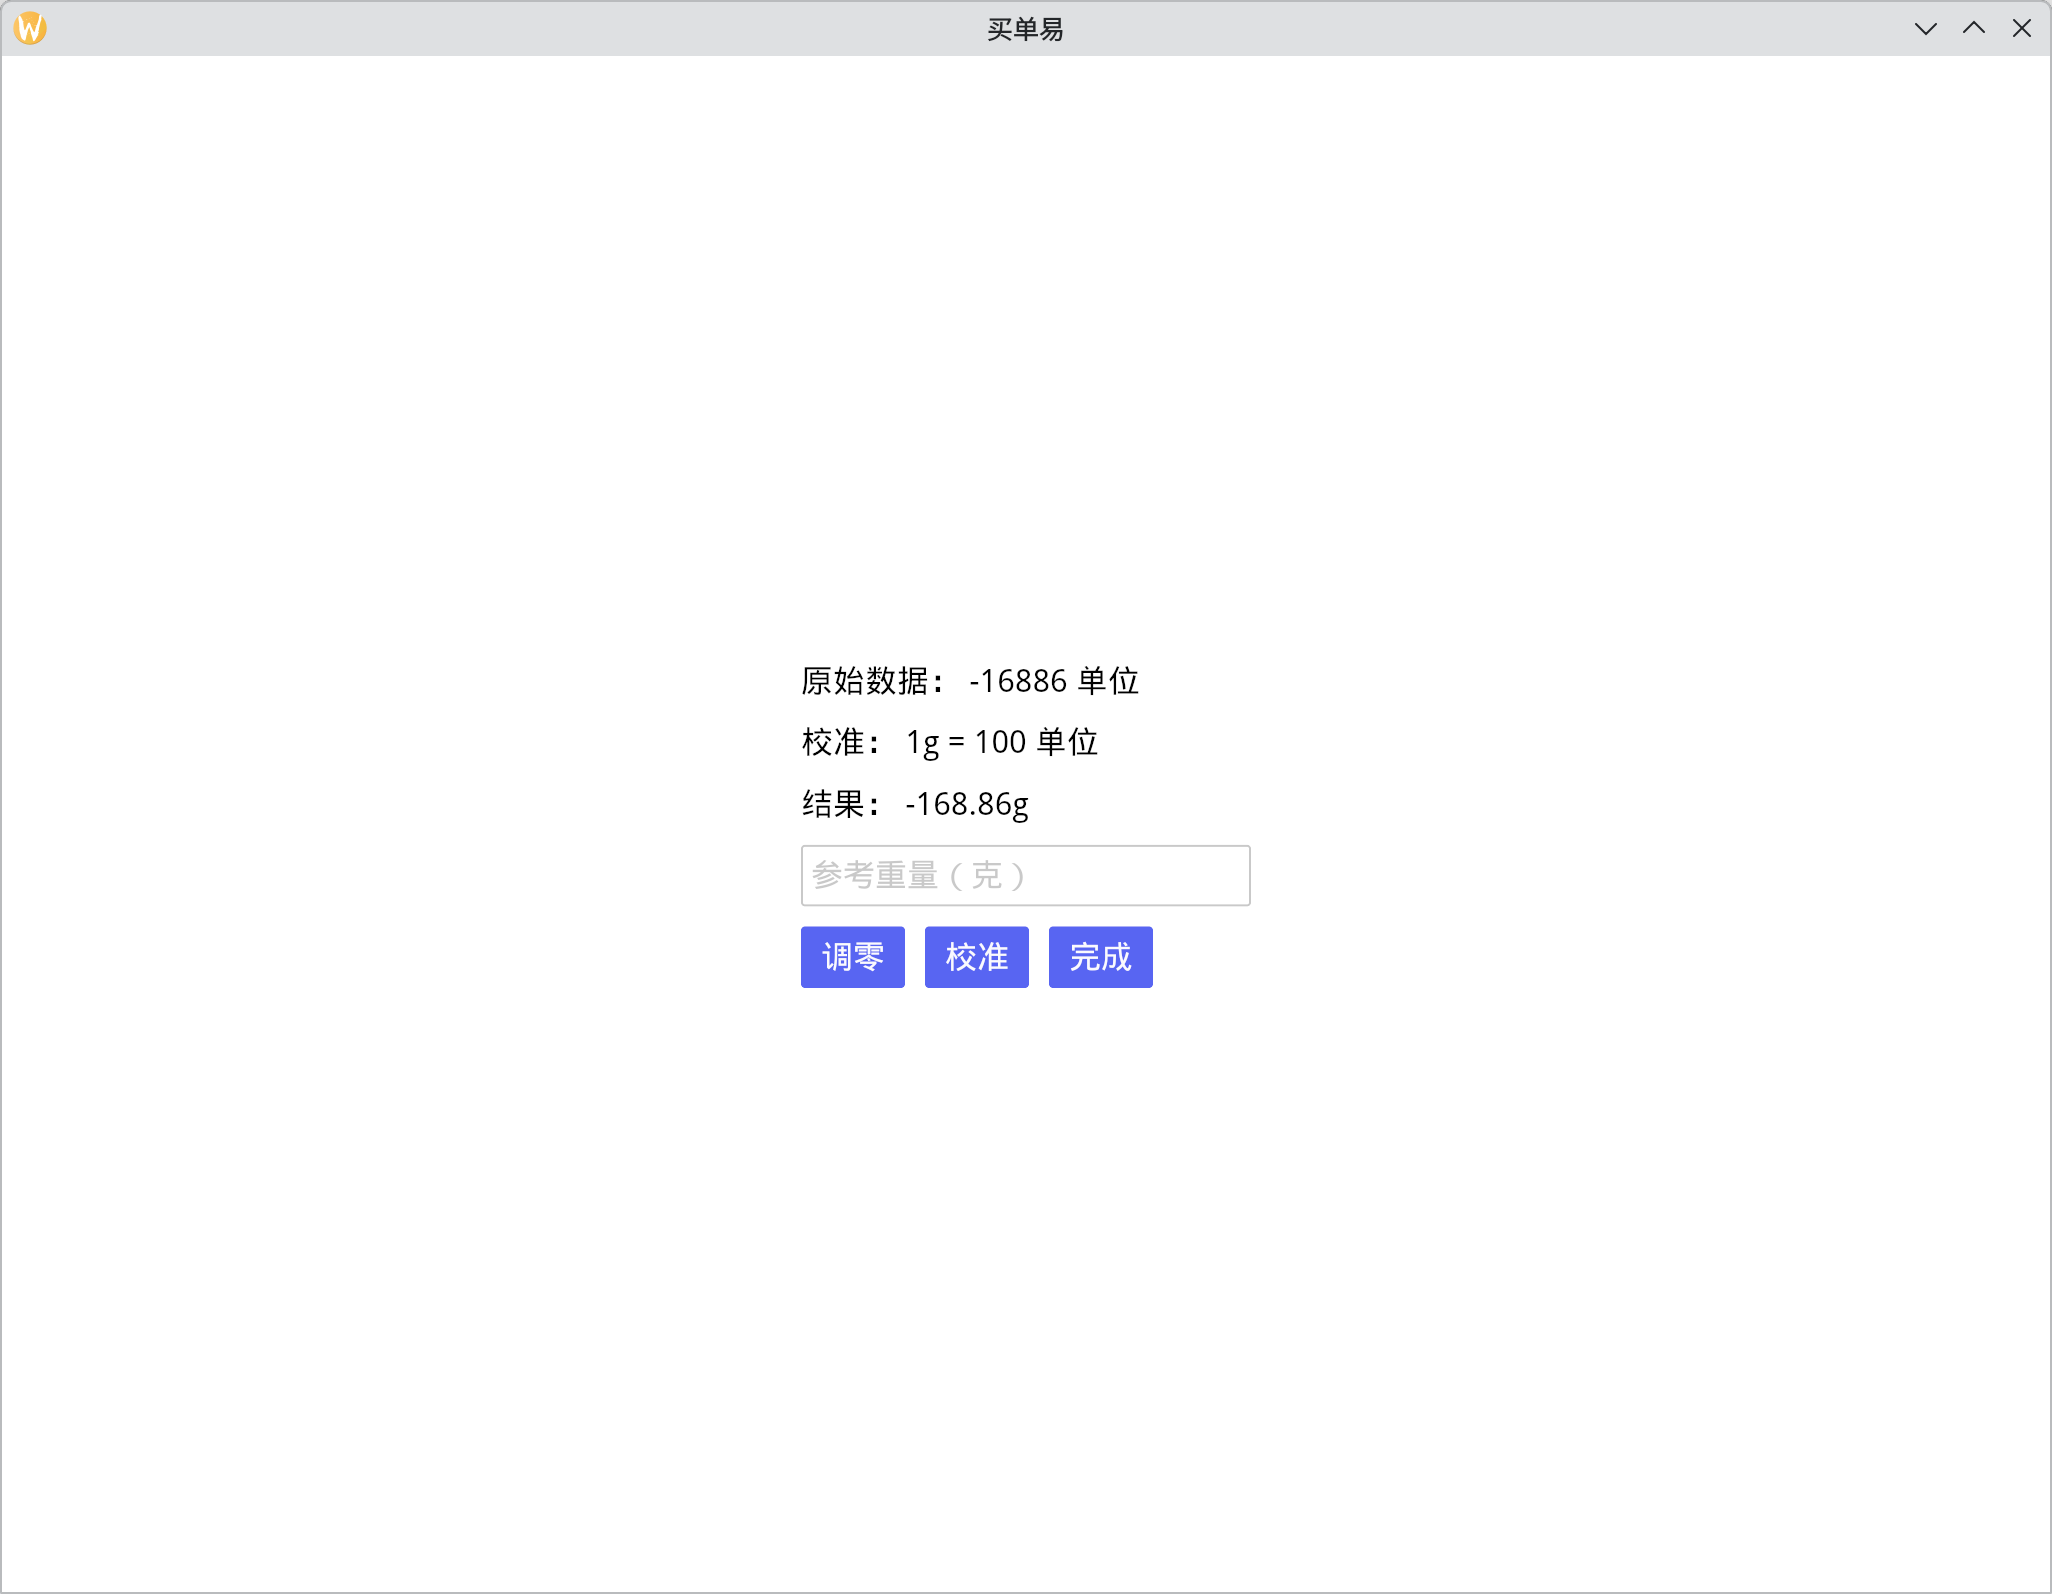
\includegraphics[width=0.4\textwidth]{./exp/ec-tare.png}}
    \hfill
    \subfloat{\includegraphics[width=0.4\textwidth]{./exp/ec-bc.png}}
    \vspace{1em}
    \subfloat{\includegraphics[width=0.4\textwidth]{./exp/ec-wr-1.png}}
    \hfill
    \subfloat{\includegraphics[width=0.4\textwidth]{./exp/ec-wr-2.png}}
	\caption{EasyCheckout运行效果}
	\label{fig:ec}
\end{figure}

应用程序EasyCheckout用于进行各种商品的结算。从图 \ref{fig:ec} 可见,营业者可以通过Ctrl-Shift-A快捷键唤出隐藏的调零和质量传感器校准界面(左上)进行必要的调整,而营业者或用户可以通过结算界面(右上)查看目前的商品或者通过条码扫描仪添加新的按件结算的商品。除此之外,通过点击“称重”按钮可以进入商品识别、称重整合的界面(左、右下),在此用户可以利用摄像头识别无标签的商品,并按重量添加到待结算商品列表。